% Options for packages loaded elsewhere
% Options for packages loaded elsewhere
\PassOptionsToPackage{unicode}{hyperref}
\PassOptionsToPackage{hyphens}{url}
\PassOptionsToPackage{dvipsnames,svgnames,x11names}{xcolor}
%
\documentclass[
  12pt,
]{report}
\usepackage{xcolor}
\usepackage[top = 3cm,bottom = 3cm,left = 3cm,right = 2.7cm]{geometry}
\usepackage{amsmath,amssymb}
\setcounter{secnumdepth}{5}
\usepackage{iftex}
\ifPDFTeX
  \usepackage[T1]{fontenc}
  \usepackage[utf8]{inputenc}
  \usepackage{textcomp} % provide euro and other symbols
\else % if luatex or xetex
  \usepackage{unicode-math} % this also loads fontspec
  \defaultfontfeatures{Scale=MatchLowercase}
  \defaultfontfeatures[\rmfamily]{Ligatures=TeX,Scale=1}
\fi
\usepackage{lmodern}
\ifPDFTeX\else
  % xetex/luatex font selection
  \setmainfont[]{Times New Roman}
  \setsansfont[]{Arial}
  \setmonofont[]{Courier New}
\fi
% Use upquote if available, for straight quotes in verbatim environments
\IfFileExists{upquote.sty}{\usepackage{upquote}}{}
\IfFileExists{microtype.sty}{% use microtype if available
  \usepackage[]{microtype}
  \UseMicrotypeSet[protrusion]{basicmath} % disable protrusion for tt fonts
}{}
\usepackage{setspace}
% Make \paragraph and \subparagraph free-standing
\makeatletter
\ifx\paragraph\undefined\else
  \let\oldparagraph\paragraph
  \renewcommand{\paragraph}{
    \@ifstar
      \xxxParagraphStar
      \xxxParagraphNoStar
  }
  \newcommand{\xxxParagraphStar}[1]{\oldparagraph*{#1}\mbox{}}
  \newcommand{\xxxParagraphNoStar}[1]{\oldparagraph{#1}\mbox{}}
\fi
\ifx\subparagraph\undefined\else
  \let\oldsubparagraph\subparagraph
  \renewcommand{\subparagraph}{
    \@ifstar
      \xxxSubParagraphStar
      \xxxSubParagraphNoStar
  }
  \newcommand{\xxxSubParagraphStar}[1]{\oldsubparagraph*{#1}\mbox{}}
  \newcommand{\xxxSubParagraphNoStar}[1]{\oldsubparagraph{#1}\mbox{}}
\fi
\makeatother


\usepackage{longtable,booktabs,array}
\usepackage{calc} % for calculating minipage widths
% Correct order of tables after \paragraph or \subparagraph
\usepackage{etoolbox}
\makeatletter
\patchcmd\longtable{\par}{\if@noskipsec\mbox{}\fi\par}{}{}
\makeatother
% Allow footnotes in longtable head/foot
\IfFileExists{footnotehyper.sty}{\usepackage{footnotehyper}}{\usepackage{footnote}}
\makesavenoteenv{longtable}
\usepackage{graphicx}
\makeatletter
\newsavebox\pandoc@box
\newcommand*\pandocbounded[1]{% scales image to fit in text height/width
  \sbox\pandoc@box{#1}%
  \Gscale@div\@tempa{\textheight}{\dimexpr\ht\pandoc@box+\dp\pandoc@box\relax}%
  \Gscale@div\@tempb{\linewidth}{\wd\pandoc@box}%
  \ifdim\@tempb\p@<\@tempa\p@\let\@tempa\@tempb\fi% select the smaller of both
  \ifdim\@tempa\p@<\p@\scalebox{\@tempa}{\usebox\pandoc@box}%
  \else\usebox{\pandoc@box}%
  \fi%
}
% Set default figure placement to htbp
\def\fps@figure{htbp}
\makeatother


% definitions for citeproc citations
\NewDocumentCommand\citeproctext{}{}
\NewDocumentCommand\citeproc{mm}{%
  \begingroup\def\citeproctext{#2}\cite{#1}\endgroup}
\makeatletter
 % allow citations to break across lines
 \let\@cite@ofmt\@firstofone
 % avoid brackets around text for \cite:
 \def\@biblabel#1{}
 \def\@cite#1#2{{#1\if@tempswa , #2\fi}}
\makeatother
\newlength{\cslhangindent}
\setlength{\cslhangindent}{1.5em}
\newlength{\csllabelwidth}
\setlength{\csllabelwidth}{3em}
\newenvironment{CSLReferences}[2] % #1 hanging-indent, #2 entry-spacing
 {\begin{list}{}{%
  \setlength{\itemindent}{0pt}
  \setlength{\leftmargin}{0pt}
  \setlength{\parsep}{0pt}
  % turn on hanging indent if param 1 is 1
  \ifodd #1
   \setlength{\leftmargin}{\cslhangindent}
   \setlength{\itemindent}{-1\cslhangindent}
  \fi
  % set entry spacing
  \setlength{\itemsep}{#2\baselineskip}}}
 {\end{list}}
\usepackage{calc}
\newcommand{\CSLBlock}[1]{\hfill\break\parbox[t]{\linewidth}{\strut\ignorespaces#1\strut}}
\newcommand{\CSLLeftMargin}[1]{\parbox[t]{\csllabelwidth}{\strut#1\strut}}
\newcommand{\CSLRightInline}[1]{\parbox[t]{\linewidth - \csllabelwidth}{\strut#1\strut}}
\newcommand{\CSLIndent}[1]{\hspace{\cslhangindent}#1}



\setlength{\emergencystretch}{3em} % prevent overfull lines

\providecommand{\tightlist}{%
  \setlength{\itemsep}{0pt}\setlength{\parskip}{0pt}}



 


\usepackage{booktabs}
\usepackage{caption}
\usepackage{longtable}
\usepackage{colortbl}
\usepackage{array}
\usepackage{anyfontsize}
\usepackage{multirow}
\usepackage{sectsty}
\chapterfont{\centering}
\usepackage{lscape}
\newcommand{\blandscape}{\begin{landscape}}
\newcommand{\elandscape}{\end{landscape}}
\makeatletter
\@ifpackageloaded{caption}{}{\usepackage{caption}}
\AtBeginDocument{%
\ifdefined\contentsname
  \renewcommand*\contentsname{Table of contents}
\else
  \newcommand\contentsname{Table of contents}
\fi
\ifdefined\listfigurename
  \renewcommand*\listfigurename{Figures}
\else
  \newcommand\listfigurename{Figures}
\fi
\ifdefined\listtablename
  \renewcommand*\listtablename{Tables}
\else
  \newcommand\listtablename{Tables}
\fi
\ifdefined\figurename
  \renewcommand*\figurename{Figure}
\else
  \newcommand\figurename{Figure}
\fi
\ifdefined\tablename
  \renewcommand*\tablename{Table}
\else
  \newcommand\tablename{Table}
\fi
}
\@ifpackageloaded{float}{}{\usepackage{float}}
\floatstyle{ruled}
\@ifundefined{c@chapter}{\newfloat{codelisting}{h}{lop}}{\newfloat{codelisting}{h}{lop}[chapter]}
\floatname{codelisting}{Listing}
\newcommand*\listoflistings{\listof{codelisting}{List of Listings}}
\makeatother
\makeatletter
\makeatother
\makeatletter
\@ifpackageloaded{caption}{}{\usepackage{caption}}
\@ifpackageloaded{subcaption}{}{\usepackage{subcaption}}
\makeatother
\usepackage{bookmark}
\IfFileExists{xurl.sty}{\usepackage{xurl}}{} % add URL line breaks if available
\urlstyle{same}
\hypersetup{
  colorlinks=true,
  linkcolor={blue},
  filecolor={Maroon},
  citecolor={Blue},
  urlcolor={blue},
  pdfcreator={LaTeX via pandoc}}


\author{}
\date{}
\begin{document}

\begin{titlepage}
  \begin{center}
    \vspace*{2cm}
    
    \Huge{\textbf{Leadership Transitions and Survival: Coups, Autocoups, and Power Dynamics}}
    
    \vspace{1.5cm}
    
    \Large{Zhu Qi}
    
    \vspace{2cm}
    
    \large{A thesis submitted for the degree of \\ Doctor of Philosophy in Political Science}
    
    \vspace{7cm}
    
    \large{Department of Government}
    \vspace{0.5cm}
    
    \large{University of Essex}
    
    \vspace{1.5cm}
    
    \large{September 2024}
    \vspace{2cm}
    
    
  \end{center}
\end{titlepage}

\renewcommand*\contentsname{Contents}
{
\hypersetup{linkcolor=}
\setcounter{tocdepth}{2}
\tableofcontents
}
\listoffigures
\listoftables

\setstretch{1.618}
\chapter*{Acknowledgements}\label{acknowledgements}
\addcontentsline{toc}{chapter}{Acknowledgements}

The completion of this thesis marks the culmination of a challenging yet
rewarding journey. I am deeply grateful to the numerous individuals who
have supported and encouraged me throughout this endeavour.

I would like to express my sincerest appreciation to my supervisor,
Professor Kristian Skrede Gleditsch, whose guidance, expertise, and
unwavering support have been instrumental in shaping my research. His
constructive feedback and encouragement have been invaluable, and I am
profoundly grateful for his mentorship.

I am also grateful to Professor Han Dorussen, the chair of my board
panel, for his continuous support and thoughtful input. His insightful
comments and suggestions have significantly enhanced the quality and
depth of my research.

I would like to acknowledge the important contributions of my initial
co-supervisors, Dr.~Saurabh Pant and Professor David Siroky, who laid a
strong foundation for this work during the early stages of my research.
Although they are no longer at the University of Essex, their
instruction and guidance were instrumental in shaping the direction of
this project.

I have been fortunate to receive feedback and guidance from several
esteemed scholars in the field, including Dr.~Brian J Phillips,
Dr.~Prabin Khadka, and Dr. Winnie Xia. Their expertise and insights have
enriched this research, and I am grateful for their contributions.

I would also like to express my sincere gratitude to my examiners,
Professor Tobias Böhmelt and Professor Jonathan Powell. Their insightful
questions, constructive critiques, and engaging discussion during the
viva examination (oral defense) were invaluable in challenging my
thinking and highlighting areas for further refinement. Their expertise
has undoubtedly strengthened the final version of this thesis.

On a personal note, I would like to express my deepest gratitude to my
family, who have been a constant source of support and inspiration
throughout this journey. To my beloved wife, Ji Zhi, your patience,
love, and encouragement have been immeasurable. To my dear children,
Siyan and Sisheng, your joy and curiosity have motivated me to persevere
and strive for excellence.

I am also deeply grateful to my father for his enduring support and
belief in my abilities. To the cherished memory of my late mother, your
love, guidance, and values continue to shape my path and inspire my
endeavours. And to my three brothers, whose support enabled me to pursue
my PhD without worries, I am forever grateful.

I take full responsibility for any errors or shortcomings in this work,
despite the invaluable contributions of many individuals.

\chapter*{Abstract}\label{abstract}
\addcontentsline{toc}{chapter}{Abstract}

This thesis addresses a significant gap in the literature on irregular
leadership transitions by systematically integrating autocoups---cases
where incumbent leaders extend their constitutionally mandated terms
through extra-constitutional means. It refines the conceptual definition
of autocoups, resolving existing ambiguities to align them more closely
with conventional coup frameworks. Based on this refined definition, the
thesis presents a novel global dataset of autocoup events from 1945 to
2023, encompassing 83 documented cases, of which 64 were successful.

Using this dataset, the study conducts a large-N analysis to identify
the structural determinants of autocoups. The findings reveal that
regimes with concentrated executive power, such as presidential
democracies and personalist regimes, are significantly more prone to
employing autocoups as a strategy for power retention compared to other
regime types. This pattern contrasts with traditional coups, which have
historically been more prevalent in military regimes.

The analysis subsequently examines leadership survival, utilising
survival analysis techniques to evaluate the political longevity of
leaders who assumed office through regular means, traditional coups, or
autocoups. Contrary to the hypothesis that the mode of power acquisition
significantly influences leadership survival---particularly the
expectation that autocoup leaders would enjoy longer tenures than those
installed through traditional coups---the results suggest that, when
excluding very short-lived tenures (i.e., less than 180 days), the mode
of accession does not exert a statistically significant effect on
leadership duration; instead, regime type emerges as the primary
determinant: leaders in military and personalist regimes exhibit
significantly higher hazard ratios for removal compared to the reference
category of dominant-party regimes, consistent with trends observed
following traditional coups.

The thesis further explores the broader institutional consequences of
irregular power transitions, focusing on their impact on
democratisation. Using Polity V scores as a proxy for democratic quality
and applying a country-fixed effects model, the analysis finds that
autocoups are associated with a sustained decline in democratic
indicators, both immediately after the event and over a two-year period;
in contrast, traditional coups exhibit a ``U-shaped'' effect: although
Polity V scores decline sharply in the immediate aftermath, they
typically recover to pre-coup levels within two years. These findings
highlight the divergent political trajectories triggered by coups and
autocoups, underscoring the need for increased scholarly and policy
attention to the persistently detrimental impact of autocoups on
democratic governance.

Collectively, these findings illuminate the distinct characteristics,
causes, and impacts of coups and autocoups. The research makes several
substantive contributions: it clarifies the conceptual boundaries of
autocoups, provides a new empirical foundation for their systematic
study, and offers robust comparative insights into how different modes
of irregular power transition affect leadership survival and
institutional development. These findings have significant implications
for academic scholarship and policy-making, particularly in the context
of global democratic backsliding and the resilience of political
institutions.

\emph{\textbf{Keywords:} Coups, Autocoups, Leadership transitions,
Leadership survival, Democratic resilience}

\chapter{Introduction}\label{introduction}

Why are some political leaders removed from office prematurely, while
others successfully extend their tenure beyond constitutionally mandated
limits? Moreover, how does the mode of their survival or removal
influence political stability and democratic institutions? This thesis
addresses these critical questions by analysing the structural and
strategic foundations of irregular leadership transitions.

\section{Rationale}\label{rationale}

The stability and resilience of political systems hinge on the orderly
transfer of power. Leadership transitions that occur within established
institutional frameworks reinforce political legitimacy and enhance
regime durability. Conversely, the breakdown of conventional mechanisms
for political succession often precipitates instability, violence, and
democratic backsliding. Among the most disruptive of these breakdowns
are irregular leadership transitions, which leave enduring institutional
legacies and fundamentally alter the political trajectories of regimes.
Understanding the causes and consequences of such events is central to
the study of political order and regime change.

The existing literature identifies diverse catalysts for irregular
leadership exits, including civil wars
(\citeproc{ref-kokkonen2019}{Kokkonen and Sundell 2019}), international
conflicts (\citeproc{ref-demesquita1995}{Mesquita and Siverson 1995}),
and ethnic divisions (\citeproc{ref-londregan1995}{Londregan, Bienen,
and Walle 1995}). Other factors include economic crises
(\citeproc{ref-miller2012}{M. K. Miller 2012};
\citeproc{ref-krishnarajan2019}{Krishnarajan 2019}) and natural
disasters (\citeproc{ref-quirozflores2012}{Quiroz Flores and Smith
2012}). Among these, coups d'état are particularly significant due to
their frequency and direct displacement of incumbent leaders. In
autocratic regimes, coups account for nearly one-third of all leadership
exits, surpassing regular transitions, which constitute just over
one-fifth (\citeproc{ref-frantz2016}{Frantz and Stein 2016}).
Furthermore, over \(63\%\) of non-constitutional removals in
dictatorships are attributable to coups
(\citeproc{ref-svolik2009}{Svolik 2009}).

Consequently, coups have garnered extensive scholarly attention, with a
substantial body of research exploring their causes, outcomes, and
long-term implications for democracy and development
(\citeproc{ref-thyne2019}{Thyne and Powell 2019}). The study of coup
determinants has flourished, with scholars proposing nearly one hundred
explanatory variables, yet a widely accepted baseline model remains
elusive (\citeproc{ref-gassebner2016}{Gassebner, Gutmann, and Voigt
2016}).

In contrast, autocoups---in which incumbent leaders extend their
constitutionally mandated terms through extra-constitutional means,
often by violating or circumventing provisions such as term limits or
succession rules---have received comparatively limited academic
attention. Although autocoups do not result in an immediate change of
leadership, they constitute a fundamental breach of institutional norms
governing political succession and disrupt the expected regular transfer
of power. Accordingly, they warrant classification as a critical, yet
underexamined, form of irregular leadership transition.

This thesis contends that autocoups warrant systematic analysis
alongside traditional coups within a unified analytical framework.
Despite differences in their execution, both coups and autocoups involve
extra-constitutional efforts to acquire or retain power and have
profound implications for leadership survival, regime stability, and
democratic integrity. A comparative analysis of these two forms of
irregular transition can elucidate shared drivers, divergent outcomes,
and broader lessons for democratic resilience.

The urgency of this inquiry is underscored by the significant risks
associated with irregular transitions. Both coups and autocoups can
trigger immediate crises---ranging from institutional paralysis to civil
unrest---and leave lasting institutional scars. More fundamentally, they
often dismantle constitutional checks and balances, undermine electoral
processes, and accelerate democratic decline or authoritarian
consolidation.

Historical cases vividly illustrate these dangers. Ghana's turbulent
period from 1979 to 1984 exemplifies the destabilising effects of
classic coups. Following Jerry Rawlings's 1979 coup, eight individuals,
including three former heads of state, were executed
(\citeproc{ref-pieterse1982}{Pieterse 1982}). Rawlings orchestrated
another coup in 1981 and subsequently suppressed three further coup
attempts (\citeproc{ref-haynes2022d}{Haynes 2022}). By contrast, the
1992 autocoup in Peru, led by President Alberto Fujimori, demonstrates
how an incumbent can dismantle democratic institutions without a change
in leadership. Fujimori dissolved Congress, suspended the constitution,
and ruled by decree (\citeproc{ref-mauceri1995}{Mauceri 1995};
\citeproc{ref-cameron1998}{Maxwell A. Cameron 1998b}).

These patterns are increasingly pertinent in the contemporary global
political landscape. According to Freedom House's Freedom in the World
2024 report, global political rights and civil liberties declined for
the eighteenth consecutive year in 2023, with setbacks recorded in 52
countries and improvements in only 21
(\citeproc{ref-freedomhouse2024freedom}{Freedom House 2024}). The
persistence of democratic erosion underscores the pressing need to
understand the mechanisms that facilitate it, including both coups and
autocoups.

This thesis aims to advance the theoretical and empirical understanding
of irregular leadership transitions. It offers insights with significant
implications for scholarly research and policy formulation, particularly
in fragile or democratising regimes.

\section{Research objectives and
contributions}\label{research-objectives-and-contributions}

In response to the significant challenges posed by irregular leadership
transitions, this study undertakes a comprehensive comparative analysis
structured around four core research objectives. Firstly, it aims to
refine the conceptual definition of autocoups and develop a novel
dataset suitable for large-N empirical analysis. Secondly, it seeks to
identify the structural and institutional determinants of autocoups
through systematic quantitative investigation. Thirdly, it compares the
survival prospects of leaders who assume power through traditional coups
with those who extend their tenure via autocoups. Finally, it evaluates
the divergent impacts of coups and autocoups on democratisation
trajectories and the resilience of political institutions.

By examining both coups and autocoups from 1945 to 2023, this thesis
addresses a critical gap in political science by developing and applying
a unified analytical framework that treats these events as distinct yet
interrelated forms of extra-constitutional power transition. Through
this approach, the study makes four principal contributions to the
literature on leadership dynamics, regime stability, and institutional
development.

\textbf{Conceptual clarification and empirical foundation for
autocoups:} This thesis enhances conceptual clarity by situating
autocoups within the broader typology of irregular power transitions. It
provides a refined definition of autocoups, focusing on the executive's
unilateral extension of tenure through extra-constitutional means, and
clearly distinguishes them from executive aggrandisement and traditional
military coups. Building on this conceptual framework, the study
introduces an original dataset of autocoup events from 1945 to 2023,
documenting 83 incidents, of which 64 were successful. This dataset
addresses a long-standing empirical gap and establishes a robust
foundation for systematic comparative analysis, enabling future research
into a previously understudied form of institutional disruption.

\textbf{First empirical analysis of autocoup determinants}: Utilising
the newly compiled dataset, the thesis conducts the first empirical
examination of the structural and institutional conditions conducive to
autocoups. The analysis reveals that leaders in power-concentrated
systems---particularly presidential democracies and personalist
regimes---are significantly more likely to extend their tenure through
autocoups compared to those in other regime types. These findings
contribute to the literature on the interplay between regime
characteristics and irregular power retention, highlighting the pivotal
role of institutional structures in shaping leaders' strategic decisions
to circumvent term limits.

\textbf{Comparative analysis of leadership longevity}: The research
advances the study of leadership survival by comparing the tenure
durations of leaders who attain power through regular means, traditional
coups, or autocoups. Employing survival analysis, the study finds that,
contrary to expectations, the mode of power acquisition does not
significantly predict leadership longevity. However, it reaffirms the
decisive influence of regime type on leader survival, regardless of the
mode of accession or retention. The survival models indicate that
leaders in military and personalist regimes face higher hazard ratios
for removal compared to those in dominant-party regimes. These results
underscore the critical influence of regime structure on leadership
durability and elite turnover.

\textbf{Comparative democratic implications of coups and autocoups}: The
thesis further investigates the differential impacts of coups and
autocoups on democratic development. Using country-fixed effects
regression models and Polity V scores as an indicator of democratic
quality, the analysis demonstrates that autocoups are associated with a
gradual and sustained decline in Polity V scores, both immediately
following the event and over a two-year period. In contrast, coups
result in a ``U-shaped'' institutional outcome: while they precipitate
immediate declines in Polity V scores, these typically recover to
pre-event levels within two years. This disaggregated analysis
illuminates the distinct trajectories and institutional consequences of
different forms of irregular power transitions.

Collectively, these contributions provide a robust theoretical and
empirical foundation for understanding the dynamics of irregular
leadership transitions, offering significant insights for both academic
scholarship and policy formulation in the context of democratic
resilience and institutional stability.

\section{Policy implications}\label{policy-implications}

Although scholarly debate continues regarding the potential for coups to
inadvertently foster democratisation under specific circumstances
(\citeproc{ref-thyne2014}{C. Thyne and Powell 2014};
\citeproc{ref-derpanopoulos2016}{Derpanopoulos et al. 2016};
\citeproc{ref-miller2016}{M. K. Miller 2016}), a robust policy consensus
holds that coups represent inherently illegitimate mechanisms of
political change. As violent disruptions of constitutional order, they
typically inflict immediate institutional damage, precipitate
instability, and result in unpredictable political trajectories.
Consequently, both international and domestic policy responses have
prioritised prevention, most notably through `coup-proofing' strategies
aimed at insulating regimes from military intervention or elite
defection (\citeproc{ref-quinlivan1999}{Quinlivan 1999};
\citeproc{ref-pilster2012}{Pilster and Böhmelt 2012};
\citeproc{ref-powell2012coups}{J. Powell 2012a};
\citeproc{ref-albrecht2014}{Albrecht 2014a};
\citeproc{ref-carey2015}{Carey, Colaresi, and Mitchell 2015};
\citeproc{ref-brown2015}{C. S. Brown, Fariss, and McMahon 2015};
\citeproc{ref-sudduth2017}{Sudduth 2017}). However, as this thesis
demonstrates, such approaches have well-documented limitations
(\citeproc{ref-albrecht2014a}{Albrecht 2014b};
\citeproc{ref-reiter2020}{Reiter 2020}), and deeper structural power
dynamics within regimes are often more critical in determining
vulnerability to both coups and autocoups.

The findings of this study yield several important policy implications,
particularly in the domains of institutional design, international
responses, and the monitoring of democratic backsliding. In terms of
institutional design, the research highlights the heightened
susceptibility of power-concentrated systems---such as presidential
democracies and personalist regimes---to autocoups. This underscores the
importance of reinforcing institutional checks and balances through
mechanisms such as independent judiciaries, robust legislative
oversight, and clearly defined constitutional term limits, all of which
serve to constrain executive overreach and mitigate the risk of
extra-constitutional power consolidation. With regard to international
responses, the persistent democratic erosion associated with
autocoups---evidenced by sustained declines in Polity V scores---calls
for proactive diplomatic and economic interventions. These may include
targeted sanctions, conditional aid, or other measures aimed at
deterring incumbent leaders from circumventing constitutional safeguards
in an effort to prolong their tenure. Moreover, the effective monitoring
of democratic backsliding requires more sophisticated frameworks capable
of detecting early warning signs of autocoups. These signs often
manifest in gradual and legally veiled efforts to undermine term-limit
provisions or manipulate electoral processes, in contrast to the more
abrupt and overt power seizures typical of traditional coups. These
policy implications, which call for tailored approaches to address the
distinct dynamics of coups and autocoups, will be examined further in
the concluding chapter.

\section{Limitations and future
research}\label{limitations-and-future-research}

Whilst this study proposes a novel analytical framework for
understanding coups and autocoups, their impact on leadership survival,
and their broader institutional consequences, several limitations
persist, pointing to significant opportunities for future research and
refinement.

A primary challenge lies in the conceptual ambiguity surrounding the
definition of autocoups, particularly in borderline cases where
incumbents extend their authority through legal or quasi-legal
mechanisms. Future research could explore the normative and analytical
trade-offs of including such cases within the autocoup category.
Comparative analyses of `unconstitutional' versus `extra-constitutional'
extensions of executive tenure may help determine whether these actions
represent variants of the same phenomenon or distinct processes.
President Manuel Zelaya's 2009 attempt to amend the Honduran
constitution to permit future re-election triggered a military coup that
removed him from office
(\citeproc{ref-muuxf1oz-portillo2019}{Muñoz-Portillo and Treminio
2019}). This case exemplifies the analytical complexity of identifying
autocoups and highlights the need for refined coding criteria and
greater interpretive clarity in future data collection efforts.

Given the long-term decline in traditional coups and the concurrent rise
of autocoups, increased scholarly focus on the latter is essential.
Although this study centres on tenure extension as the defining
characteristic of autocoups, broader forms of executive power
expansion---whether within or beyond formal constitutional
frameworks---warrant systematic investigation. The development of a
dedicated dataset on executive power expansion would be a critical step
towards capturing the full spectrum of such practices.

Furthermore, the decreasing frequency of overt and dramatic regime
transitions since the early 2000s, coupled with a reduction in clear
shifts between democracy and autocracy, highlights the need for more
sensitive analytical tools to detect incremental changes within regimes.
Future empirical research should prioritise the identification and
measurement of these subtler transformations to better understand their
implications for regime stability and democratic resilience.

These limitations and promising avenues for future inquiry will be
examined in greater detail in the concluding chapter.

\section{Overview of the thesis}\label{overview-of-the-thesis}

This thesis examines the intricate power dynamics underlying coups and
autocoups, focusing on their consequences for leadership survival and
the democratisation or authoritarian transformation of political
regimes. It develops a unified analytical framework to study these
phenomena as distinct yet interconnected forms of irregular power
transition. Each chapter contributes to this overarching inquiry by
providing conceptual clarifications, empirical innovations, and
comparative insights.

\subsection*{Chapter 2: Autocoups: Conceptual Clarification and Dataset
Introduction}\label{chapter-2-autocoups-conceptual-clarification-and-dataset-introduction}
\addcontentsline{toc}{subsection}{Chapter 2: Autocoups: Conceptual
Clarification and Dataset Introduction}

Despite the rising prevalence of autocoups, particularly in the
post-Cold War era, their systematic study remains underdeveloped. The
existing literature suffers from conceptual fragmentation, marked by a
proliferation of overlapping and inconsistently defined terms (e.g.,
`self-coup', `autogolpe', `executive aggrandisement')
(\citeproc{ref-marsteintredet2019}{Marsteintredet and Malamud 2019};
\citeproc{ref-baturo2022}{Baturo and Tolstrup 2022}). This conceptual
ambiguity hinders empirical analysis, as many datasets fail to
distinguish between tenure extension and other forms of executive power
consolidation---a critical distinction for this study. Consequently,
methodological progress has been limited, with most research relying on
qualitative case studies (\citeproc{ref-cameron1998}{Maxwell A. Cameron
1998b}; \citeproc{ref-antonio2021}{Antonio 2021};
\citeproc{ref-pion-berlin2022}{Pion-Berlin, Bruneau, and Goetze 2022})
rather than quantitative analyses.

This chapter addresses these shortcomings by proposing a precise and
theoretically grounded definition of the autocoup, centred on attempts
by incumbents to extend their constitutionally mandated terms of office
through extra-constitutional means. By focusing on tenure extension, the
definition excludes broader forms of executive aggrandisement that occur
within existing constitutional timeframes, aligning autocoups
conceptually with traditional coups, both of which disrupt
constitutionally prescribed leadership succession. Building on this
definition, the chapter introduces a significant empirical contribution:
an original global dataset of autocoups from 1945 to 2023, documenting
83 distinct events, of which 64 were successful. This dataset enables
systematic quantitative analysis and opens new avenues for comparative
research on irregular power retention.

\subsection*{Chapter 3: Power Dynamics and Autocoup
Attempts}\label{chapter-3-power-dynamics-and-autocoup-attempts}
\addcontentsline{toc}{subsection}{Chapter 3: Power Dynamics and Autocoup
Attempts}

Due to long-standing conceptual and empirical constraints, prior
discussion of autocoups have predominantly relied on case-based
approaches (\citeproc{ref-baturo2019politics}{Baturo and Elgie 2019};
\citeproc{ref-marsteintredet2019}{Marsteintredet and Malamud 2019};
\citeproc{ref-baturo2022}{Baturo and Tolstrup 2022}). The dataset
introduced in Chapter 2 facilitates, for the first time, a broad
empirical study of the structural conditions underpinning autocoup
attempts.

Drawing on insights from the coup literature, this chapter examines a
range of potential predictors, including economic performance,
succession rules, military influence, protest activity, and media
freedom. While these variables have been explored in the context of
traditional coups, they often fail to account for persistent
cross-regime variation or the limited efficacy of `coup-proofing'
strategies (\citeproc{ref-albrecht2014a}{Albrecht 2014b};
\citeproc{ref-reiter2020}{Reiter 2020}). Moreover, many studies employ
overly simplistic regime typologies (e.g., democracy versus autocracy,
or civilian versus military), obscuring significant variation within
regime types (\citeproc{ref-hiroi2013}{Hiroi and Omori 2013};
\citeproc{ref-schiel2019}{Schiel 2019}).

This chapter argues that the risk of autocoups is fundamentally shaped
by the structural balance of power established at a regime's inception.
Specifically, the likelihood of an autocoup is determined by the
equilibrium between incumbents and potential institutional challengers
(\citeproc{ref-geddes2014}{Geddes, Wright, and Frantz 2014}). Using
regime typologies as proxies for internal power structures, the analysis
employs both a standard logit model and a bias-reduced logit model
(Firth's penalised maximum likelihood estimation). The results
demonstrate that presidential democracies and personalist regimes are
significantly more prone to autocoup attempts than dominant-party
regimes, when controlling for other variables. By contrast, leaders in
dominant-party and military regimes exhibit no significant difference in
their likelihood of attempting an autocoup. These findings highlight the
critical role of regime type in shaping elite incentives for irregular
tenure extension.

\subsection*{Chapter 4: Power Acquisition and Leadership
Survival}\label{chapter-4-power-acquisition-and-leadership-survival}
\addcontentsline{toc}{subsection}{Chapter 4: Power Acquisition and
Leadership Survival}

Although extensive research has examined the tenure survival of leaders
who assume power through coups (\citeproc{ref-gandhi2007}{Gandhi and
Przeworski 2007}; \citeproc{ref-sudduth2017}{Sudduth 2017};
\citeproc{ref-easton2018}{Easton and Siverson 2018}), the lack of
comparable data on autocoups has precluded systematic comparisons among
regular-entry leaders, coup-installed leaders, and autocoup leaders.
This chapter addresses this gap by conducting the first comparative
survival analysis of these three categories within a unified theoretical
framework.

It posits that coup-installed leaders typically face heightened
legitimacy deficits, political uncertainty, and institutional
instability, whereas autocoup leaders benefit from institutional
continuity while dismantling key constraints. These differing conditions
shape distinct pathways to political consolidation. Notably, the
time-dependent Cox model reveals no statistically significant difference
in survival risk among regular-entry, coup-installed, and autocoup
leaders once relevant covariates---particularly regime type---are
accounted for. Instead, regime characteristics exert a decisive
influence on leadership tenure: leaders in military and personalist
regimes face significantly higher risks of removal compared to those in
dominant-party regimes.

\subsection*{Chapter 5: Coups, autocoups, and
democracy}\label{chapter-5-coups-autocoups-and-democracy}
\addcontentsline{toc}{subsection}{Chapter 5: Coups, autocoups, and
democracy}

While the impact of coups on democratisation has been widely studied
(\citeproc{ref-clayton2000}{Clayton and Onwumechili 2000};
\citeproc{ref-powell2014a}{J. Powell 2014}; \citeproc{ref-thyne2020}{C.
Thyne and Hitch 2020}), the consequences of autocoups remain
underexplored due to the historical absence of relevant data. This
chapter addresses this gap through a quantitative analysis of how coups
and autocoups affect democratic institutions.

Whereas coups often result in leadership turnover or regime change,
autocoups typically involve incumbents dismantling institutional
constraints without altering the core ruling coalition. Consequently,
their effects are best assessed through continuous measures of
democratic quality, such as Polity V scores, rather than binary
regime-type transitions. The chapter argues that autocoups lead to
consistent declines in Polity V scores, while coups produce more complex
impacts. Empirical analysis using a country-fixed effects model confirms
that autocoups are associated with sustained reductions in Polity V
scores both immediately following the event and over a two-year period.
In contrast, coups cause an initial decline in Polity V scores but often
exhibit a ``U-shaped'' recovery within two years. These findings
underscore the uniquely insidious nature of autocoups, which frequently
proceed incrementally under a legalistic façade.

\subsection*{Chapter 6: Conclusion and future research
directions}\label{chapter-6-conclusion-and-future-research-directions}
\addcontentsline{toc}{subsection}{Chapter 6: Conclusion and future
research directions}

The concluding chapter synthesises the findings of the preceding
chapters, highlighting the structural, strategic, and institutional
dynamics that underpin irregular leadership transitions. It argues that
coups and autocoups are not merely disruptive events but strategic tools
employed by elites to recalibrate or entrench political authority. Their
institutional legacies diverge: while coups often destabilise regimes,
autocoups typically consolidate autocratic rule.

This chapter outlines the broader implications of these findings for
understanding the resilience of autocracy, the vulnerability of
democratic institutions, and the strategic calculus of political
leaders. It also proposes several directions for future research,
including further exploration of the nuances of executive power
expansion and the development of more sensitive measures to detect
incremental regime changes.

\chapter{Autocoups: Conceptual Clarification and Dataset
Introduction}\label{sec-chapter3}

\section*{Abstract}\label{abstract-1}
\addcontentsline{toc}{section}{Abstract}

This chapter proposes a refined conceptualisation of autocoups, defined
as instances where incumbent leaders extend their constitutionally
mandated tenure through extra-constitutional means, typically by
circumventing or breaching term limits. By critically reviewing and
synthesising overlapping terms---such as `self-coup', `autogolpe', and
`executive takeover'---the chapter delineates the conceptual boundaries
of the phenomenon, establishing tenure extension as its defining
feature. In distinguishing autocoups from broader and more ambiguous
forms of executive aggrandisement, it advances a more analytically
precise framework for examining irregular power extensions. Building on
this conceptual foundation, the chapter introduces an original global
dataset of autocoup events from 1945 to 2023, documenting 83 distinct
cases, of which 64 were successful. This empirical contribution
facilitates systematic, large-N analysis of an increasingly prevalent
mode of authoritarian consolidation.

\emph{\textbf{Keywords}: Autocoups, Coups, Irregular Power Transitions,
Leadership Tenure, Dataset}

\section{Introduction}\label{introduction-1}

The stability and resilience of political systems depend fundamentally
on the orderly transfer of power. When leadership succession occurs
within established constitutional frameworks, it bolsters the legitimacy
and durability of governing institutions. Conversely, the breakdown of
these norms often precipitates political violence, institutional
erosion, and prolonged instability

Although many leadership transitions occur smoothly, a significant
proportion do not. Authoritarian regimes and fragile democracies, in
particular, frequently experience two primary forms of irregular
leadership outcomes: the premature removal of incumbents and the
extension of power beyond constitutional limits.

The former---forced removals of leaders before the completion of their
terms---has been extensively studied within the broader category of
irregular leadership transitions. These events have profound
implications for regime stability, democratic legitimacy, and
institutional development, making their causes and consequences a
central concern in political science.

The existing literature identifies a range of precipitating factors,
including civil wars (\citeproc{ref-kokkonen2019}{Kokkonen and Sundell
2019}), international conflicts (\citeproc{ref-demesquita1995}{Mesquita
and Siverson 1995}), ethnic cleavages
(\citeproc{ref-londregan1995}{Londregan, Bienen, and Walle 1995}),
economic crises (\citeproc{ref-miller2012}{M. K. Miller 2012};
\citeproc{ref-krishnarajan2019}{Krishnarajan 2019}), and natural
disasters (\citeproc{ref-quirozflores2012}{Quiroz Flores and Smith
2012}). Among these, coups d'état---defined as illegal and overt
attempts by military or state elites to depose a sitting executive
(\citeproc{ref-powell2011}{Powell and Thyne 2011})---are the most
frequent and consequential source of leadership change. In autocratic
contexts, coups account for approximately one-third of all leader exits,
surpassing regular transitions (\citeproc{ref-frantz2016}{Frantz and
Stein 2016}), with roughly two-thirds of non-constitutional removals in
dictatorships attributable to coups (\citeproc{ref-svolik2009}{Svolik
2009}). Consequently, coups have attracted significant scholarly
attention, with researchers exploring their structural determinants,
proximate triggers, aftermath, and impacts on democratic consolidation
and economic development (\citeproc{ref-thyne2019}{Thyne and Powell
2019}).

However, this focus on traditional coups risks overshadowing a distinct
and increasingly prevalent form of irregular transition: the autocoup.
In this chapter, an autocoup is defined the extension of an incumbent
leader's tenure in office beyond the originally mandated limit, achieved
through extra-constitutional means. Despite their growing incidence,
particularly since the end of the Cold War, autocoups remain
under-theorised and under-examined. Conceptual fragmentation, marked by
a proliferation of overlapping and inconsistently applied terms such as
`self-coup', `autogolpe', and `executive aggrandisement'
(\citeproc{ref-marsteintredet2019}{Marsteintredet and Malamud 2019};
\citeproc{ref-baturo2022}{Baturo and Tolstrup 2022}), has impeded
progress. This lack of definitional clarity complicates data collection
and comparative analysis, as existing datasets often conflate tenure
extensions with broader forms of executive power consolidation, failing
to isolate the specific mechanisms this study seeks to examine
(\citeproc{ref-baturo2022}{Baturo and Tolstrup 2022}). As a result,
scholarship has largely relied on qualitative case studies
(\citeproc{ref-cameron1998}{Maxwell A. Cameron 1998b};
\citeproc{ref-antonio2021}{Antonio 2021};
\citeproc{ref-pion-berlin2022}{Pion-Berlin, Bruneau, and Goetze 2022}),
limiting opportunities for broader generalisation.

This chapter argues that these conceptual and empirical limitations
obscure a critical dimension of contemporary politics. It proposes a
unified analytical framework for examining coups and autocoups as
distinct yet comparable strategies for undermining constitutional norms
of leadership succession. This comparative approach is justified on
three grounds.

Firstly, both coups and autocoups represent fundamental breaches of
constitutional order, with significant implications for democratic
resilience, political legitimacy, and institutional integrity. Analysing
them together enables a systematic examination of how different forms of
irregular power transition shape political development and
democratisation trajectories.

Secondly, while both disrupt established succession norms, they operate
in opposing directions relative to the incumbent: coups prematurely
terminate leadership, whereas autocoups extend it beyond constitutional
limits. This contrast provides a valuable lens for exploring the
mechanisms of political survival and authoritarian consolidation.

Thirdly, a comparative framework illuminates pressing contemporary
questions, such as how the marked decline in coup frequency since the
1990s (\citeproc{ref-bermeo2016}{Bermeo 2016}) can be reconciled with
the sustained erosion of democratic governance, now in its eighteenth
consecutive year (\citeproc{ref-freedomhouse2024freedom}{Freedom House
2024}). By incorporating autocoups into the analytical framework, this
study highlights the growing significance of incremental, procedural
subversions of democracy, often orchestrated within existing legal and
institutional structures.

To address these gaps, the chapter makes two primary contributions.
Firstly, it provides conceptual clarification by redefining autocoups as
a subtype of irregular leadership transition, centred specifically on
extra-constitutional tenure extension. This refined definition
distinguishes autocoups from broader, more diffuse forms of executive
aggrandisement. Secondly, it introduces an original global dataset of
autocoup events from 1945 to 2023, compiled in accordance with this
re-conceptualised framework, enabling the first systematic large-N
analysis of the phenomenon.

The remainder of the chapter is structured as follows. Section 2 reviews
existing definitions related to power extension and executive
aggrandisement, culminating in a revised conceptualisation of autocoups.
Section 3 introduces the new dataset, detailing its scope, coding
criteria, and methodological foundations. Section 4 presents an initial
analysis through descriptive statistics and illustrative case studies.
The conclusion synthesises the chapter's key contributions and outlines
directions for future research.

\section{literature review and clarification of
definitions}\label{literature-review-and-clarification-of-definitions}

A significant limitation in the study of irregular leadership
transitions is the insufficient integration of research on conventional
coups and autocoups. Although both represent critical mechanisms of
extra-constitutional power transfer, they have typically been examined
in isolation, with limited attention to their conceptual and empirical
intersections.

This disjunction stems primarily from two factors: the historical
under-recognition of autocoups as a distinct subtype of irregular
transition and the persistent conceptual ambiguity surrounding their
definition. While conventional coups are generally characterised by the
abrupt removal of incumbents, autocoups involve incumbent-led efforts to
retain or extend power by circumventing constitutional constraints.
However, the inconsistent use of overlapping terms---such as
`self-coup', `autogolpe', and `executive aggrandisement'---has obscured
these distinctions.

Clarifying the definition of autocoups is thus essential for
constructing a comparative framework capable of encompassing the full
spectrum of irregular power transitions. This section undertakes this
task by distinguishing autocoups from broader forms of executive power
consolidation and conceptually aligning them with traditional coups
through their shared violation of constitutional norms.

\subsection*{Terminology}\label{terminology}
\addcontentsline{toc}{subsection}{Terminology}

The academic literature concerning autocoups utilises a diverse array of
terms to describe the extension of power or tenure by incumbent leaders.
The most prevalent is `self-coup', or its Spanish equivalent `autogolpe'
(\citeproc{ref-przeworski2000}{Przeworski et al. 2000};
\citeproc{ref-cameron1998a}{Maxwell A. Cameron 1998a};
\citeproc{ref-bermeo2016}{Bermeo 2016}; \citeproc{ref-helmke2017}{Helmke
2017}; \citeproc{ref-marsteintredet2019}{Marsteintredet and Malamud
2019}). This term gained prominence following the actions of Peruvian
President Alberto Fujimori in 1992, which involved dissolving Congress,
suspending the constitution, and ruling by decree
(\citeproc{ref-mauceri1995}{Mauceri 1995};
\citeproc{ref-cameron1998}{Maxwell A. Cameron 1998b}). However, as
Marsteintredet and Malamud (\citeproc{ref-marsteintredet2019}{2019})
observes, `self-coup' is potentially misleading, as it implies the
leader is acting against themselves, whereas such actions typically
target other state institutions or constitutional constraints.

A second category of terminology encompasses terms such as `presidential
coup', `executive coup', `constitutional coup', `electoral coup',
`judicial coup', `slow-motion coup', `soft coup', and `parliamentary
coup' (\citeproc{ref-marsteintredet2019}{Marsteintredet and Malamud
2019}). Whilst these descriptors may highlight specific mechanisms or
contexts, their proliferation often engenders conceptual confusion. Many
focus on the method of power acquisition but neglect to consistently
identify the perpetrator. Moreover, such mechanisms---judicial rulings,
legislative manoeuvres, or administrative decrees---may be employed
either by or against executive actors, thereby further complicating
classification.

A third group of terms includes phrases such as `incumbent takeover',
`executive takeover', and `overstay'. For instance, `incumbent takeover'
refers to ``an event perpetuated by a ruling executive that
significantly reduces the formal and/or informal constraints on his/her
power'' (\citeproc{ref-baturo2022}{Baturo and Tolstrup 2022, 374}),
building upon Svolik (\citeproc{ref-svolik2014}{2014}). Similarly,
`overstay' denotes ``staying longer than the maximum term as it stood
when the candidate originally came into office''
(\citeproc{ref-ginsburg2011evasion}{Ginsburg, Melton, and Elkins 2011,
1844}). These terms clarify the actor (the incumbent) and the action
(power consolidation or term extension) but frequently fail to convey
the illegality or unconstitutionality of such actions. Unlike `coup',
which inherently implies an unlawful seizure of power, labels like
`takeover' or `overstay' may inadvertently diminish the normative
severity of these events.

Given that many extant terms prioritise procedural mechanisms over
normative considerations, or conflate legal and extra-legal practices,
this study proposes `autocoup' as the most precise and analytically
coherent term. This term offers several key advantages:

\textbf{Definitional clarity and focus on core Essence:} `Autocoup'
precisely denotes an incumbent leader's extension of their political
tenure through extra-constitutional means. This definition clearly
distinguishes it from conventional coups, typically initiated by
external actors such as the military, and from broader, more diffuse
instances of executive aggrandisement.

\textbf{Emphasis on severity and normative implications}: The suffix
`-coup' underscores the significant breach of constitutional order
inherent in such actions. In both academic and policy contexts, the
disruption and impact of autocoups are often comparable to, or may
exceed, those of conventional coups, thus lending the term appropriate
normative and critical weight.

\textbf{Accurate identification of the perpetrator:} The prefix `auto-'
explicitly identifies the incumbent leader as the instigator, in
contrast to conventional coups, which are typically orchestrated by
external actors, such as the military or opposition factions, thereby
ensuring precise attribution.

\textbf{Promotion of conceptual coherence and comparative analysis}:
Sharing an etymological root with `coup', `autocoup' maintains an
intrinsic conceptual link, ensuring logical consistency. This
facilitates systematic comparative analysis of distinct yet related
forms of irregular leadership transition within a unified analytical
framework.

In summary, `autocoup' precisely identifies both the actor and the act,
clearly conveys the illegitimacy and gravity of the behaviour, and
establishes its theoretical connections to conventional coups. It thus
serves as the most accurate and analytically robust term for capturing
and analysing this phenomenon, aligning seamlessly with the unified
analytical framework this study seeks to establish.

\subsection*{Definition}\label{sec-definition}
\addcontentsline{toc}{subsection}{Definition}

Whilst precise terminology is crucial, a significant challenge in
defining autocoups resides in identifying their primary characteristic:
is it the expansion of power, the extension of tenure, or both? This
ambiguity stems from the varied and often overlapping definitions
prevalent within political science literature.

The concepts of power expansion and tenure extension are frequently
conflated or employed interchangeably, leading to conceptual confusion.
To enhance clarity, it is essential to distinguish these phenomena
rigorously. Power expansion pertains to an incumbent accruing authority
beyond their original constitutional remit, typically through
centralisation, the weakening of institutional checks and balances, or
encroachment upon other branches of the state, such as the legislature
or judiciary. Tenure extension, by contrast, involves efforts by a
leader to remain in office beyond the originally prescribed term, often
through constitutional amendments, manipulation of elections, or other
mechanisms designed to bypass term limits.

Many existing definitions of autocoups conflate these dynamics or
overemphasise power expansion. For instance, Maxwell A. Cameron
(\citeproc{ref-cameron1998a}{1998a}) defines a self-coup as ``a
temporary suspension of the constitution and dissolution of congress by
the executive, who rules by decree until new legislative elections and a
referendum can be held to ratify a political system with broader
executive power'' (p.~220). Yet the concept of ``broader executive
power'' is inherently vague and open to contestation. Similarly, the
term incumbent takeover, defined as ``an event perpetuated by a ruling
executive that significantly reduces the formal and/or informal
constraints on his/her power'' (\citeproc{ref-baturo2022}{Baturo and
Tolstrup 2022, 374}), builds upon earlier work by Svolik
(\citeproc{ref-svolik2014}{2014}) and likewise centres on power
expansion. However, the dataset employing this definition encompasses
both power expansion and tenure extension. Conversely, the term overstay
is clearly defined as ``staying longer than the maximum term as it stood
when the candidate originally came into office''
(\citeproc{ref-ginsburg2011evasion}{Ginsburg, Melton, and Elkins 2011,
1844}), thereby focusing specifically on tenure extension.

This thesis contends that tenure extension should be regarded as the
primary and defining characteristic of an autocoup, for several reasons.
Firstly, this focus aligns autocoups conceptually with traditional
coups. A classic coup is typically characterised by the forcible and
premature removal of a sitting executive; it does not necessarily entail
a reduction in the leader's powers, but rather a disruption of their
tenure. By the same logic, an autocoup should be defined by the
prolongation of tenure, not solely by the expansion of executive
authority. An incumbent may experience a diminution of power whilst
remaining in office---such an instance would not be coded as a coup.
Similarly, a leader who consolidates authority without exceeding term
limits would fall under the category of executive aggrandisement, but
not that of an autocoup.

Secondly, in practice, power expansion often functions as a strategic
means to facilitate tenure extension. The widely cited case of President
Alberto Fujimori in Peru exemplifies this dynamic. Although his 1992
actions involved the suspension of the constitution and the dissolution
of Congress, the ultimate objective was to ensure his continued rule.
The 1993 Constitution permitted him to seek a second term, which he won
in 1995. Subsequently, a law of ``authentic interpretation'' passed by
his congressional allies enabled him to run again in 2000---a move
steeped in controversy. Although he secured re-election, his regime
collapsed in 2000 amidst corruption and human rights scandals, prompting
his flight to Japan (\citeproc{ref-ezrow2019}{Ezrow 2019}). In this
light, it is illogical for incumbents to consolidate power unless they
intend to remain in office beyond their allotted term; such actions
merely strengthen their successors, whose interests may diverge from
their own.

Thirdly, the measurement of power expansion presents greater
methodological challenges than the identification of tenure extension.
For example, Maxwell A. Cameron (\citeproc{ref-cameron1998a}{1998a})
defines a self-coup as involving both constitutional suspension and
congressional dissolution. Yet it remains unclear whether either act
alone constitutes an autocoup, whether both are required, or whether
they should be treated as distinct events. Whilst the complexity of
measurement should not preclude the consideration of power expansion, a
clear point of departure is required. This study therefore designates
tenure extension as the definitional core of autocoups, leaving the
broader discussion of power expansion (and its inverse, power
contraction) to future research.

Based on these considerations, this study defines an autocoup as
\textbf{\emph{the extension of an incumbent leader's tenure in office
beyond the originally mandated limit, achieved through
extra-constitutional means}.}

This definition places tenure extension at the centre of the concept,
whilst acknowledging that power expansion may coexist. Firstly, the term
incumbent leader refers to the de facto national leader, irrespective of
their formal title. For instance, although Vladimir Putin formally
stepped down as President of Russia in 2008 and assumed the premiership,
effective political power remained in his hands. During this period, the
presidency---held by Dmitry Medvedev---functioned largely as a symbolic
office under Putin's continued control
(\citeproc{ref-chaisty2019}{Chaisty 2019}). To ensure consistency and
minimise arbitrariness, this study employs the Archigos dataset
(\citeproc{ref-goemans2009}{Goemans, Gleditsch, and Chiozza 2009}) to
determine whether an incumbent has effectively remained in power.

Secondly, although tenure extension is the definitional cornerstone,
this framework does not exclude simultaneous power expansion. Both may
occur in tandem, but the decisive criterion remains the act of exceeding
one's original time in office. In the Fujimori case, for example, the
1992 actions were not coded as an autocoup until the adoption of the
1993 constitutional amendment enabling his re-election.

Thirdly, autocoups may be executed through both legal and illegal means.
For instance, Chadian President François Tombalbaye postponed general
elections until 1969 after coming to power in 1960. Similarly, Angolan
President José Eduardo dos Santos suspended elections during much of his
nearly four-decade rule (\citeproc{ref-baturo2019politics}{Baturo and
Elgie 2019}). These represent clear violations of constitutional norms.
Other instances---such as Putin's 2008 manoeuvre---may not be overtly
illegal but nonetheless undermine the constitutional spirit intended to
limit consecutive terms. Consequently, this definition emphasises the
functional illegitimacy of such actions, regardless of their formal
legality, particularly where the incumbent is the direct and principal
beneficiary.

Finally, an incumbent who seeks re-election in accordance with the
existing constitution is not engaging in an autocoup. However, should
they subsequently refuse to concede defeat and remain in power beyond
their lawful mandate, such conduct would indeed constitute an autocoup.

By clarifying these definitional boundaries, this chapter establishes
the conceptual foundation for the autocoup dataset introduced in the
subsequent section.

\section{Introduction to the autocoup
dataset}\label{introduction-to-the-autocoup-dataset}

\subsection*{Defining the scope}\label{defining-the-scope}
\addcontentsline{toc}{subsection}{Defining the scope}

Classifying political events as autocoups often necessitates addressing
ambiguous or borderline cases. To ensure consistency and minimise
interpretive uncertainty, this study adopts a coding strategy grounded
in the definition articulated in the preceding section. Specifically,
only those instances in which incumbent leaders extend their originally
mandated term in office are coded as autocoups. Cases involving power
consolidation in the absence of tenure extension are excluded from the
dataset.

The temporal scope of the dataset spans the period from 1945 to the end
of 2023, reflecting the most recent data available at the time of
compilation. The geographical scope is global, encompassing leaders from
all countries and regions.

\subsection*{Classifying autocoups}\label{classifying-autocoups}
\addcontentsline{toc}{subsection}{Classifying autocoups}

In categorising autocoups, this study prioritises the methods employed
by incumbents, while outcomes constitute a secondary classificatory
dimension. Additional features are recorded where relevant information
is available.

\subsubsection*{Evasion of term limits}\label{evasion-of-term-limits}
\addcontentsline{toc}{subsubsection}{Evasion of term limits}

One of the most prevalent tactics in autocoups is the evasion of term
limits. Incumbents deploy ostensibly legal mechanisms to prolong their
hold on power, primarily through the manipulation of constitutional
provisions. Such manoeuvres may include pressuring legislatures or
courts to reinterpret term limits, amending the constitution to allow
extended terms, or replacing the constitution entirely. In some
instances, referendums are employed to confer a veneer of democratic
legitimacy. These extensions may range from the addition of a single
term to indefinite tenure.

\textbf{Changing the length of a term:} Incumbents may increase the
duration of a single term (e.g., from four to six years) without
altering the number of terms permitted. Examples include President David
Dacko (Central African Republic, 1962), President Grégoire Kayibanda
(Rwanda, 1973), and President Augusto Pinochet (Chile, 1988).

\textbf{Enabling re-election:} This involves modifying constitutional or
legal frameworks to permit re-election where it was previously barred.
For instance, President Carlos Menem of Argentina amended the
constitution in 1993 to allow himself to seek re-election, thereby
extending his tenure.

\textbf{Abolishing term limits:} President Paul Biya of Cameroon
successfully removed presidential term limits in 2008, thereby enabling
indefinite re-election.

\textbf{Declaring leadership for life:} This approach retains the
semblance of electoral competition, albeit often through manipulated or
uncontested elections. President Sukarno of Indonesia attempted to
declare himself president for life in 1963, although this effort
ultimately failed.

These strategies are frequently deployed in combination. For example,
President François Duvalier of Haiti first amended the constitution in
1961 to permit immediate re-election and subsequently declared himself
president for life in 1964.

\subsubsection*{Electoral manipulation and
rigging}\label{electoral-manipulation-and-rigging}
\addcontentsline{toc}{subsubsection}{Electoral manipulation and rigging}

The second most frequently observed strategy in autocoups involves the
manipulation of electoral processes to ensure the incumbent remains in
office.

\textbf{Delaying or cancelling elections:} The postponement of scheduled
elections without legitimate justification is a recurrent tactic.
President François Tombalbaye of Chad delayed general elections until
1969, having come to power in 1960. Similarly, President José Eduardo
dos Santos of Angola suspended elections throughout his tenure from 1979
to 2017.

\textbf{Rejecting unfavourable electoral outcomes:} Incumbents may
refuse to concede defeat and attempt to remain in office by
unconstitutional means. A prominent example is President Donald Trump of
the United States, who declined to accept the results of the 2020
presidential election and sought to overturn them.

\textbf{Electoral rigging:} Securing implausibly high vote shares is a
key indicator of electoral manipulation. This study codes elections in
which incumbents receive over \(90\%\) of the vote as indicative of an
autocoup. President Teodoro Obiang of Equatorial Guinea has consistently
achieved over \(95\%\) in multiparty elections since 1996.

\textbf{Exclusion of opposition:} Preventing opposition parties or
candidates from contesting elections---thereby converting them into de
facto uncontested contests---is considered a clear indicator of an
autocoup.

\subsubsection*{Installation of a
figurehead}\label{installation-of-a-figurehead}
\addcontentsline{toc}{subsubsection}{Installation of a figurehead}

Some incumbents seek to circumvent term limits by installing a trusted
proxy or figurehead, thereby retaining de facto control over state
affairs while relinquishing formal office.

A paradigmatic example is the 2008 presidential transition in Russia.
Confronted with constitutional term limits, President Vladimir Putin
endorsed Dmitry Medvedev as his successor, who was duly elected.
Medvedev then appointed Putin as Prime Minister. Despite the formal
shift in roles, most analysts agree that Putin retained substantial
influence, effectively rendering Medvedev a figurehead.

It is important that the identification of such cases be grounded in
objective criteria to avoid arbitrary classification. Accordingly, this
study relies on the Archigos dataset
(\citeproc{ref-goemans2009}{Goemans, Gleditsch, and Chiozza 2009}) to
determine leadership status. If a former officeholder is not recorded in
Archigos as the country's leader---despite wielding informal
power---they are not coded as engaging in a figurehead-style autocoup
within this dataset.

\subsubsection*{Reassignment of supreme
authority}\label{reassignment-of-supreme-authority}
\addcontentsline{toc}{subsubsection}{Reassignment of supreme authority}

This strategy entails restructuring the constitutional or legal
framework to create a new, more powerful office, which the incumbent
subsequently assumes after formally leaving their original post.

In 2017, Turkish Prime Minister Recep Tayyip Erdoğan orchestrated a
constitutional referendum that transformed Turkey from a parliamentary
to a presidential system. The newly empowered presidency carried
significantly enhanced executive authority. Erdoğan then ran for, and
won, the redefined presidency, thereby maintaining control under a
revised institutional arrangement.

\subsubsection*{One-time extension
arrangements}\label{one-time-extension-arrangements}
\addcontentsline{toc}{subsubsection}{One-time extension arrangements}

In certain cases, bespoke arrangements are enacted to extend an
incumbent's tenure without altering the broader constitutional
framework. These arrangements are explicitly tailored to the current
officeholder, with institutional rules on tenure or term limits intended
to resume their standard application for future leaders. For example, in
2004, Lebanon extended President Émile Lahoud's term by three years
through a one-off legal provision applying solely to his incumbency.

\subsection*{Data coding}\label{data-coding}
\addcontentsline{toc}{subsection}{Data coding}

The autocoup dataset is constructed on the basis of established datasets
and scholarly literature, thereby ensuring both reliability and
comprehensiveness. The principal sources employed for coding are listed
in Table~\ref{tbl-source}.

The Archigos dataset (\citeproc{ref-goemans2009}{Goemans, Gleditsch, and
Chiozza 2009}) and the Political Leaders' Affiliation Database (PLAD)
(\citeproc{ref-bomprezzi2024wedded}{Bomprezzi et al. 2024}) offer
detailed records of national leaders from 1875 to 2023. Although the
temporal focus of this study is limited to events occurring from 1945
onwards, these datasets are essential for identifying de facto leaders
and distinguishing them from nominal heads of state.

The Incumbent Takeover dataset (\citeproc{ref-baturo2022}{Baturo and
Tolstrup 2022}), which synthesises information from eleven separate
sources, provides a broad inventory of cases wherein executive actors
significantly curtailed institutional constraints on their authority. As
this dataset encompasses both power consolidation and tenure extension
cases, cross-referencing with Archigos
(\citeproc{ref-goemans2009}{Goemans, Gleditsch, and Chiozza 2009}) and
PLAD (\citeproc{ref-bomprezzi2024wedded}{Bomprezzi et al. 2024}) was
necessary to determine whether individual cases satisfied the
definitional criteria for an autocoup.

\begin{table}

\caption{\label{tbl-source}Main Data Sources for Coding the Autocoup
Dataset}

\centering{

\fontsize{12.0pt}{14.4pt}\selectfont
\begin{tabular*}{1\linewidth}{@{\extracolsep{\fill}}llrr}
\toprule
Dataset & Authors & Coverage & Obervations \\ 
\midrule\addlinespace[2.5pt]
Archigos & Goemans et al (2009) & 1875-2015 & 3409 \\ 
PLAD & Bomprezzi et al. (2024) & 1989-2023 & 1334 \\ 
Incumbent Takeover & Baturo and Tolstrup (2022) & 1913-2019 & 279 \\ 
\bottomrule
\end{tabular*}

}

\end{table}%

In total, 83 events were identified and coded as autocoups. Of these, 50
correspond to entries within the Incumbent Takeover dataset, while the
remaining 33 were newly identified and coded by the author through
cross-verification with supplementary materials, including Archigos
(\citeproc{ref-goemans2009}{Goemans, Gleditsch, and Chiozza 2009}), PLAD
(\citeproc{ref-bomprezzi2024wedded}{Bomprezzi et al. 2024}), and
contemporary news sources.

Although a majority of cases originate from the Incumbent Takeover
dataset, the present study does not constitute a replication of that
work. Of the 279 cases catalogued in Incumbent Takeover, 229 were
excluded from the current analysis on the grounds that they entailed
power consolidation without any accompanying attempt to extend the
leader's tenure. Such instances lie beyond the definitional scope of
autocoups as operationalised in this thesis. This conceptual refinement
constitutes the principal point of departure from the Incumbent Takeover
framework.

The final dataset comprises 14 structured variables, in addition to a
free-text field for supplementary notes. The variables are as follows:

\begin{itemize}
\item
  \textbf{Country identification:} Country code (ccode) and country name
  (country), following the standards of the Correlates of War project
  (\citeproc{ref-stinnett2002}{Stinnett et al. 2002}).
\item
  \textbf{Leader information:} Name of the de facto leader
  (leader\_name), coded in accordance with the conventions employed in
  the Archigos (\citeproc{ref-goemans2009}{Goemans, Gleditsch, and
  Chiozza 2009}) and PLAD (\citeproc{ref-bomprezzi2024wedded}{Bomprezzi
  et al. 2024}) datasets.
\item
  \textbf{Timeline variables:} Date the leader assumed office
  (entry\_date), date of departure (exit\_date), date of the
  autocoup-defining event (autocoup\_date), and commencement date of the
  extended term (extending\_date).
\item
  \textbf{Power transition methods:} Mode of accession (entry\_method),
  mode of departure (exit\_method), and binary indicators for regular or
  irregular entry (entry\_regular) and exit (exit\_regular).
\item
  \textbf{Autocoup characteristics:} Method of tenure extension
  (autocoup\_method) and outcome of the attempt (autocoup\_outcome),
  categorised as: ``failed and removed from office'', ``failed but
  completed original tenure'', or ``successful''. For successful cases,
  the duration of the additional term is calculated as the interval
  between extending\_date and exit\_date.
\item
  \textbf{Data source:} The principal dataset from which the case was
  coded (source).
\item
  \textbf{Additional notes:} Contextual commentary on exceptional or
  borderline cases (notes).
\end{itemize}

Several coding challenges and methodological decisions warrant further
elaboration. In instances where tenure extensions occurred
incrementally, the \texttt{autocoup\_date} corresponds to a pivotal
event---such as the passage of a constitutional amendment, a legislative
vote, or the outcome of a referendum. Where leaders attempted multiple
autocoups, details are consolidated in the notes field. Particular care
was taken to distinguish between mere power consolidation and explicit
efforts to prolong tenure, which necessitated triangulation across
multiple sources. Furthermore, assessing the success or failure of an
autocoup---particularly in under-reported contexts---frequently required
extensive background research and qualitative judgment.

\subsection*{Data descriptions}\label{data-descriptions}
\addcontentsline{toc}{subsection}{Data descriptions}

The primary coding process identified 83 instances of autocoups between
1945 and 2023, spanning 63 countries. This comprehensive dataset
provides a robust empirical foundation for analysing trends and patterns
in autocoup attempts across a wide array of political and institutional
contexts.

A breakdown of the methods employed by incumbents to extend their tenure
is presented in Table~\ref{tbl-autocoup_method}. The most prevalent
strategy is the legalisation or reintroduction of re-election,
accounting for 37 cases. This is followed by the removal of term limits
(10 cases) and the declaration of the leader as president for life (7
cases). Other tactics, such as the cancellation of scheduled elections
or the refusal to concede electoral defeat, appear less frequently.
Electoral rigging is recorded in only one case---primarily because it is
often difficult to verify with certainty, despite strong indications in
many instances.

\begin{table}

\caption{\label{tbl-autocoup_method}Autocoup Methods and Success Rates
(1945-2023)}

\centering{

\fontsize{12.0pt}{14.4pt}\selectfont
\begin{tabular*}{0.99\linewidth}{@{\extracolsep{\fill}}lccr}
\toprule
Autocoup Method & Attempted & Succeeded & Success Rate \\ 
\midrule\addlinespace[2.5pt]
Enabling re-election & 37 & 26 & 70.3\% \\ 
Removing term limits & 10 & 10 & 100.0\% \\ 
Leader for life & 7 & 7 & 100.0\% \\ 
Delaying elections & 5 & 5 & 100.0\% \\ 
One-time arrangement & 5 & 4 & 80.0\% \\ 
Changing term length & 5 & 4 & 80.0\% \\ 
Reassigning power role & 4 & 2 & 50.0\% \\ 
Refusing election results & 3 & 0 & 0.0\% \\ 
Figurehead & 3 & 3 & 100.0\% \\ 
Cancelling elections & 3 & 3 & 100.0\% \\ 
Rigging elections & 1 & 0 & 0.0\% \\ 
Total & 83 & 64 & 77.1\% \\ 
\bottomrule
\end{tabular*}
\begin{minipage}{\linewidth}
\emph{Source: Autocoup dataset}\\
\end{minipage}

}

\end{table}%

Autocoups exhibit a notably high overall success rate of \(77\%\), in
stark contrast to the approximate \(50\%\) success rate observed in
classical military coups. Several factors may explain this discrepancy.
First, incumbents possess direct access to state resources and
institutional mechanisms, which can be deployed strategically to their
advantage. Second, in contrast to the abrupt and confrontational nature
of traditional coups, autocoups tend to unfold gradually and
deliberately, affording incumbents time to consolidate elite support and
cultivate public legitimacy. Third, many autocoup strategies are
implemented under the guise of legality---via constitutional amendments
or judicial rulings---which reduces overt resistance and complicates
efforts to mobilise effective opposition. Finally, incumbents typically
exercise considerable influence over key state institutions, including
the judiciary, legislature, and security services, which facilitates the
planning and consolidation of such actions.

However, success rates differ markedly depending on the method employed.
Certain strategies appear to be consistently effective. For example,
removing term limits, cancelling elections, declaring oneself leader for
life, delaying elections, and installing figurehead successors all
exhibit a \(100\%\) success rate within the dataset. Notably, these
approaches represent some of the most flagrant violations of
constitutional norms concerning executive succession. This pattern
suggests that outcomes are shaped less by the degree of legal or
constitutional transgression than by the underlying distribution of
political power. In other words, the success of an autocoup is
determined not by the legality of the act, but by the incumbent's
capacity to control coercive, judicial, and legislative institutions.
Leaders who command overwhelming authority are both willing and able to
disregard constitutional constraints precisely because their dominance
insulates them from meaningful resistance.

By contrast, refusal to accept electoral defeat exhibits the lowest
success rate, with only one of four such attempts proving successful.
Although the sample is limited, this pattern may reflect the greater
institutional resilience of electoral democracies, stronger civil
society mobilisation, more intensive international scrutiny, and the
inherently high-risk nature of overturning electoral outcomes. These
factors may increase the probability of failure for incumbents who
pursue this path.

Notably, in contrast to classical coups, which predominantly occur in
autocratic regimes, a substantial proportion of autocoups take place in
democratic settings. Of the 83 identified autocoup attempts, 30 took
place in democracies---of which 29 occurred in presidential
democracies---constituting approximately \(36\%\) of the total. By
comparison, traditional coups have been significantly less frequent in
democratic contexts, with only 99 out of 493 cases ( \(20\%\) ) taking
place in such regimes. This marked disparity will be examined in greater
depth in Chapter 3.

\section{Case studies}\label{case-studies}

\subsection*{High frequency and success rate of autocoups in
post-communist
regimes}\label{high-frequency-and-success-rate-of-autocoups-in-post-communist-regimes}
\addcontentsline{toc}{subsection}{High frequency and success rate of
autocoups in post-communist regimes}

The dataset reveals a notably high incidence and success rate of
autocoup attempts in post-communist states. These countries, which were
governed under communist rule prior to the collapse of the Soviet Union,
have predominantly transitioned into so-called `hybrid regimes'
(\citeproc{ref-nurumov2019}{Nurumov and Vashchanka 2019}), with only a
few---most notably China---retaining an overtly communist political
identity. Within these contexts, the dataset records 12 attempts by
incumbents to extend their tenure, of which only two were unsuccessful.
A closer examination of these cases reveals several shared structural
and political characteristics.

Firstly, many post-communist regimes inherited authoritarian
institutional legacies. While they formally transitioned away from
communism, these states often preserved core authoritarian features,
particularly the centralisation of executive authority.

Secondly, elite continuity has been a hallmark of post-communist
transitions. Rather than a clear break with the previous regime, many
transitions saw the retention of former communist elites, who
reconstituted themselves within ostensibly democratic frameworks,
frequently dominating newly formed political institutions.

Thirdly, democratic procedures have frequently been subverted in
post-communist contexts. Although democratic reforms introduced
elections and constitutional term limits, the enduring institutional
structures of communist rule have often facilitated the manipulation of
electoral processes and the circumvention of formal constraints on
executive power (\citeproc{ref-nurumov2019}{Nurumov and Vashchanka
2019}).

\subsubsection*{Lifelong ruler: Alexander Lukashenko in
Belarus}\label{lifelong-ruler-alexander-lukashenko-in-belarus}
\addcontentsline{toc}{subsubsection}{Lifelong ruler: Alexander
Lukashenko in Belarus}

Alexander Lukashenko, a former member of the Supreme Soviet of the
Byelorussian SSR, rose to national prominence as the head of Belarus's
interim anti-corruption committee following the dissolution of the
Soviet Union. In 1994, he was elected as the country's first president,
a position he has held continuously throughout the period under
examination. The original 1994 constitution imposed a two-term limit on
the presidency; however, this restriction was repealed in 2004 through a
constitutional amendment.

Since his initial election, international observers have consistently
found that Belarusian elections fall short of democratic standards.
Despite sustained domestic opposition and recurrent mass protests,
Lukashenko has claimed repeated re-election victories, frequently with
vote shares exceeding \(80\%\). This trajectory is emblematic of a
broader pattern across the post-Soviet space, particularly in Central
Asia, where former high-ranking communist officials transitioned into
presidential office and have retained power with limited institutional
constraints.

\subsubsection*{Dynastic succession: Nursultan Nazarbayev in
Kazakhstan}\label{dynastic-succession-nursultan-nazarbayev-in-kazakhstan}
\addcontentsline{toc}{subsubsection}{Dynastic succession: Nursultan
Nazarbayev in Kazakhstan}

Nursultan Nazarbayev served as the first president of independent
Kazakhstan from 1991 until 2019. Prior to independence, he was the First
Secretary of the Communist Party of Kazakhstan, thereby exercising de
facto leadership both before and after the Soviet collapse. Following
independence, Nazarbayev was elected president and remained in power
through a series of constitutional and legal modifications, including
the adoption of new constitutions that effectively reset term limits.

Importantly, Nazarbayev did not formally abolish term limits. Rather, a
constitutional exemption was created specifically for the ``First
President'', allowing him to circumvent term restrictions while
maintaining a veneer of legal continuity
(\citeproc{ref-nurumov2019}{Nurumov and Vashchanka 2019}). Unlike
Lukashenko, who has remained in office continuously since 1994 up to the
time of this study, Nazarbayev formally resigned in 2019, designating
Kassym-Jomart Tokayev as his successor. However, Nazarbayev continued to
exercise significant influence through his position as Chairman of the
Security Council, a role he retained until 2022. This illustrates the
persistence of informal executive dominance even after nominal power has
been relinquished.

\subsection*{Autocoups for immediate re-election: Cases of Latin
America}\label{autocoups-for-immediate-re-election-cases-of-latin-america}
\addcontentsline{toc}{subsection}{Autocoups for immediate re-election:
Cases of Latin America}

Latin America has a longstanding tradition of imposing constitutional
term limits on executive authority. Simón Bolívar, often regarded as a
founding father of several Latin American republics, initially endorsed
this principle, declaring in 1819 that ``nothing is as dangerous as
allowing the same citizen to remain in power for a long time\ldots{}
That is the origin of usurpation and tyranny''
(\citeproc{ref-ginsburg2019}{Ginsburg and Elkins 2019, 38}). Although
Bolívar later revised his stance---asserting in his 1826 address to the
Constitutional Assembly that ``a president for life with the right to
choose the successor is the most sublime inspiration for the republican
order''---the concept of term limitation became deeply ingrained in the
region's political culture. Indeed, approximately \(81\%\) of Latin
American constitutions adopted between independence and 1985 included
some form of presidential term limit
(\citeproc{ref-marsteintredet2019a}{Marsteintredet 2019}).

An analysis of autocoup cases in the region reveals two noteworthy
patterns regarding re-election dynamics.

\subsubsection*{Frequent success in breaking non-re-election
rules}\label{frequent-success-in-breaking-non-re-election-rules}
\addcontentsline{toc}{subsubsection}{Frequent success in breaking
non-re-election rules}

Unlike many presidential systems in which two consecutive terms are the
norm, Latin American constitutions have historically favoured more
restrictive arrangements. According to Marsteintredet
(\citeproc{ref-marsteintredet2019a}{2019}), \(64.9\%\) of constitutions
in the region between independence and 1985 prohibited immediate
re-election, while \(5.9\%\) forbade re-election altogether.

Nevertheless, adherence to these rules has varied. Countries such as
Mexico, which enshrined a strict non-re-election clause in 1911 at the
outset of the Mexican Revolution, have consistently upheld this
restriction (\citeproc{ref-klesner2019}{Klesner 2019}). Panama and
Uruguay have similarly refrained from amending their re-election
provisions, while Costa Rica has permitted immediate re-election only
briefly (1897--1913) since its initial prohibition in 1859
(\citeproc{ref-marsteintredet2019a}{Marsteintredet 2019}). In contrast,
several states have frequently amended or circumvented their
constitutional term limits.

The pursuit of re-election or immediate re-election has often served as
a central motive for autocoup attempts aimed at consolidating executive
power. This study identifies 22 autocoup cases in Latin America, of
which 14 (over \(63\%\) ) involved efforts to enable re-election or
immediate re-election. Of these, 9 were successful, yielding a success
rate exceeding \(64\%\).

Importantly, not all such leaders sought indefinite tenure. Many stepped
down after securing and completing a second term. Notable examples
include Fernando Henrique Cardoso (Brazil, 1995--2003), Danilo Medina
(Dominican Republic, 2012--2020), and Juan Orlando Hernández (Honduras,
2014--2022) (\citeproc{ref-ginsburg2019}{Ginsburg and Elkins 2019};
\citeproc{ref-marsteintredet2019a}{Marsteintredet 2019};
\citeproc{ref-landau2019}{Landau, Roznai, and Dixon 2019};
\citeproc{ref-baturo2019}{Baturo 2019}; \citeproc{ref-neto2019}{Neto and
Acácio 2019}).

\subsubsection*{Resistance to further
extensions}\label{resistance-to-further-extensions}
\addcontentsline{toc}{subsubsection}{Resistance to further extensions}

The relative restraint exhibited by many leaders should not be
interpreted as a lack of ambition for further tenure. Rather, it
reflects the fact that additional extension attempts often failed, and
incumbents acquiesced to these outcomes without resorting to overt
manipulation or repression.

While autocoups that enable a single additional term tend to be
relatively successful, efforts to prolong tenure beyond two terms
encounter greater resistance and are more likely to fail. Two
contrasting cases illustrate these divergent trajectories.

\textbf{Unsuccessful extension--Carlos Menem (Argentina):} President
Menem secured a second term following a 1994 constitutional amendment
permitting one re-election, and he was re-elected in 1995. However, his
subsequent attempt to reset the term count---arguing that his first term
(1988--1995) had occurred under a previous constitutional
framework---was unanimously rejected by the Supreme Court in 1999
(\citeproc{ref-llanos2019}{Llanos 2019}). A comparable outcome was
observed in the case of President Álvaro Uribe in Colombia (2002--2010)
(\citeproc{ref-baturo2019}{Baturo 2019}).

\textbf{Successful extension--Daniel Ortega (Nicaragua):} In contrast,
President Daniel Ortega of Nicaragua succeeded in extending his tenure
through a series of judicial and legislative manoeuvres. In 2009, the
Supreme Court of Justice authorised his candidacy for the 2011 election.
Subsequently, in 2014, the National Assembly passed constitutional
amendments abolishing presidential term limits, thereby enabling Ortega
to pursue indefinite five-year terms. He has remained in office
continuously since 2007 (\citeproc{ref-close2019}{Close 2019}).

\subsection*{As common as classical coups: Autocoups in African
countries}\label{as-common-as-classical-coups-autocoups-in-african-countries}
\addcontentsline{toc}{subsection}{As common as classical coups:
Autocoups in African countries}

Classical coups have historically been widespread across the African
continent, accounting for approximately \(45\%\) of all coups
globally---219 out of 493 recorded incidents since 1950---affecting 45
of the 54 African states (\citeproc{ref-powell2011}{Powell and Thyne
2011}). While autocoups occur less frequently than traditional coups,
they nonetheless represent a significant political phenomenon within
Africa. Of the 83 documented cases of autocoups worldwide, \(43\%\) (36
cases) have taken place on the continent, spanning 29 countries.
Notably, the success rate of African autocoups exceeds \(77\%\) (28 out
of 36), a figure that significantly surpasses the regional success rate
for classical coups (approximately \(50\%\) ) and aligns with the global
average success rate for autocoups ( \(77\%\) ).

Identifying a clear and consistent pattern underpinning autocoups in
Africa remains a considerable challenge, reflecting the broader
analytical complexity long associated with classical coups.
Nevertheless, the literature has proposed several explanatory factors.

First, natural resource wealth has been identified as a key variable.
States endowed with oil, diamonds, or other strategic commodities often
present incumbents with both greater incentives and enhanced capacities
to pursue term extensions and entrench their authority
(\citeproc{ref-posner2018term}{Posner and Young 2018};
\citeproc{ref-cheeseman2015}{Cheeseman 2015};
\citeproc{ref-cheeseman2019a}{Cheeseman and Klaas 2019}).

Second, the quality of democracy plays a crucial role. Higher levels of
democratic consolidation are strongly associated with greater adherence
to constitutional term limits (\citeproc{ref-reyntjens2016}{Reyntjens
2016}).

Third, international influence may act as a constraint. External
actors---including bilateral donors and international
organisations---can exert diplomatic or economic pressure to discourage
leaders from circumventing term limits (\citeproc{ref-brown2001}{S.
Brown 2001}; \citeproc{ref-tangri2010}{Tangri and Mwenda 2010}).

Finally, opposition strength and ruling party cohesion are critical
domestic factors. The effectiveness of opposition forces in coordinating
resistance, as well as the incumbent's ability to preserve unity within
the ruling party, significantly shapes the political feasibility of
tenure extensions (\citeproc{ref-cheeseman2019}{Cheeseman 2019}).

Drawing on the Africa Executive Term Limits (AETL) dataset, Cassani
(\citeproc{ref-cassani2020}{2020}) identifies human rights abuses and
the desire to evade legal or political accountability as key motivations
behind efforts to overstay in power. The more authoritarian a leader's
governing style, the more likely they are to challenge constitutional
constraints. Moreover, incumbents who can secure the loyalty of the
military---often through strategic use of public investment---are
significantly more likely to succeed in extending their tenure.

Although both classical coups and autocoups continue to be features of
African politics, a marked shift has occurred since the end of the Cold
War in 1991. While the incidence of traditional coups has declined,
autocoups have become increasingly prevalent. This trend is partly
attributable to the widespread adoption of multiparty electoral systems
in the 1990s, often accompanied by the formal institutionalisation of
presidential term limits (\citeproc{ref-cassani2020}{Cassani 2020};
\citeproc{ref-cheeseman2019}{Cheeseman 2019}).

Prior to 1991, personalist and military regimes predominated across much
of the continent, and constitutional term limits were seldom enshrined.
The post-Cold War expansion of democratic frameworks contributed to a
rise in the adoption of such provisions, and, correspondingly, in
attempts to circumvent them. However, it is important to stress that
this increase in challenges to term limits should not be interpreted as
indicative of declining compliance. On the contrary, overall turnover in
executive leadership has increased compared to earlier decades,
suggesting that while violations continue to attract attention,
adherence to constitutional rules has become more widespread.

\section{Summary}\label{summary}

This chapter presents a comprehensive analysis of autocoups, examining
political instances where incumbent leaders extend their tenure beyond
constitutionally mandated limits. By refining existing definitions and
distinguishing autocoups from related concepts---such as self-coups,
autogolpes, and executive takeovers---this study introduces an original
dataset that catalogues 83 cases of autocoups from 1945 to 2023, of
which 64 were successful. The revised conceptual framework, in
conjunction with the newly assembled dataset, facilitates a more
expansive and systematic analysis of irregular leadership transitions.
Whereas traditional scholarship has primarily focused on the premature
termination of leadership through coups, this study broadens the
analytical scope to encompass irregular tenure extensions. This approach
provides a more nuanced understanding of the methods by which incumbents
may subvert constitutional norms and democratic procedures to
consolidate their authority.

Nevertheless, several limitations must be acknowledged. Firstly, the
proposed definition of an autocoup requires further scholarly scrutiny
and debate to achieve broader consensus. Despite rigorous efforts to
ensure consistency, certain coding decisions---particularly in ambiguous
or borderline cases---may inevitably entail an element of subjective
judgement. Secondly, while this thesis focuses on tenure extensions,
instances involving the expansion of executive power without a formal
extension of tenure also merit deeper conceptual and empirical
investigation. Despite these constraints, the research makes a
substantive contribution to the literature on political stability,
leadership dynamics, and democratic resilience. The dataset offers a
valuable empirical foundation for future inquiries into the mechanisms
and motivations underpinning autocoups. Several promising avenues for
further research emerge. Subsequent studies could utilise the dataset to
investigate the long-term institutional consequences of autocoups,
including their role in democratic backsliding, authoritarian
entrenchment, and the personalisation of executive power. Furthermore,
comparative analyses between autocoups and traditional coups may shed
light on the evolving strategies employed by incumbents to consolidate
authority across diverse regime types and political environments.

\chapter{Power Dynamics and Autocoup Attempts}\label{sec-chapter2}

\section*{Abstract}\label{abstract-2}
\addcontentsline{toc}{section}{Abstract}

This chapter explores the determinants of autocoup attempts, aiming to
deepen understanding of the political dynamics that underpin tenure
extensions by incumbent leaders. Addressing a notable gap in the
existing literature, the study contends that the balance of power plays
a critical role in shaping the likelihood of autocoup events. In
contrast to classical coups---which are often triggered by unstable or
fragmented power structures---autocoups tend to arise in contexts
characterised by stable and concentrated power.

To operationalise the concept of power balance in an observable manner,
regime type is employed as a proxy, reflecting the structural
distribution of power between incumbents and potential institutional
constraints or elite challengers. Using a bias-reduced logistic
regression model, the analysis finds that regime type is a significant
predictor of autocoup attempts. Leaders operating within regimes marked
by concentrated power are more prone to extend their tenure
unconstitutionally. In particular, presidential democracies and
personalist autocracies are found to be significantly more susceptible
to autocoup attempts than dominant-party regimes.

The study contributes to the broader literature on irregular leadership
transitions by offering a more systematic and empirically grounded
account of the conditions under which incumbents seek to subvert
constitutional term limits.

\emph{\textbf{Keywords:} Autocoups, Coup, Regime types, Tenure
Extension, Authoritarianism}

\newpage

\section{Introduction}\label{introduction-2}

As outlined in Chapter 2, scholarly engagement with autocoups has been
hampered by conceptual ambiguity and the absence of systematic data,
thereby limiting the scope for rigorous empirical investigation. To
address this lacuna, the present chapter aims to make a substantive
contribution through a quantitative analysis of the determinants of
autocoup attempts. Following the methodological precedent established by
empirical studies of classical coups---which have primarily examined the
antecedents of coup initiation (\citeproc{ref-gassebner2016}{Gassebner,
Gutmann, and Voigt 2016})---this chapter similarly explores why some
incumbent leaders attempt to extend their tenure through autocoups,
while others do not.

There are three principal reasons for investigating the determinants of
autocoups. First, autocoups constitute one of the most prevalent forms
of irregular leadership transition, with over 80 documented cases since
1945 (as discussed in Chapter 2). Their frequency has increased notably
since 2000, coinciding with a marked global decline in classical coups
(\citeproc{ref-bermeo2016}{Bermeo 2016}; \citeproc{ref-thyne2019}{Thyne
and Powell 2019}). Second, autocoups exert profound effects on political
stability and democratic development, often resulting in enduring
institutional degradation. Third, identifying the drivers of autocoup
attempts is essential for future research into their consequences;
without a clear understanding of the conditions under which autocoups
occur, efforts to prevent them or mitigate their detrimental effects
remain constrained.

Although autocoups differ fundamentally from classical
coups---particularly in that they are instigated by incumbents rather
than external challengers---the two phenomena share key features as
disruptions to established political order. Accordingly, methodological
tools commonly applied in the study of traditional coups may be
fruitfully adapted to analyse autocoups. However, despite the extensive
literature on coup dynamics (\citeproc{ref-gassebner2016}{Gassebner,
Gutmann, and Voigt 2016}), regime type is frequently treated as a
background condition or control variable rather than a central
explanatory factor.

This chapter advances the argument that the likelihood of autocoup
attempts is shaped significantly by the structural distribution of power
inherent in regime type. In contrast to classical coups, which often
emerge from unstable or contested power structures, autocoups tend to
occur in regimes characterised by concentrated and stable authority.
Given the challenges of directly measuring internal power
configurations, regime type is employed as a proxy variable. The
underlying premise is that regime type reflects core institutional
arrangements, including the distribution of authority, the robustness of
constitutional constraints, and the capacity of incumbents to subvert
democratic norms. Analysing cross-regime variation thus facilitates a
deeper understanding of the institutional foundations that condition
autocoup risk. These power structures tend to be relatively stable over
time, as they both shape and are shaped by the regime's overarching
institutional design (\citeproc{ref-geddes2014}{Geddes, Wright, and
Frantz 2014}).

To empirically test this proposition, the chapter utilises both a
standard logistic regression model and a bias-reduced logistic
regression model to assess how regime type influences the likelihood of
incumbents extending their tenure through extra-constitutional means.

Given the paucity of quantitative research on autocoups, this study
offers a potentially pioneering contribution to the empirical literature
by providing a theoretically informed and methodologically rigorous
account of their determinants.

The remainder of the chapter is structured as follows. Section 2
examines the dynamics and outcomes of autocoup attempts. Section 3
outlines the research design, including the methodological approach and
variables employed. Section 4 presents and interprets the empirical
findings, highlighting key patterns and implications. Section 5
concludes by summarising the core insights and reflecting on their
broader significance for understanding and mitigating the risks posed by
autocoups.

\section{Dynamics of autocoup
attempts}\label{dynamics-of-autocoup-attempts}

Like traditional coup attempts, autocoups are shaped by two fundamental
elements: the disposition of incumbent leaders---referring to their
motivations and willingness to act---and their capability, defined by
the resources and opportunities at their disposal. However, autocoups
exhibit two notable features that distinguish them from classical coups.
First, whereas traditional coups occur predominantly in autocracies
(\citeproc{ref-thyne2014}{C. Thyne and Powell 2014}), over one-third of
documented autocoups have taken place in democratic regimes, as outlined
in Chapter 2. Second, while the success rate of traditional coups hovers
around \(50\%\), more than \(77\%\) of autocoup attempts have resulted
in success, according to the dataset introduced in Chapter 2. These
distinctions indicate that the dynamics of disposition and capability
underlying autocoups differ significantly from those of traditional
coups.

This section explores the complex dynamics of autocoup attempts, with
particular emphasis on how the motivations of incumbents, the
determinants of success, and the institutional frameworks of various
regime types shape the vulnerability of states to such
extra-constitutional power extensions.

\subsection*{Motivations for autocoups}\label{motivations-for-autocoups}
\addcontentsline{toc}{subsection}{Motivations for autocoups}

Incumbents seeking to prolong their tenure may be driven by a range of
motivations, broadly falling into three principal categories: personal
ambition, appeals to national interest, and self-preservation.

First, the pursuit of personal power constitutes a compelling incentive
for many leaders. The capacity to govern free from institutional
constraints enables incumbents to exercise dominance over national
policy-making, access state resources, influence the judiciary and
legislature, and retain the prestige associated with holding high
office. For some, the aspiration to secure a lasting political
legacy---to be remembered as a transformative figure---further amplifies
the appeal of extended rule.

Second, tenure extensions are often justified by incumbents in the name
of the national interest. A commonly advanced rationale suggests that a
single term is insufficient for the completion of long-term reforms or
development initiatives. Within this narrative, remaining in power is
portrayed as essential to ensuring the continuity and success of ongoing
projects. The autocoup is thus framed not as an act of self-interest,
but as a necessary step for the greater good.

Third, autocoups may serve as mechanisms of self-preservation.
Incumbents facing the prospect of prosecution for corruption, human
rights violations, or other transgressions may view continued tenure as
a means of preserving legal immunity. Additionally, those who have
amassed significant political adversaries during their rule may fear
retribution upon leaving office. In such cases, the extension of power
is not merely a product of ambition but also a strategy for
survival---intended to shield the leader from legal or political
repercussions.

\subsection*{Power dynamics and
autocoups}\label{power-dynamics-and-autocoups}
\addcontentsline{toc}{subsection}{Power dynamics and autocoups}

While motivations may initiate an incumbent's decision to pursue an
autocoup, the decisive factor often lies in their ability to implement
and sustain such an action. The relatively high frequency and remarkable
success rate of autocoups---over \(77\%\), compared to approximately
\(50\%\) for classical coups---suggest that incumbents benefit from
notable structural advantages when attempting to consolidate power.
These advantages are not limited to autocracies but are also evident in
democratic systems, underscoring the variation in institutional leverage
available to incumbents across different regime types.

This reality necessitates a closer examination of state power
structures, particularly the allocation of control over the military.
The allegiance of the armed forces is a critical determinant of autocoup
outcomes. If the military remains loyal to the executive,
resistance---whether from civil society, the judiciary, or the
legislature---can be suppressed or marginalised. Conversely, open
defiance or refusal by the military to support the incumbent may render
an autocoup untenable.

Nevertheless, it is reductive to assume that formal authority as
commander-in-chief guarantees unqualified control. Just as it is overly
simplistic to attribute the success of traditional coups solely to the
presence of military force (\citeproc{ref-singh2016}{Singh 2016}), it is
equally erroneous to presume that incumbents invariably enjoy the
unconditional loyalty of the armed forces. Nominal titles often obscure
the complex and sometimes precarious dynamics underpinning military
allegiance.

In autocratic regimes, while the military may not be bound by
constitutional principles, it is not inherently loyal to the head of
state. Executives depend on military officers to execute their commands;
however, these officers may harbour independent political ambitions or
competing loyalties. A case in point is Uganda in 1971, when President
Milton Obote attempted to dismiss General Idi Amin. In response, Amin
exploited his influence within the armed forces to mount a successful
coup, ousting Obote (\citeproc{ref-sudduth2017}{Sudduth 2017}).

By contrast, in consolidated democracies, military loyalty is typically
institutionalised through allegiance to the constitution rather than to
individual officeholders. For example, in the United States, following
the 2020 presidential election, General Mark Milley, Chairman of the
Joint Chiefs of Staff, publicly reaffirmed the military's constitutional
commitment: ``We are unique among militaries. We do not take an oath to
a king or a queen, a tyrant or a dictator. We do not take an oath to an
individual. We take an oath to the Constitution.'' (US Army Museum, 12
November 2020\footnote{CNN. \emph{Top US General Stands Firm Amid
  Pentagon Turmoil.} 12 November 2020. Available at:
  \url{https://edition.cnn.com/2020/11/12/politics/mark-milley-pentagon-turmoil/index.html}
  {[}Accessed 24 April 2025{]}.})

In hybrid regimes or fragile democracies, attempts to prolong executive
tenure may entail significant political risks. In Niger, for example,
President Mamadou Tandja's attempt in 2009 to amend the constitution to
permit a third term precipitated a military coup in 2010
(\citeproc{ref-miller2016}{M. K. Miller 2016}). Similarly, in Honduras
the same year, President Manuel Zelaya was removed from office by the
military after seeking to alter the constitution to allow immediate
re-election (\citeproc{ref-muuxf1oz-portillo2019}{Muñoz-Portillo and
Treminio 2019}).

\subsection*{Regime types and
autocoups}\label{regime-types-and-autocoups}
\addcontentsline{toc}{subsection}{Regime types and autocoups}

Given the complexities discussed, a more effective analytical strategy
entails evaluating the broader balance of power within political
systems. As direct observation of this balance is inherently
challenging, this study adopts regime type as a proxy---an approach
consistent with established methodologies in comparative politics.
Regime types encapsulate the institutional architecture of power
distribution, particularly with respect to control over the military,
political appointments, and policy-making authority.

Following the typology developed by Geddes, Wright, and Frantz
(\citeproc{ref-geddes2014}{2014}), autocratic regimes can be categorised
as follows:

\textbf{Military regimes} are governed by a junta, typically comprising
senior military officers who collectively determine leadership and
policy direction. Notable examples include Brazil (1964--1985),
Argentina (1976--1983), and El Salvador (1948--1984)
(\citeproc{ref-geddes1999}{Geddes 1999}).

\textbf{Personalist regimes} revolve around a dominant individual who
wields unchecked authority over the military, policy decisions, and
succession processes. Prominent instances include Rafael Trujillo in the
Dominican Republic (1930--1961), Idi Amin in Uganda (1971--1979), and
Jean-Bédel Bokassa in the Central African Republic (1966--1979)
(\citeproc{ref-geddes1999}{Geddes 1999}).

\textbf{Dominant-party regimes} concentrate authority within a
structured political party, with the leader operating either as part of
or at the helm of the party apparatus. Illustrative cases include the
PRI in Mexico, CCM in Tanzania, and the Leninist parties of Eastern
Europe (\citeproc{ref-geddes1999}{Geddes 1999}).

Among these regime types, personalist autocracies are particularly
conducive to autocoups. The concentration of power in a single
individual weakens institutional checks and fosters
loyalty---particularly from the military---through mechanisms of
personal patronage. While military regimes are rooted in coercive power,
they are often beset by internal factionalism, rendering them more
susceptible to traditional coups than to autocoups. Dominant-party
regimes occupy a more ambiguous position: although party structures can
constrain executive action, exceptionally powerful party leaders may
still initiate autocoups, as exemplified by Xi Jinping's constitutional
amendments in 2018 within a dominant-party framework.

Monarchies, though technically autocratic, generally render autocoups
redundant, as monarchs typically rule for life by constitutional design.

A key clarification is warranted at this juncture: why might leaders in
personalist regimes---already possessing extensive authority---feel
compelled to extend their tenure further? The answer lies in
distinguishing between the scope and duration of power. While such
leaders may exercise considerable de facto control over state
institutions, many initially assume office via legal or constitutional
channels, necessitating a gradual process of consolidation. In this
context, autocoups function as formal mechanisms to institutionalise
existing dominance---transforming informal power into legally sanctioned
permanence. This dynamic is exemplified by the repeated tenure
extensions pursued by Vladimir Putin and Alexander Lukashenko.

In post-Soviet Russia, President Boris Yeltsin presided over the
transformation of a parliamentary system into a personalist regime.
However, Yeltsin himself did not overstay his term; instead, he
designated Vladimir Putin as his successor. Upon assuming office in
2000, Putin progressively entrenched his authority, employing
constitutional amendments and legal strategies to circumvent term limits
and extend his rule indefinitely.

Likewise, in Belarus, Alexander Lukashenko was elected president in 1994
under a party-based system. Within a year, he dismantled the existing
institutional framework and established a personalist regime. Since
then, he has remained in power through successive tenure extensions,
steadily consolidating his control over the state apparatus.

In democratic contexts, autocoups are found exclusively in presidential
systems. This reflects the institutional leverage enjoyed by presidents,
who are directly elected, typically command the armed forces, and may
possess the capacity to override or circumvent legislative opposition.
By contrast, prime ministers in parliamentary systems are considerably
more constrained. Their tenure depends on maintaining legislative
confidence and they may be removed through votes of no confidence.
Moreover, they often lack direct control over the military, which is
institutionally separated from their office. As a result, prime
ministers are subject to more frequent leadership turnover and face
fewer opportunities to unilaterally extend their mandates. For instance,
the United Kingdom saw three prime ministers serve in 2022 alone, while
Japan has had 36 prime ministers since 1945---an average of one every
two years. In contrast, only 14 presidents have served in the United
States over the same period, reflecting greater institutional
continuity. These structural distinctions render presidential systems
more conducive to autocoups---even within well-established
democracies---due to their centralised executive authority and command
over the military.

From this analysis, the following hypothesis is proposed:

\textbf{\emph{H3-1: The likelihood of autocoup attempts is significantly
shaped by regime type, with regimes characterised by concentrated and
stable executive power---namely, personalist autocracies and
presidential democracies---being the most susceptible, relative to other
regime types.}}

\section{Research design}\label{research-design}

\subsection*{Methodology}\label{methodology}
\addcontentsline{toc}{subsection}{Methodology}

Given the binary nature of the dependent variable---namely, whether an
autocoup is attempted in a given country-year---the study initially
employs a logistic regression model to investigate the determinants of
autocoup attempts. This method enables the identification of
statistically significant factors influencing the likelihood of such
events, as well as the direction and magnitude of their effects.

Nevertheless, the rarity of autocoup incidents---83 cases out of over
9,000 observations---poses a methodological challenge. Standard maximum
likelihood estimation techniques, including conventional logit and
probit models, are prone to underestimating the probability of rare
events. To mitigate this limitation and improve the robustness of
statistical inference, the analysis also employs Firth's Bias-Reduced
Penalised Maximum Likelihood Estimation (commonly referred to as
Bias-Reduced Logit), as outlined by Firth
(\citeproc{ref-firth1993}{1993}).

\subsection*{Data and variables}\label{data-and-variables}
\addcontentsline{toc}{subsection}{Data and variables}

The primary dataset, which incorporates information on autocoups and
regime types, spans the period from 1945 to 2023. However, due to data
alignment limitations, the usable data range extends from 1945 to 2018.
The dataset comprises approximately 9,400 country-year observations, of
which 83 represent recorded autocoup attempts.

\subsubsection*{Dependent variable}\label{dependent-variable}
\addcontentsline{toc}{subsubsection}{Dependent variable}

The analysis draws upon the autocoup dataset introduced in Chapter 2,
which covers the period from 1945 to 2023 and includes 83 documented
autocoup attempts. Summary statistics for these events, as well as the
corresponding regime classifications, are presented in Chapter 2.

\textbf{Autocoup attempt}: A binary variable indicating whether an
autocoup attempt occurred (coded as 1) or did not occur (coded as 0) in
each country-year observation.

\subsubsection*{Independent variables}\label{independent-variables}
\addcontentsline{toc}{subsubsection}{Independent variables}

The principal independent variable in this analysis is regime type,
reflecting the central analytical focus of the study. Regime
classifications are drawn from the typology developed by Geddes, Wright,
and Frantz (\citeproc{ref-geddes2014}{2014}) (GWF dataset), which
distinguishes among military, personalist, and dominant-party regimes
within autocratic systems. For democratic systems, regimes are
categorised as either parliamentary or presidential. A residual
category---labelled ``other''---captures regimes that are provisional,
transitional, or otherwise not easily classified within the primary
typology.

In addition to regime type, a range of control variables is included,
selected on the basis of established scholarship on the determinants of
coups. These controls account for factors such as economic performance,
political violence, and the tenure of incumbents. Further controls
comprise the level of democracy, population size, and a Cold War dummy
variable, which captures temporal variation in the global political
environment.

\textbf{Economic Level:} Measured by GDP per capita, this variable
reflects the overall economic wellbeing of a country. Data are sourced
from the V-Dem dataset (\citeproc{ref-fariss2022}{Fariss et al. 2022})
and are expressed in constant 2017 international dollars (PPP, per
thousand).

\textbf{Economic Performance:} Operationalised via the Current-Trend
(CT) ratio developed by Krishnarajan
(\citeproc{ref-krishnarajan2019}{2019}), this measure compares current
GDP per capita with the average of the previous five years. Higher CT
values indicate stronger economic growth. Formally:

\[
    \begin{aligned}
    CT_{i,t} = {GDP/cap_{i,t} \over {1 \over 5} {\sum_{k=1}^5GDP/cap_{i,t-k}}}
    \end{aligned}
\]

\textbf{Political violence:} Measured using a violence index based on
the ``actotal'' variable from the Major Episodes of Political Violence
dataset (\citeproc{ref-marshall2005current}{Monty G. Marshall 2005}),
this index captures both internal and interstate conflict. Scores range
from 0 (complete stability) to 18 (maximum instability).

\textbf{Days in office (log):} The natural logarithm of an incumbent
leader's cumulative days in office is included as a proxy for power
consolidation. Longer tenures are hypothesised to facilitate the
conditions necessary for an autocoup. Data are drawn from the Archigos
dataset (\citeproc{ref-goemans2009}{Goemans, Gleditsch, and Chiozza
2009}) and the Political Leaders' Affiliation Database (PLAD)
(\citeproc{ref-bomprezzi2024wedded}{Bomprezzi et al. 2024}).

\textbf{Democratic level:} This variable employs the Polity V score to
measure the degree of democracy in a country, ranging from -10 (fully
autocratic) to +10 (fully democratic). The index, developed by the
Centre for Systemic Peace, assesses regime characteristics such as the
competitiveness of political participation, executive recruitment, and
constraints on executive authority
(\citeproc{ref-marshall2005current}{Monty G. Marshall 2005}).

\textbf{Population size:} The natural logarithm of a country's
population is included to account for the potential effects of
demographic scale on governance. Larger populations may present more
complex administrative challenges and generate greater opposition. Data
are sourced from the V-Dem dataset.

\textbf{Cold War:} Following the precedent of earlier studies
(\citeproc{ref-thyne2014}{C. Thyne and Powell 2014};
\citeproc{ref-derpanopoulos2016}{Derpanopoulos et al. 2016};
\citeproc{ref-dahl2023}{Dahl and Gleditsch 2023}), a dummy variable is
included to distinguish the Cold War period (approximately 1960--1990)
from the post-Cold War era. This distinction reflects the relative
paucity of autocoup events during the Cold War and their increased
frequency thereafter.

\section{Results and discussion}\label{results-and-discussion}

This chapter employs logistic regression techniques to examine the
structural and contextual factors that influence the probability of
autocoup attempts. Given the dichotomous nature of the dependent
variable---whether or not an autocoup attempt occurred in a specific
country-year---and the rarity of such events (78 out of 9,434
observations) in certain categories, the analysis includes both a
standard logit model and a bias-reduced logit model. The latter is
particularly well-suited for rare events data, as it corrects for the
small-sample bias often encountered with conventional maximum likelihood
estimation. Consequently, the interpretation of results prioritises
estimates from the bias-reduced model. Odds Ratios (ORs) are reported to
facilitate an intuitive understanding of effect sizes.

Table~\ref{tbl-autocoupmodel} presents the model estimates. The core
hypothesis posits that regime type is a key predictor of autocoup
incidence, particularly that personalist regimes and presidential
democracies are significantly more prone to such events than
dominant-party regimes, which serve as the reference category.

\begin{table}

\caption{\label{tbl-autocoupmodel}Determinants of Autocoup
Attempts(1945-2018)}

\centering{

\fontsize{9.8pt}{11.7pt}\selectfont
\begin{tabular*}{\linewidth}{@{\extracolsep{\fill}}lcccccccc}
\toprule
 & \multicolumn{5}{c}{Standard Logit} & \multicolumn{3}{c}{Bias-reduced Logit} \\ 
\cmidrule(lr){2-6} \cmidrule(lr){7-9}
\textbf{Characteristic} & \textbf{N} & \textbf{Event N} & \textbf{log(OR)}\textsuperscript{\textit{1}} & \textbf{OR}\textsuperscript{\textit{1}} & \textbf{SE} & \textbf{log(OR)}\textsuperscript{\textit{1}} & \textbf{OR}\textsuperscript{\textit{1}} & \textbf{SE} \\ 
\midrule\addlinespace[2.5pt]
Constant & 9,434 & 78 & -4.7** & 0.01** & 0.02 & -4.6*** & 0.01*** & 1.77 \\ 
Regime Type &  &  &  &  &  &  &  &  \\ 
    Dominant Party & 2,312 & 19 & — & — & — & — & — & — \\ 
    Personal & 1,308 & 26 & 0.74** & 2.10** & 0.65 & 0.73** & 2.08** & 0.30 \\ 
    Presidential & 1,642 & 27 & 1.6*** & 5.01*** & 2.42 & 1.6*** & 4.87*** & 0.47 \\ 
    Military & 630 & 2 & -0.80 & 0.45 & 0.34 & -0.62 & 0.54 & 0.67 \\ 
    Parliamentary & 2,368 & 1 & -1.7 & 0.18 & 0.20 & -1.4 & 0.26 & 0.92 \\ 
    Other & 1,174 & 3 & -1.2* & 0.30* & 0.19 & -1.1* & 0.34* & 0.58 \\ 
GDP per capita & 9,434 & 78 & -0.01 & 0.99 & 0.01 & -0.01 & 0.99 & 0.01 \\ 
GDP growth trend & 9,434 & 78 & 0.91 & 2.49 & 3.47 & 0.97 & 2.64 & 1.33 \\ 
Political violence & 9,434 & 78 & 0.01 & 1.01 & 0.07 & 0.03 & 1.03 & 0.06 \\ 
Log of Population & 9,434 & 78 & -0.14 & 0.87 & 0.08 & -0.15* & 0.86* & 0.09 \\ 
Polity V scores & 9,434 & 78 & -0.09*** & 0.91*** & 0.03 & -0.09*** & 0.91*** & 0.03 \\ 
Log of days in office & 9,434 & 78 & 0.01 & 1.01 & 0.13 & 0.00 & 1.00 & 0.12 \\ 
Cold war &  &  & -0.80*** & 0.45*** & 0.12 & -0.79*** & 0.45*** & 0.26 \\ 
\bottomrule
\end{tabular*}
\begin{minipage}{\linewidth}
\textsuperscript{\textit{1}}*p\textless{}0.1; **p\textless{}0.05; ***p\textless{}0.01\\
Abbreviations: CI = Confidence Interval, OR = Odds Ratio, SE = Standard Error\\
\end{minipage}

}

\end{table}%

The empirical results provide robust support for this hypothesis. In the
bias-reduced model, the odds of an autocoup occurring in a personalist
regime are more than twice as high as in a dominant-party regime (OR =
2.08, p \textless{} 0.05). In presidential democracies, the odds are
nearly five times greater (OR = 4.87, p \textless{} 0.01). To illustrate
the magnitude of these effects, I compute predicted probabilities for a
prototypical country in the dataset, holding all other covariates at
their mean values. In dominant-party regimes, the predicted probability
of an autocoup in a given year is approximately \(0.99\%\). In
personalist regimes, the probability rises to around \(2.0\%\). In
presidential democracies, the likelihood increases further to
approximately \(4.7\%\). While these probabilities are low in absolute
terms---reflecting the rarity of autocoup events---the relative
differences are substantial. Leaders in presidential democracies, for
instance, are nearly five times more likely to attempt an autocoup than
those in dominant-party systems, holding other factors constant. This
underscores the structural vulnerability of executive-centric political
systems, particularly when institutional checks on executive power are
weak.

Among other regime types, military and parliamentary democracies do not
show statistically significant differences in autocoup likelihood
relative to dominant-party regimes. The residual ``other'' category does
reach marginal significance (OR = 0.34, p \textless{} 0.1), suggesting
lower odds, although the heterogeneity within this group warrants
cautious interpretation.

Turning to the control variables, several findings warrant closer
attention. The Polity V score, which proxies the level of democratic
institutionalisation, is significantly associated with reduced odds of
autocoup (OR = 0.91, p \textless{} 0.01). Substantively, this indicates
that for each one-point increase in Polity score, the odds of an
autocoup decrease by approximately \(9\%\), holding other factors
constant. This underscores the protective role of democratic
institutions against executive overreach.

The Cold War indicator also emerges as significant (OR = 0.45, p
\textless{} 0.01), suggesting that autocoups were \(55\%\) less likely
during the Cold War era than in the post-Cold War period. This aligns
with historical interpretations that view the Cold War as imposing
external constraints on authoritarian innovation, often via superpower
influence.

The analysis reveals a statistically significant, albeit marginal,
negative relationship between the log of population size and the
incidence of autocoups (OR = 0.86, p \textless{} 0.1). This suggests
that as a country's population grows, the odds of an autocoup tend to
decrease. This finding aligns with theoretical arguments positing that
larger, more populous states may exhibit greater organizational
complexity and higher visibility of executive power dynamics, thereby
increasing the difficulty and scrutiny associated with an executive
power grab.

Conversely, indicators of economic performance---including GDP per
capita, GDP growth, and political violence---do not exhibit
statistically significant relationships with the outcome variable.
Likewise, the log of days in office for the incumbent does not
significantly predict autocoup attempts, suggesting that tenure alone is
not a sufficient condition for extra-constitutional moves.

In sum, the analysis confirms that regime type---particularly
personalist and presidential systems---is a critical structural
condition influencing the likelihood of autocoup attempts. The inclusion
of predicted probabilities and percentage changes in odds ratios serves
to clarify the substantive significance of these patterns, beyond their
statistical robustness. These results point to the institutional
fragility of regimes where executive authority is highly centralised and
unchecked. Additionally, the protective effects of democratic
institutions and Cold War-era international structures warrant greater
attention in discussion of executive stability and regime resilience.
The implications of these findings for policy and democratic governance
will be explored in detail in the final chapter.

\section{Summary}\label{summary-1}

This chapter provides a quantitative analysis of the determinants of
autocoup attempts, addressing a notable gap in the existing literature,
which has often been hindered by conceptual imprecision and the absence
of systematic empirical data. It advances the central argument that the
likelihood of autocoup attempts is shaped significantly by the
structural configuration of political power within regimes,
operationalised through regime type. Employing both standard logistic
regression and Firth's bias-reduced logit model, the analysis
demonstrates that personalist autocracies and presidential democracies
are markedly more susceptible to autocoup attempts than dominant-party
regimes. Specifically, the odds of an autocoup are estimated to be
approximately three times higher in personalist autocracies and nearly
five times higher in presidential democracies relative to the baseline
category.

These findings lend empirical support to the hypothesis that such regime
types possess structural vulnerabilities that facilitate
extra-constitutional power consolidation by incumbents. In addition to
regime type, the analysis identifies several other statistically
significant covariates: population size, the degree of democratic
institutionalisation, and the broader historical context of the Cold War
all exert discernible effects on the probability of autocoup occurrence.
By examining the strategic incentives confronting incumbent leaders
across diverse institutional contexts, the study contributes to a more
nuanced understanding of irregular leadership transitions.

Nevertheless, the analysis also underscores several conceptual and
methodological challenges that warrant further investigation. Unlike
traditional coups---which may occur at various stages of a regime's
lifespan and are often subject to recurrence---autocoups appear to
follow distinct temporal patterns. For instance, their likelihood may be
comparatively low during the initial stages of a leader's tenure,
increasing as the conclusion of a constitutional term approaches.
Moreover, while a successful extension of tenure may reduce the
short-term risk of subsequent attempts, empirical cases such as those of
Presidents Putin and Lukashenko suggest that incumbents may engage in
serial autocoup behaviour.

To render the analysis tractable, this study adopts the simplifying
assumption that an autocoup attempt occurs only once per leadership
tenure. While analytically expedient, this assumption highlights the
need for future research to explore the temporal dynamics and sequencing
of autocoup activity. Such inquiries would usefully complement the
present findings by offering deeper insights into the long-term patterns
of institutional adaptation, authoritarian durability, and democratic
erosion.

\chapter{Power Acquisition and Leadership
Survival}\label{power-acquisition-and-leadership-survival}

\section*{Abstract}\label{abstract-3}
\addcontentsline{toc}{section}{Abstract}

This chapter examines the effect of power acquisition methods on the
tenure of political leaders, focusing in particular on those who attain
office through regular means, traditional coups, and those who
subsequently extend their power via autocoup. It was initially
hypothesised that leaders who entrench their authority through autocoups
would exhibit greater longevity in office than those installed through
coups alone. However, this proposition is not substantiated by the
empirical evidence. A time-dependent Cox proportional hazards model
reveals no statistically significant difference in the risk of removal
between coup-installed and autocoup leaders, once key covariates---most
notably regime type---are controlled for.

Instead, the analysis highlights the pivotal role of regime
characteristics in determining leadership survival. Leaders operating
within military or personal regimes are shown to face significantly
higher hazards of removal relative to those in dominant-party systems.
Additionally, higher levels of GDP per capita are positively associated
with leadership stability, whilst elevated levels of political violence
are linked to increased risks of removal.

These findings suggest that structural and institutional contexts exert
a more profound influence on the durability of irregular leadership than
the specific modality of power acquisition. This study contributes to
the literature on political survival by emphasising the salience of
regime type and broader political conditions in shaping the tenure of
leaders who ascend to power through non-conventional means.

\emph{\textbf{keywords}: Coups, Autocoups, Leadership Survival, Cox
Model}

\newpage

\section{Introduction}\label{introduction-3}

The enduring question of why some political leaders remain in office for
decades while others are deposed within months---or even days---has long
preoccupied scholars in political science. Although a substantial body
of research has addressed leadership longevity, comparatively little
attention has been devoted to a distinct subset of leaders: those who
extend their tenure through autocoups. Analysing the survival of such
leaders is essential for understanding the dynamics underpinning
irregular transitions of power and their broader implications for
political stability and democratic governance.

Leaders who ascend to office via irregular means---such as coups or
autocoups---differ markedly from those who enter through
institutionalised, constitutional procedures. The authority and
legitimacy of irregular leaders are often contested, rendering them
analytically distinct and more complex to study. Data from the Archigos
dataset underscore the prevalence of such irregular transitions: between
1945 and 2015, more than half of the leaders who entered power
irregularly also exited by irregular means---a rate substantially higher
than that observed among leaders who entered office through regular
procedures (\citeproc{ref-goemans2009}{Goemans, Gleditsch, and Chiozza
2009}).

Coup-installed and autocoup leaders constitute a significant share of
these irregular cases. According to Archigos, 246 out of 374 leaders (
\(65.8\%\) ) who exited power irregularly were removed via coups
(\citeproc{ref-goemans2009}{Goemans, Gleditsch, and Chiozza 2009}).
Further, research by Frantz and Stein (\citeproc{ref-frantz2016}{2016})
indicates that coups account for approximately one-third of all exits in
autocracies, marking them as the most frequent mode of leadership
transition in such regimes. Complementing this, the original dataset on
autocoups introduced in Chapter 2 records 83 autocoup attempts between
1945 and 2023, of which 64 were successful. This provides a foundation
for empirical analysis of post-event survival among autocoup leaders.

Assessing the tenure of leaders who come to power through coups or
autocoups presents notable methodological challenges, owing to the
volatility and unpredictability that characterise these irregular modes
of accession. Nonetheless, comparative evidence---excluding leaders who
remained in office for fewer than 180 days---suggests that those who
extend their rule via autocoups tend to enjoy longer average post-event
tenures (approximately 9.4 years) than those who originally enter
through coups (approximately 6.6 years), indicating a potential tenure
gap of around 3 years.

\begin{figure}

\centering{

\pandocbounded{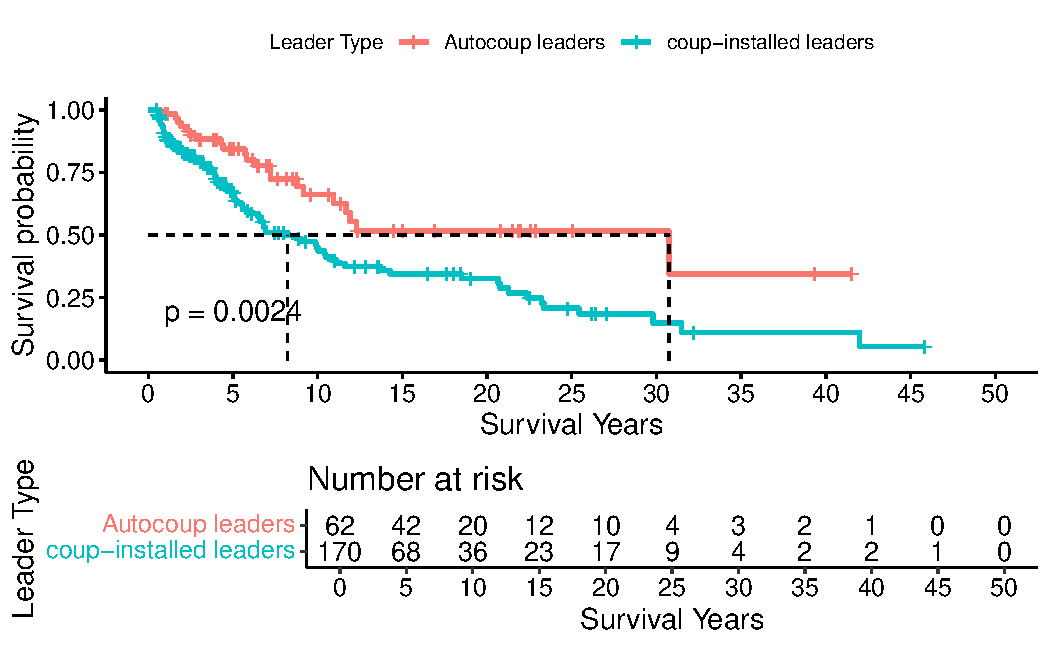
\includegraphics[keepaspectratio]{_coups_and_autocoups_correction_files/figure-pdf/fig-logrank-1.pdf}}

}

\caption{\label{fig-logrank}Survival Curves of Autocoup and
Coup-installed Leaders}

\end{figure}%

Preliminary survival analysis, as illustrated by the log-rank test in
Figure~\ref{fig-logrank}, reveals a statistically significant difference
in tenure length between coup-installed and autocoup leaders. The
survival curve for autocoup leaders consistently lies above that for
coup-installed leaders, suggesting both a lower hazard of removal and
longer durations in office for the former.

This study posits that the method of power acquisition plays a
significant role in determining leadership survival. Leaders installed
through coups may confront greater resistance or experience heightened
institutional fragility, thereby contributing to shorter average
tenures. Employing Cox proportional hazards and time-dependent Cox
models, the analysis supports this hypothesis by showing that autocoup
leaders tend to remain in office longer than their coup-installed
counterparts.

This research makes two principal contributions to the literature on
political survival. First, it introduces the mode of accession to power
as a previously under-explored explanatory factor. Second, through the
application of survival models, it provides robust empirical evidence of
the significant disparities in tenure between autocoup and
coup-installed leaders. These findings may help explain the increasing
prevalence of autocoup-driven tenure extensions since the early 2000s,
as incumbents observe and emulate the apparent success of prior cases.

The remainder of this chapter is organised as follows: Section 2 reviews
the relevant literature on political survival, establishing the
theoretical framework for the analysis. Section 3 explores the key
factors that influence the tenure of coup-installed and autocoup
leaders. Section 4 outlines the methodological approach and data
sources, with particular emphasis on survival analysis techniques.
Section 5 presents the empirical findings and discusses their
implications. Finally, Section 6 offers concluding reflections and
considers the broader significance of the findings for political
stability and democratic development.

\section{Literature review}\label{literature-review}

The longevity of political leaders, which varies markedly across
regimes, countries, and historical periods, has long been a focal point
of inquiry within political science. Research in this field is generally
categorised into two interrelated strands: regime survival and
individual leader survival. While the former concerns the endurance of
political systems---such as monarchies, dominant parties, or ideological
frameworks---the latter focuses on the duration of individual leaders'
tenure in office.

Patterns of political survival differ significantly across regime types.
For instance, parliamentary democracies (e.g., Japan and the United
Kingdom) often witness sustained party dominance alongside frequent
leadership turnover. Similarly, communist regimes (e.g., China) are
typically characterised by stable party control but relatively frequent
changes in leadership. In contrast, presidential systems (e.g., the
United States) and many military regimes tend to exhibit more frequent
changes in both leadership and ruling entity.

The existing literature on leader survival is both extensive and
diverse. Some studies investigate mechanisms that influence leadership
durability within specific regime types, such as democracies
(\citeproc{ref-svolik2014}{Svolik 2014}) or autocracies
(\citeproc{ref-davenport2021}{Davenport, RezaeeDaryakenari, and Wood
2021}). Others attempt to formulate more general theoretical frameworks
applicable across various political systems
(\citeproc{ref-buenodemesquita2003}{Bueno de Mesquita et al. 2003}).
Despite these efforts, the ambition of constructing a universal theory
of leadership survival remains elusive due to the inherent complexities
across regime contexts.

Mechanisms of leadership transition vary substantially between
democracies and autocracies. In autocratic regimes, leadership selection
processes are often closed, with access restricted to a limited elite.
Even when elections are held, meaningful competition is frequently
constrained by structural or legal barriers. The opacity of leadership
transitions in autocracies complicates assessments of popular support
and renders concepts such as selectorates or winning coalitions, as
theorised by Bueno de Mesquita et al.
(\citeproc{ref-buenodemesquita2003}{2003}), difficult to operationalise.

Given these challenges, focusing research on specific categories of
leaders may yield more analytically fruitful outcomes. The study of
irregular leaders---those who ascend to power via coups or extend their
rule through autocoups---offers a compelling line of inquiry due to the
distinctive uncertainty and volatility that characterise their tenures.

Two dominant perspectives have emerged in the literature to explain
leader survival. The first emphasises objective structural factors and
material resources, such as individual competence
(\citeproc{ref-yu2016}{Yu and Jong-A-Pin 2016}), societal stability
(\citeproc{ref-arriola2009}{Arriola 2009}), economic development
(\citeproc{ref-palmer1999}{Palmer and Whitten 1999};
\citeproc{ref-williams2011}{Williams 2011}), natural resource wealth
(\citeproc{ref-smith2004}{Smith 2004};
\citeproc{ref-quirozflores2012}{Quiroz Flores and Smith 2012};
\citeproc{ref-wright2013}{Wright, Frantz, and Geddes 2013}), and
external support (\citeproc{ref-licht2009}{Licht 2009};
\citeproc{ref-wright2008}{Wright 2008}; \citeproc{ref-thyne2017}{C.
Thyne et al. 2017}). The second perspective focuses on subjective
dimensions and strategic choices, including policy decisions, management
of opposition, and mechanisms for consolidating authority
(\citeproc{ref-gandhi2007}{Gandhi and Przeworski 2007};
\citeproc{ref-morrison2009}{Morrison 2009};
\citeproc{ref-escribuxe0-folch2013}{Escribà-Folch 2013};
\citeproc{ref-davenport2021}{Davenport, RezaeeDaryakenari, and Wood
2021}).

Coups, a critical form of irregular leadership transition, have garnered
substantial scholarly attention. Research has examined strategies for
coup prevention (\citeproc{ref-powell2017}{J. Powell 2017};
\citeproc{ref-sudduth2017}{Sudduth 2017}; \citeproc{ref-debruin2020}{De
Bruin 2020}), as well as the effects of coups on leadership trajectories
and the subsequent behaviour of coup leaders
(\citeproc{ref-sudduth2017}{Sudduth 2017};
\citeproc{ref-sudduth2018}{Sudduth and Bell 2018};
\citeproc{ref-easton2018}{Easton and Siverson 2018}).

Despite this body of work, a significant lacuna remains in the
comparative analysis of leadership survival between coup-installed and
autocoup leaders. This study seeks to address this gap by examining and
comparing the tenure lengths of leaders emerging from these two distinct
forms of irregular power acquisition.

By centring its analysis on the survival of coup-installed versus
autocoup leaders, this research aims to enhance our understanding of
political longevity in the context of irregular leadership transitions.
Such a focus promises to yield important insights into the strategic and
structural conditions that underpin leadership durability in diverse
political environments.

\section{Survival dynamics of autocoup and coup-installed
leaders}\label{survival-dynamics-of-autocoup-and-coup-installed-leaders}

The study of leadership survival within political systems poses
significant methodological and conceptual challenges, owing to the
opaque and complex nature of power transitions. These very challenges,
however, underscore the importance of such inquiry, as it illuminates
the often-neglected dynamics of political leadership. While the survival
trajectories of individual leaders vary considerably, discernible
patterns can be identified. Leaders emerging from similar origins or
operating within comparable regime types frequently display analogous
characteristics, thereby enabling systematic and meaningful comparative
analysis.

\subsection*{Key definitions and scope}\label{key-definitions-and-scope}
\addcontentsline{toc}{subsection}{Key definitions and scope}

Prior to undertaking a comparative analysis, it is essential to
establish clear definitions of key terms to ensure conceptual clarity
and analytical coherence. The definitions employed in this chapter align
with those presented in Chapter 2.

Autocoup leaders are defined as incumbent rulers who utilise
extra-constitutional measures to prolong their tenure in office. In
contrast, coup-installed leaders are those who ascend to power following
a successful coup, irrespective of whether they personally orchestrated
or participated in the coup. This inclusive definition encompasses both
coup perpetrators and individuals subsequently appointed to lead,
thereby offering a comprehensive perspective on leadership following
violent or forceful regime change.

Three clarifications are warranted in delineating the analytical scope.
First is about the minimum tenure threshold. To facilitate a meaningful
and robust analysis, the study imposes a minimum threshold of six months
in office for both autocoup and coup-installed leaders. This criterion
serves to exclude brief or interim leadership episodes that are less
analytically relevant to the study of survival dynamics, thereby
enhancing the reliability of the findings.

Second is the potential overlap in leadership categories. Some cases may
present ambiguities due to overlapping leadership pathways. A notable
example is Zine El Abidine Ben Ali, who assumed the presidency of
Tunisia in 1987 following a bloodless coup that removed President Habib
Bourguiba on grounds of ill health. In 2002, Ben Ali further
consolidated power through a constitutional referendum that removed term
limits and raised the presidential age cap from 70 to 75 years
(\citeproc{ref-bonci2019}{Bonci and Cavatorta 2019}). This latter
manoeuvre could be construed as an autocoup. Nevertheless, since Ben Ali
initially came to power via the 1987 coup and remained in office
continuously, he is classified in this study as a coup-installed leader.
To preserve analytical consistency and prevent category overlap, this
study adopts the rule that any leader who initially acquires office
through a coup is categorised as coup-installed, even if they later
consolidate or extend their rule through elections or
extra-constitutional means.

Third is the focus on post-event tenure. The analysis compares the
post-autocoup tenure of autocoup leaders with the post-coup tenure of
coup-installed leaders. Any period served by autocoup leaders prior to
the tenure-extending manoeuvre is excluded. This approach ensures a
like-for-like comparison by focusing on the period of leadership
characterised by irregular legitimacy and heightened political
uncertainty. Both categories of leaders share key characteristics---such
as limited institutional legitimacy, increased exposure to instability,
and dependence on coercive or extra-legal mechanisms---which render the
comparison analytically fruitful.

\subsection*{Challenges in power
consolidation}\label{challenges-in-power-consolidation}
\addcontentsline{toc}{subsection}{Challenges in power consolidation}

Both autocoup and coup-installed leaders encounter distinct challenges
in consolidating power, largely arising from the differing intensity of
issues related to illegitimacy, uncertainty, and instability. These
disparities create an uneven political landscape, placing coup-installed
leaders at a marked disadvantage. Table~\ref{tbl-leaders} presents a
comparative overview of the principal characteristics of autocoup and
coup-installed leaders, highlighting these critical differences.

\blandscape

\begin{table}

\caption{\label{tbl-leaders}Main Features of Autocoup and Coup-installed
Leaders}

\centering{

\fontsize{12.0pt}{14.4pt}\selectfont
\begin{tabular*}{1\linewidth}{@{\extracolsep{\fill}}>{\raggedright\arraybackslash}p{\dimexpr 112.50pt -2\tabcolsep-1.5\arrayrulewidth}>{\raggedright\arraybackslash}p{\dimexpr 225.00pt -2\tabcolsep-1.5\arrayrulewidth}>{\raggedright\arraybackslash}p{\dimexpr 225.00pt -2\tabcolsep-1.5\arrayrulewidth}}
\toprule
Feature & Autocoup Leader & Coup Entry Leader \\ 
\midrule\addlinespace[2.5pt]
Illegitimacy & Normally attained through
lawful procedures, but
lacking consensus
legitimacy & Blatantly illegal \\ 
Uncertainty & Initially with some certainty, but decreases as the leader's age grows or health worsens & Significant uncertainty initially \\ 
Instability & Relatively stable & Unstable except when a strongman emerges or constitutional institutions are established \\ 
Balance of Power & Generally in a better position of power & Initially unclear and challenging to establish a balance \\ 
\bottomrule
\end{tabular*}

}

\end{table}%

\elandscape

\subsubsection*{Illegitimacy}\label{illegitimacy}
\addcontentsline{toc}{subsubsection}{Illegitimacy}

Although both categories of leaders face legitimacy deficits, the nature
and perception of this deficit vary considerably.

For coup-installed leaders, illegitimacy is overt and unequivocal,
stemming from the direct---often violent---seizure of power. Such abrupt
disruptions to established political norms and institutions elicit
immediate condemnation, both domestically and internationally, and cast
doubt on the regime's authority from the outset.

By contrast, autocoup leaders adopt a more covert and strategic
approach, utilising legal and institutional mechanisms to lend a veneer
of democratic legitimacy. Though often superficial, this legalistic
veneer can obscure the authoritarian nature of their actions, offering a
temporary shield from domestic opposition and international scrutiny
while they seek to consolidate power.

\subsubsection*{Uncertainty}\label{uncertainty}
\addcontentsline{toc}{subsubsection}{Uncertainty}

The irregular accession of both types of leaders generates uncertainty
regarding the durability of their rule and the modalities of succession.
However, the nature and sources of this uncertainty differ markedly.

Coup-installed leaders confront a triad of uncertainties. First, the
immediate post-coup environment frequently involves intense power
struggles within the military or ruling coalition, creating ambiguity
over who will ultimately prevail. Second, their tenure is intrinsically
unstable, threatened by internal rivalries, popular mobilisation, or the
prospect of counter-coups. Third, the absence of institutionalised
succession mechanisms exacerbates this unpredictability, heightening the
risk of future instability.

Autocoup leaders, while not entirely insulated from uncertainty,
typically face fewer ambiguities. As incumbents, they retain formal
authority post-autocoup, thereby eliminating immediate succession
questions. Moreover, autocoup leaders often articulate explicit
ambitions to prolong their rule indefinitely, or through gradual
extensions, cultivating an image of continuity. This perceived
stability---whether genuine or contrived---may foster a more predictable
political climate in the short term.

\subsubsection*{Instability}\label{instability}
\addcontentsline{toc}{subsubsection}{Instability}

The combination of legitimacy deficits and enduring uncertainty
inevitably fosters insecurity and a sense of political fragility.
Consequently, both autocoup and coup-installed leaders prioritise
strategies to stabilise their regimes. However, the scale and nature of
these challenges differ.

Coup-installed leaders typically face the formidable task of
reconfiguring political power from the ground up. This often involves
purging opponents, suppressing dissent, and restructuring institutional
frameworks. Such aggressive measures can provoke significant resistance,
alienate potential allies, and incite societal unrest. Moreover, the
imperative to appease powerful domestic and international actors may
force these leaders into precarious compromises that further undermine
their authority.

In contrast, autocoup leaders often benefit from a degree of
institutional continuity and regime loyalty. This relative stability
enables them to pursue consolidation incrementally, reducing the
likelihood of immediate backlash. While opposition may persist, autocoup
leaders are generally less exposed to existential threats in the early
stages of their extended rule, affording them greater latitude to
entrench their authority.

Understanding these contrasting challenges allows for a more refined
appreciation of the strategic environments in which irregular leaders
operate. This comparative lens provides a valuable framework for
analysing the divergent pathways to power consolidation, and the varied
tools and tactics employed by autocoup and coup-installed leaders in
navigating the precarious terrain of non-traditional political
ascension.

\subsection*{Empirical evidence and
hypothesis}\label{empirical-evidence-and-hypothesis}
\addcontentsline{toc}{subsection}{Empirical evidence and hypothesis}

Empirical evidence underscores the relative disadvantage faced by
coup-installed leaders, revealing a complex interplay between historical
patterns, difficulties in consolidating power, and variations in
leadership longevity. This section presents key empirical findings and
introduces the central hypothesis that guides this study.

Data analysis indicates a strong correlation between the frequency of
coup attempts within a given country and the likelihood of future coups.
Notably, more than one-third of all coups since 1950 have taken place in
the ten countries with the highest number of coup attempts
(\citeproc{ref-powell2011}{Powell and Thyne 2011}). This suggests a
self-reinforcing cycle of political instability, in which each
successful coup increases the probability of further attempts, thereby
cultivating an environment of persistent uncertainty for coup-installed
leaders.

The disparity in leadership duration between autocoup and coup-installed
leaders is clearly reflected in survival data. As illustrated in
Figure~\ref{fig-logrank}, leaders who extend their tenure through
autocoups remain in office, on average, approximately five years longer
than those who assume power via coups. This marked difference in tenure
highlights the distinct challenges these two categories of leaders
encounter in retaining power.

The divergent consolidation environments faced by autocoup and
coup-installed leaders contribute to a self-perpetuating cycle with
significant implications for tenure length. Coup-installed leaders
confront acute legitimacy deficits and heightened internal instability;
they often struggle to attract and retain durable support, rendering
them more susceptible to both internal dissent and external pressures.
Their comparatively shorter average tenures reinforce perceptions of
volatility and fragility. Autocoup leaders, by contrast, frequently
benefit from a superficial veneer of legality and enjoy a more
favourable starting position as incumbents. This allows them to
consolidate authority more effectively, cultivate elite and public
support, and reduce the immediate risk of displacement. Their longer
tenures further contribute to perceptions of regime stability. This
cyclical dynamic suggests that the initial method of acquiring or
extending power has long-term implications for a leader's capacity to
maintain their position.

Drawing upon these empirical observations and the theoretical framework
outlined in preceding sections, the following hypothesis is proposed:

\textbf{\emph{H4-1: Political leaders who successfully extend their
tenure through autocoups are more likely to enjoy longer extended
tenures than those who assume office through coups.}}

This hypothesis encapsulates the anticipated effects of the differing
challenges and advantages faced by coup-installed and autocoup leaders.
By empirically testing this claim, the study seeks to assess the impact
of irregular accession mechanisms on leadership survival, thereby
advancing a more nuanced understanding of political durability in
contexts of non-traditional transitions to power.

\section{Research design}\label{research-design-1}

This section outlines the methodological framework employed to test the
hypothesis that autocoup leaders exhibit longer survival times in office
than coup-installed leaders. Survival analysis is utilised to model
leadership tenure, with Cox proportional hazards models employed to
estimate the effects of leader type while controlling for relevant
covariates.

\subsection*{Methodology: Survival
analysis}\label{methodology-survival-analysis}
\addcontentsline{toc}{subsection}{Methodology: Survival analysis}

Two variants of the Cox model are employed to analyse the survival
durations of coup-installed and autocoup leaders.

\textbf{Cox proportional hazards (PH) model}: This model incorporates
only time-invariant covariates measured at the time of the leader's
entry into office. It assumes that the effects of these covariates on
the hazard rate remain constant over time.

\textbf{Time-dependent Cox model}: This model allows for the inclusion
of covariates whose values may vary over time, such as indicators of
economic performance and levels of political violence. By incorporating
temporal variation, this model offers a more dynamic and nuanced
analysis of leadership survival.

The Cox model is preferred over the Kaplan-Meier estimator due to its
capacity to account for multiple explanatory variables simultaneously.
Although the Cox model does not directly estimate the expected duration
of tenure, it estimates the hazard ratio, which reflects the relative
risk of being removed from office. A higher cumulative hazard
corresponds to a lower probability of survival, thereby capturing
critical dynamics of leadership vulnerability over time.

\subsection*{Data and variables}\label{data-and-variables-1}
\addcontentsline{toc}{subsection}{Data and variables}

The analysis relies on a set of dependent and independent variables,
complemented by a range of controls.

\textbf{Survival Time:} Measured in days, this variable captures the
length of a leader's tenure. For coup-installed leaders, the tenure is
measured from the date of their accession via coup. For autocoup
leaders, it begins on the date their original legitimate term would have
expired. For instance, Vladimir Putin assumed the presidency of Russia
in 2000, stepped down in 2008 after completing two terms, and assumed
the post of prime minister while continuing to exert de facto control.
His post-autocoup tenure, therefore, is coded as beginning in 2008.

\textbf{End Point Status:} This categorical variable indicates how a
leader's tenure ended:

\begin{itemize}
\item
  \textbf{0 = Censored:} Denotes leaders who exited office through
  regular or voluntary means, such as electoral defeat, term expiration,
  voluntary resignation due to health, or natural death.
\item
  \textbf{1 = Ousted:} Denotes leaders who were forcibly removed,
  including through coups, resignations under pressure, or
  assassination.
\end{itemize}

The key independent variable is the leader type, which categorizes
leaders into two distinct groups:

\begin{itemize}
\tightlist
\item
  \textbf{Group A = Non-coup leader}: A leader who assumes power through
  regular means.
\item
  \textbf{Group B = Autocoup leader}: An incumbent who extends their
  tenure through extra-constitutional means.
\item
  \textbf{Group C = Coup-installed leader}: A leader who assumes power
  through a coup, whether or not they personally participated in its
  execution.
\end{itemize}

This variable serves as the primary explanatory factor, enabling a
direct comparison of survival outcomes between the two categories of
irregular leaders.

Data for the dependent and independent variables are drawn from the
newly constructed autocoup dataset introduced in this study, as well as
the Archigos dataset (\citeproc{ref-goemans2009}{Goemans, Gleditsch, and
Chiozza 2009})and the Political Leaders and Alliances Dataset (PLAD)
(\citeproc{ref-bomprezzi2024wedded}{Bomprezzi et al. 2024}).

To isolate the effect of leader type on survival, the analysis
incorporates a set of control variables, as identified in the autocoup
analysis presented in Chapter 3. Among these are regime
type---categorised as democracy, hybrid regime, or autocracy---to
account for institutional differences that may influence leadership
stability; economic performance, measured through macroeconomic
indicators such as GDP growth, which may affect a leader's ability to
retain support; political violence, which captures the extent of civil
conflict, repression, or unrest that can threaten regime stability and
leadership tenure; population size, to control for structural
differences across states that may impact political dynamics; and Polity
V scores, which reflect the institutional characteristics and the degree
of democracy or autocracy within a regime.These control variables
enhance the comparability and robustness of the statistical models,
ensuring that the estimated effects of leader type are not confounded by
broader political, economic, or demographic conditions.

\section{Results and discussion}\label{results-and-discussion-1}

\subsection*{Model results}\label{model-results}
\addcontentsline{toc}{subsection}{Model results}

Regression estimates from both the Cox Proportional Hazards (PH) model
and the time-dependent Cox model---calculated using the survival package
in R (\citeproc{ref-survival}{Therneau 2024})---are presented in
Table~\ref{tbl-cox}. These two model specifications produce divergent
findings with respect to the central question of this study: whether the
method of power acquisition significantly affects the survival prospects
of political leaders.

\begin{table}

\caption{\label{tbl-cox}Cox Models for Survival Time of Different Types
of Leaders}

\centering{

\fontsize{9.8pt}{11.7pt}\selectfont
\begin{tabular*}{\linewidth}{@{\extracolsep{\fill}}lcccccccc}
\toprule
 & \multicolumn{4}{c}{\textbf{Cox PH Model}} & \multicolumn{4}{c}{\textbf{Time-dependent Cox Model}} \\ 
\cmidrule(lr){2-5} \cmidrule(lr){6-9}
\textbf{Characteristic} & \textbf{N} & \textbf{Event N} & \textbf{HR}\textsuperscript{\textit{1}} & \textbf{SE} & \textbf{N} & \textbf{Event N} & \textbf{HR}\textsuperscript{\textit{1}} & \textbf{SE} \\ 
\midrule\addlinespace[2.5pt]
{\bfseries Leader Type} &  &  &  &  &  &  &  &  \\ 
    Non-coup leaders & 1,506 & 195 & 1.00 & — & 8,039 & 196 & 1.00 & — \\ 
    Autocoup leaders & 58 & 20 & 1.21 & 0.247 & 507 & 20 & 1.22 & 0.244 \\ 
    Coup-installed leaders & 152 & 75 & 1.77*** & 0.155 & 998 & 75 & 1.26 & 0.170 \\ 
{\bfseries Regime Types} &  &  &  &  &  &  &  &  \\ 
    Dominant-party & 267 & 68 & 1.00 & — & 2,610 & 63 & 1.00 & — \\ 
    Military & 138 & 51 & 2.64*** & 0.194 & 656 & 60 & 3.17*** & 0.213 \\ 
    Personal & 137 & 61 & 1.70*** & 0.181 & 1,551 & 82 & 1.78*** & 0.175 \\ 
    Presidential & 346 & 42 & 1.42 & 0.229 & 1,819 & 39 & 1.31 & 0.269 \\ 
    Parliamentary & 711 & 35 & 1.29 & 0.245 & 2,555 & 31 & 1.28 & 0.292 \\ 
    Other & 117 & 33 & 2.27*** & 0.226 & 353 & 16 & 2.10** & 0.302 \\ 
{\bfseries GDP Growth Trend} & 1,716 & 290 & 0.62 & 0.984 & 9,544 & 291 & 0.13*** & 0.782 \\ 
{\bfseries GDP per capita} & 1,716 & 290 & 0.96*** & 0.008 & 9,544 & 291 & 0.96*** & 0.007 \\ 
{\bfseries Population: log} & 1,716 & 290 & 0.99 & 0.043 & 9,544 & 291 & 0.96 & 0.044 \\ 
{\bfseries Polity V score} & 1,716 & 290 & 0.98* & 0.013 & 9,544 & 291 & 0.99 & 0.015 \\ 
{\bfseries Political violence} & 1,716 & 290 & 0.98 & 0.030 & 9,544 & 291 & 1.06** & 0.027 \\ 
\bottomrule
\end{tabular*}
\begin{minipage}{\linewidth}
\textsuperscript{\textit{1}}*p\textless{}0.1; **p\textless{}0.05; ***p\textless{}0.01\\
Abbreviations: HR = Hazard Ratio, SE = Standard Error\\
\end{minipage}

}

\end{table}%

The Cox PH model identifies a statistically significant difference in
the hazard of removal between coup-installed and non-coup leaders.
Specifically, coup-installed leaders face a hazard ratio of 1.77
relative to non-coup leaders (p \textless{} 0.01), suggesting they are
significantly more likely to be ousted. In contrast, autocoup leaders
exhibit a hazard ratio of 1.21, which does not reach statistical
significance. However, the time-dependent Cox model---which accounts for
time-varying covariates such as economic performance and political
violence---does not reveal any statistically significant difference in
removal risk between leader types. The hazard ratios for both autocoup
(1.22) and coup-installed (1.26) leaders are statistically
indistinguishable from unity when compared to the non-coup baseline.
This is also true when take the coup-installed leaders as the reference,
which shows no significant difference among these three groups of
leaders.

Given the superior robustness of the time-dependent model in accounting
for evolving political and economic conditions, the principal
interpretation of the findings rests on this specification. Contrary to
the initial hypothesis, and despite preliminary evidence from simpler
models, the manner in which power is acquired---whether through a coup
or autocoup---does not independently predict leader survival once key
contextual variables are incorporated.

Instead, regime type emerges as the most significant predictor of
leadership survival. Leaders in military regimes exhibit a hazard ratio
of 3.17 (p \textless{} 0.01), indicating a \(217\%\) higher risk of
removal compared to leaders in dominant-party regimes. Similarly,
leaders in personalist regimes (HR = 1.78, p \textless{} 0.01) and in
regimes classified as ``Other'' (HR = 2.10, p \textless{}
0.05)---including transitional or provisional arrangements---are also
significantly more vulnerable. These results suggest that institutional
fragility, factionalism, and weak legitimacy associated with such regime
types substantially increase the likelihood of leadership turnover.

Economic conditions also play a noteworthy role. GDP per capita exhibits
a negative and statistically significant relationship with leader
removal (HR = 0.96, p \textless{} 0.01), indicating that greater
economic development corresponds with increased political stability. In
practical terms, each additional \$10,000 in GDP per capita reduces the
hazard of removal by approximately \(4\%\), all else equal. Furthermore,
GDP growth trends are strongly associated with survival (HR = 0.13, p
\textless{} 0.01), suggesting that sustained economic performance
significantly enhances leader durability, each 1 point increase of GDP
growth ( \(1\%\) GDP growth over the average growth rate for the
previous 5 years) reduces the hazard of removal by approximately
\(87\%\), all else equal.

Conversely, political violence emerges as a destabilising force. A
one-unit increase in the political violence index raises the hazard of
removal by approximately \(6\%\) (HR = 1.06, p \textless{} 0.05),
underscoring the impact of societal unrest and conflict on the
sustainability of political leadership.

Other variables, such as population size (log-transformed) and Polity V
scores, do not attain statistical significance in the time-dependent
model. While these measures are often cited as important predictors of
regime stability and institutional quality, their limited explanatory
power in this context implies that more proximate factors---such as
regime structure and active conflict---play a more immediate role in
shaping survival outcomes following irregular accessions to power.

It is important to highlight that these results are conditional upon the
exclusion of leaders who remained in office for fewer than 180 days
after their initial seizure of power. This exclusion is analytically
justified, given that many such short-lived leaders---particularly those
emerging from failed coups---do not manage to consolidate authority and
are therefore ill-suited for meaningful survival analysis. Including
these cases could artificially inflate the hazard ratios for
coup-installed leaders, thereby skewing the results.

In sum, this study finds limited support for the hypothesis that
autocoup leaders enjoy greater tenure than their coup-installed
counterparts. Instead, it confirms that broader structural and
institutional conditions---especially regime type and socio-economic
context---are the primary determinants of leadership survival following
irregular accessions to power.

\subsection*{Discussion}\label{discussion}
\addcontentsline{toc}{subsection}{Discussion}

\begin{figure}

\begin{minipage}{0.50\linewidth}

\centering{

\pandocbounded{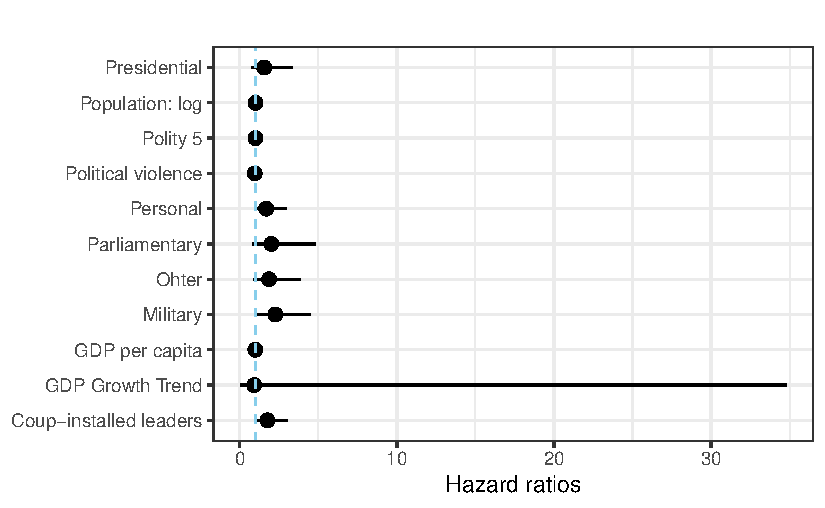
\includegraphics[keepaspectratio]{_coups_and_autocoups_correction_files/figure-pdf/fig-coxHR-1.pdf}}

}

\subcaption{\label{fig-coxHR-1}Cox PH Model}

\end{minipage}%
%
\begin{minipage}{0.50\linewidth}

\centering{

\pandocbounded{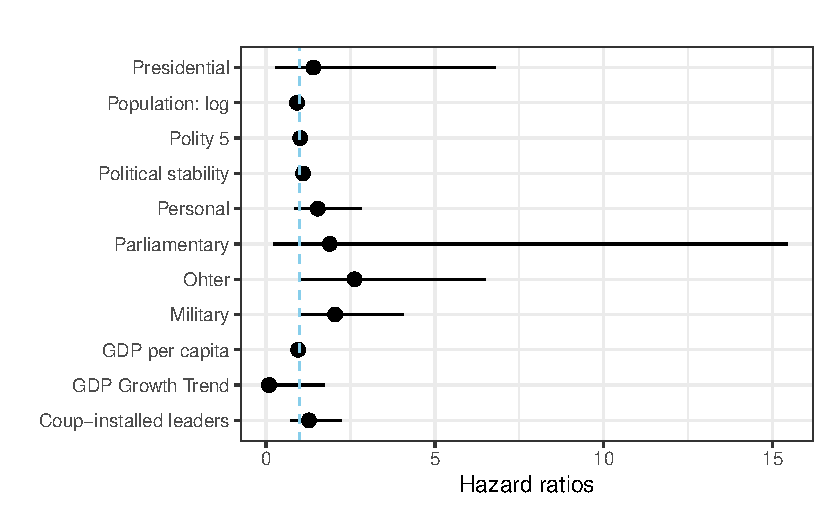
\includegraphics[keepaspectratio]{_coups_and_autocoups_correction_files/figure-pdf/fig-coxHR-2.pdf}}

}

\subcaption{\label{fig-coxHR-2}Time-dependent Cox Model}

\end{minipage}%

\caption{\label{fig-coxHR}Hazard Ratios and 95\% CIs for Leader Ousting}

\end{figure}%

Figure~\ref{fig-coxHR} presents the hazard ratios (HRs) and their
corresponding \(95\%\) confidence intervals for the covariates included
in the Cox Proportional Hazards (PH) model (left panel) and the
time-dependent Cox model (right panel). Each dot represents the
estimated hazard ratio, while the horizontal lines denote the \(95\%\)
confidence intervals. A hazard ratio of 1 indicates no effect on the
probability of removal from office. Variables whose confidence intervals
cross the vertical dashed blue line at 1 are not statistically
significant at the \(5\%\) level. Given its ability to account for
time-varying covariates and evolving structural conditions, the
time-dependent Cox model provides the principal basis for
interpretation.

While the effect of leadership type varies across models, the
time-dependent Cox model---on which the principal interpretation is
based---shows that neither coup-installed nor autocoup leaders have a
statistically significant impact on survival tenure. In this
specification, the confidence intervals for both categories cross the
reference line, indicating that once relevant covariates are controlled
for, the mode of accession does not independently influence the hazard
of removal.

In contrast, regime type emerges as a robust determinant of political
survival. Leaders operating within military regimes, personalist
regimes, and those classified under ``Other'' regime types (typically
transitional or provisional governments) face markedly elevated hazards
of removal. The hazard ratios for these categories are significantly
greater than 1 and attain statistical significance at the \(5\%\) level,
signalling a consistently heightened vulnerability. This aligns with the
broader theoretical contention that regime institutionalisation and
coherence are central to leadership stability.

Conversely, the effects associated with more democratic regime
types---parliamentary and presidential systems---while positive, do not
reach statistical significance. Their confidence intervals intersect the
reference line, suggesting that, under conditions of irregular
accession, the institutional architecture of democratic regimes may not
offer immediate protective advantages to incumbents.

Economic performance plays a meaningful role. GDP growth exhibits a
pronounced and statistically significant negative effect on the hazard
of removal. The associated hazard ratio is considerably below 1 and lies
far from the reference line, suggesting that improved economic
performance substantially reduces the likelihood of political removal.
GDP per capita is also statistically significant, though its hazard
ratio is very close to 1, implying only a modest substantive effect.
These findings reinforce the well-established association between
economic stability and political survival.

Political violence also shows a statistically significant effect, but
with a hazard ratio close to 1, indicating that while it increases the
risk of removal, its magnitude is limited. Similarly, other control
variables such as population size (logged) and Polity V scores fail to
achieve statistical significance. Their estimated hazard ratios are near
1 and their confidence intervals encompass the reference line. This
suggests that these structural and institutional indicators, though
theoretically important, exert minimal influence on short- to
medium-term leadership survival in the context of irregular accession.

These findings collectively reinforce the argument that, in the
aftermath of irregular leadership transitions, regime context and
dynamic political-economic conditions are more consequential for tenure
than the specific mode of accession. While the method of taking
power---coup versus autocoup---may matter symbolically or normatively,
it is the surrounding regime environment and its capacity to manage
threats, maintain coherence, and deliver stability that ultimately
determine political longevity.

\subsection*{Assessing the proportional hazards
assumption}\label{assessing-the-proportional-hazards-assumption}
\addcontentsline{toc}{subsection}{Assessing the proportional hazards
assumption}

Evaluating the proportional hazards assumption is a critical step in
validating the reliability of estimates produced by the Cox regression
models. This assumption was tested using a chi-squared test based on
Schoenfeld residuals, which assesses whether the effect of each
covariate remains constant over time. The test results indicate that the
assumption is not violated in either the standard Cox Proportional
Hazards (PH) model or the time-dependent Cox model. The global
p-values---0.12 for the standard model and 0.23 for the time-dependent
model---both exceed the conventional \(5\%\) significance threshold,
thereby confirming that the proportional hazards assumption is satisfied
in both cases.

\section{Summary}\label{summary-2}

This chapter has explored the survival prospects of political leaders
who assumed office through irregular means---specifically via coups and
autocoups---using survival analysis techniques, including the Cox
Proportional Hazards model and a time-dependent Cox model. While the
standard Cox model identified a statistically significant difference in
removal risk between coup-installed and non-coup leaders, this effect
was not sustained in the more rigorous time-dependent model. Once
time-varying covariates were accounted for, the mode of power
acquisition---whether through a coup or an autocoup---did not
independently predict leadership duration.

The principal findings suggest that leadership type is not a significant
determinant of political survival when contextual variables such as
regime type, economic performance, and political violence are
considered. In particular, regime type consistently emerges as the most
influential factor. Leaders in military, personalist, and transitional
(``other'') regimes face significantly higher hazards of removal than
those in dominant-party systems, highlighting the institutional
instability and vulnerability associated with less consolidated
political structures.

Economic development also plays an important role. Higher levels of GDP
per capita are associated with greater leadership stability, while GDP
growth exerts an especially strong effect: even modest increases in
growth rates substantially reduce the risk of removal. Conversely,
political violence increases the likelihood of ousting, underscoring the
destabilising impact of unrest and conflict on leader survival.

Other structural variables, such as population size and Polity V scores,
do not attain statistical significance in the time-dependent model.
Their limited effect in this context suggests that under conditions of
irregular accession, proximate and dynamic factors---particularly those
relating to regime structure and economic performance---are more
consequential than long-term institutional attributes.

Methodologically, this chapter illustrates the analytical value of
time-dependent survival models in capturing the effects of evolving
covariates. Substantively, it provides one of the first systematic
empirical investigations into the survival of autocoup leaders,
contributing to the growing literature on irregular leadership
transitions. While the newly constructed autocoup dataset represents a
valuable innovation, its limitations point to the need for further
refinement and expansion in future research.

In sum, this chapter finds that regime characteristics and economic
dynamics, rather than the mode of accession, are the principal
determinants of political survival following irregular transitions to
power. These findings contribute to broader debates on authoritarian
resilience, executive instability, and the structural foundations of
political longevity.

\chapter{Coups, Autocoups, and
Democracy}\label{coups-autocoups-and-democracy}

\section*{Abstract}\label{abstract-4}
\addcontentsline{toc}{section}{Abstract}

This chapter investigates the impact of autocoups on political
institutions, comparing them with traditional coups through an analysis
of variations in Polity V scores. It advances two primary hypotheses:
first, that incumbent leaders frequently consolidate power by
systematically undermining institutional constraints in the period
leading up to an autocoup, resulting in a decline in Polity V scores
attributable to the autocoup. Second, unlike traditional coups, which
exhibit a ``U-shaped'' trajectory in Polity V scores, autocoups
precipitate a persistent decline in these scores without subsequent
recovery. This is attributed to autocoup leaders' deliberate intent to
suppress opposition and dismantle institutional checks and balances to
secure prolonged tenure.

Employing a country-fixed effects model, this study demonstrates that
Polity V scores typically decline following autocoups, mirroring the
magnitude of decline observed after traditional coups. However, while
traditional coups often lead to an immediate reduction in Polity V
scores followed by conditions conducive to recovery over time, autocoups
result in sustained democratic erosion. These findings highlight the
divergent political trajectories induced by coups and autocoups.

This research addresses a critical gap in the empirical analysis of
autocoups and contributes to academic and policy discussion by
elucidating their detrimental effects, particularly in terms of
democratic backsliding and the entrenchment of authoritarian governance.

\newpage

\section{Introduction}\label{introduction-4}

Previous chapters have delineated the concept of an autocoup, introduced
a novel dataset documenting such events, conducted empirical analyses of
the determinants of autocoup attempts, and compared the post-event
survival durations of leaders installed by coups and autocoups. A
logical extension of this inquiry is to explore the broader implications
of autocoups, particularly their impact on democratisation processes
from a political science perspective.

The absence of a comprehensive, widely accepted dataset on autocoups has
historically limited discussion of their consequences to primarily
case-study-based analyses (\citeproc{ref-baturo2019politics}{Baturo and
Elgie 2019}; \citeproc{ref-baturo2022}{Baturo and Tolstrup 2022}). In
contrast, the impact of traditional coups on democratisation has been
extensively explored through empirical studies
(\citeproc{ref-powell2014a}{J. Powell 2014}; \citeproc{ref-thyne2014}{C.
Thyne and Powell 2014}; \citeproc{ref-derpanopoulos2016}{Derpanopoulos
et al. 2016}; \citeproc{ref-miller2016}{M. K. Miller 2016};
\citeproc{ref-dahl2023}{Dahl and Gleditsch 2023}). Although debates
persist, a significant body of literature suggests that coups may exert
a positive effect on democratisation over time.

To move beyond case-specific narratives and achieve a more systematic
and comparative understanding, this chapter undertakes the first
empirical investigation into the democratic consequences of autocoups.
Its primary objective is to determine whether autocoups entrench
authoritarian rule, facilitate democratisation, or have no substantive
impact on regime transitions.

Given the conceptual and empirical parallels between coups and
autocoups, a secondary aim is to compare their respective effects on
democratisation. While both phenomena disrupt established political
orders, their immediate and longer-term consequences may differ
markedly. Clarifying these distinctions is essential for assessing their
broader political ramifications.

To address these questions, this study utilises an established dataset
on coups alongside a newly constructed dataset on autocoups. Employing a
fixed-effects model, it evaluates their respective impacts on democratic
quality, operationalised through Polity V scores. The findings indicate
that both coups and autocoups are associated with an immediate decline
in democratic quality. However, while Polity V scores affected by coups
typically exhibit notable recovery within two years, those impacted by
autocoups show no such improvement over the same period.

This study makes two principal contributions to political science.
First, it provides the first empirical analysis of the impact of
autocoups on democratisation, thereby addressing a significant gap in
the literature. Second, by comparing the effects of coups and
autocoups---and demonstrating the more severe and sustained damage to
democratic institutions caused by the latter---it underscores the need
to treat autocoups as a distinct political phenomenon warranting greater
scholarly and policy attention.

The remainder of this chapter is structured as follows. Section 2
examines the impact of autocoups on democratisation, with particular
emphasis on their comparison with traditional coups. Section 3 outlines
the research design, methodological approach, and variables employed.
Section 4 presents the empirical findings and discusses their broader
implications. Section 5 concludes by summarising the key findings and
reflecting on their significance for understanding and addressing
autocoup dynamics.

\section{Impact of autocoups on political
change}\label{impact-of-autocoups-on-political-change}

As outlined in Chapter 2, an autocoup refers to a situation in which an
incumbent leader extends their tenure beyond constitutionally mandated
limits through extra-constitutional means. While the official title or
institutional framework may be altered, the individual wielding
political power remains the same. In contrast to traditional coups,
autocoups do not result in genuine leadership turnover, elite
restructuring, or fundamental regime transformation; the core structure
of rule persists.

This distinction has important implications. Because regime change
seldom follows a successful autocoup, its political effects cannot be
adequately captured through conventional analytical frameworks. Most
studies on coups and democratisation assess outcomes in terms of regime
transitions---from autocracy to democracy or vice versa---as seen in
prior research (\citeproc{ref-thyne2014}{C. Thyne and Powell 2014};
\citeproc{ref-derpanopoulos2016}{Derpanopoulos et al. 2016};
\citeproc{ref-miller2016}{M. K. Miller 2016}). However, such binary
frameworks are ill-suited for analysing autocoups, which rarely
precipitate formal regime change.

Nevertheless, the absence of regime transition does not imply political
continuity or stasis. On the contrary, autocoups frequently reshape
political dynamics and can trigger substantial institutional and
behavioural changes. Accordingly, a more appropriate approach for
assessing their political impact is to examine changes in democracy
indices, such as those provided by the Polity5 dataset
(\citeproc{ref-p1}{Monty G. Marshall and Gurr 2020}). The Polity V
score, which ranges from −10 (full autocracy) to +10 (full democracy),
allows for the identification of incremental shifts in democratic
institutions and constraints on executive power, even in the absence of
formal regime turnover. This methodological approach is consistent with
recent studies (\citeproc{ref-dahl2023}{Dahl and Gleditsch 2023}).

Although autocoups rarely result in overt regime transformation, their
implications for democratisation are considerable. In particular, their
negative effects appear to be more severe and enduring than those
associated with traditional coups.

\subsection*{Immediate democratic backsliding following
autocoups}\label{immediate-democratic-backsliding-following-autocoups}
\addcontentsline{toc}{subsection}{Immediate democratic backsliding
following autocoups}

Unlike coups---which are typically characterised by abrupt disruptions
such as the removal of a sitting leader---autocoups often unfold
gradually. Incumbents seeking to extend their tenure usually undertake
preparatory measures well in advance of the decisive act. These measures
may include purging political elites, suppressing opposition parties,
repressing protest movements, and restricting media freedoms. In the
absence of such groundwork, an autocoup would likely face formidable
resistance and may fail. As a result, democratic decline often begins
prior to the formal execution of the autocoup, with Polity V scores
reflecting deterioration during this preparatory phase.

One frequently cited case is Peru in 1992. President Alberto Fujimori
dissolved Congress, suspended the 1979 Constitution, and ruled by decree
until a new constituent assembly was elected to draft a revised
constitution (\citeproc{ref-cameron1998}{Maxwell A. Cameron 1998b}).
Although these actions did not immediately secure his continued
rule---given the constitutional prohibition on immediate
re-election---Fujimori's constitutional reforms in 1993 enabled him to
win a second term in 1995 (\citeproc{ref-baturo2019}{Baturo 2019}).

Polity V scores illustrate the political consequences of this process.
When Fujimori entered office in 1990, Peru's score stood at 8, where it
remained in 1991. Following the 1992 dissolution of Congress, the score
plummeted to −4. After the 1993 constitutional revision, the score rose
marginally to −1, where it remained throughout the rest of Fujimori's
presidency. This indicates that while there was a partial recovery in
institutional ratings, democratic quality never returned to pre-autocoup
levels.

A similar trajectory can be observed in Belarus under Alexander
Lukashenko. Upon taking office in 1994, Belarus received a Polity V
score of 8. However, after Lukashenko bypassed parliamentary opposition
through a controversial referendum in 1995, the score fell to 0.
Following a second referendum in 1996 that extended his presidential
term, the score dropped further to −7, where it has remained ever since,
despite additional term extensions (\citeproc{ref-ash2014}{Ash 2014};
\citeproc{ref-baturo2019politics}{Baturo and Elgie 2019}).

In contrast, traditional coups typically occur without prior access to
state institutions, and coup plotters are less able to prepare the
ground in advance. However, once in power, they often consolidate
authority swiftly by removing or neutralising previous officeholders and
political opponents (\citeproc{ref-pieterse1982}{Pieterse 1982}). This
may involve dissolving legislatures, suspending constitutions, or ruling
by decree or military command
(\citeproc{ref-onwumechili1998african}{Onwumechili 1998};
\citeproc{ref-miller2011debunking}{A. C. Miller 2011}). As a result,
traditional coups also lead to a decline in Polity V scores, though
through more immediate and disruptive mechanisms.

Based on the above discussion, the following hypothesis is proposed:

\textbf{\emph{H5-1: Autocoups will result in a significant decline in
Polity V scores immediately following their occurrence, in a manner
comparable to the effects observed in traditional coups.}}

\subsection*{Consistent outcomes of autocoups versus the ``U-shaped''
effects of
coups}\label{consistent-outcomes-of-autocoups-versus-the-u-shaped-effects-of-coups}
\addcontentsline{toc}{subsection}{Consistent outcomes of autocoups
versus the ``U-shaped'' effects of coups}

Over the longer term, in contrast to the more ambiguous and
context-dependent effects of traditional coups
(\citeproc{ref-dahl2023}{Dahl and Gleditsch 2023}), autocoups seldom
contribute to processes of democratisation.

The relationship between coups and democratisation has been extensively
examined in the scholarly literature. Some scholars argue that
coups---or even the credible threat of them---can act as catalysts for
democratic transitions. One line of reasoning suggests that coups may
generate a political ``shock'' that creates openings for liberalisation
which would not otherwise emerge (\citeproc{ref-thyne2014}{C. Thyne and
Powell 2014}). In a critical reassessment, Derpanopoulos et al.
(\citeproc{ref-derpanopoulos2016}{2016}) questioned the assumed
democratising potential of coups, prompting further empirical and
theoretical engagement, including a notable response by M. K. Miller
(\citeproc{ref-miller2016}{2016}). More recently, Dahl and Gleditsch
(\citeproc{ref-dahl2023}{2023}) has advanced this debate by suggesting
that the aftermath of coups can lead to either democratic or
authoritarian trajectories, largely depending on the extent and nature
of popular mobilisation.

A frequently cited example of a so-called ``pro-democracy coup'' is that
of Niger in February 2010, when the military removed President Mamadou
Tandja after he unconstitutionally extended his mandate. The Supreme
Council for the Restoration of Democracy (CSRD) assumed power and
committed to restoring constitutional rule. Their actions were welcomed
both domestically and internationally as a potential step towards
democratic consolidation. In 2011, the CSRD fulfilled its pledge by
holding competitive elections that brought Mahamadou Issoufou to the
presidency (\citeproc{ref-miller2016}{M. K. Miller 2016}).

While scholarly debate continues regarding the long-term democratic
outcomes of coups, it is evident that such outcomes are highly variable
and context-specific. By contrast, autocoups almost never lead to
democratic gains, nor do they yield improvements in political freedoms.
This pattern stems from the very nature of autocoups, which by design
erode constitutional limits on executive power---most notably term
limits.

Term limits serve as critical institutional safeguards against the
concentration of political power. In democracies, they promote
leadership turnover, accountability, and resistance to authoritarian
backsliding. In autocracies, they can function as rare opportunities for
elite turnover or peaceful succession. Circumventing term limits, by
contrast, typically signals political entrenchment and institutional
decay.

As outlined in Chapter 2 (Table~\ref{tbl-autocoup_method}), autocoups
are executed through either pseudo-legal mechanisms or overtly
unconstitutional acts. These include constitutional amendments removing
term limits, the postponement or annulment of elections, manipulation of
electoral outcomes, or outright refusal to accept defeat. Although many
autocoups are cloaked in a veneer of legality, they fundamentally breach
constitutional norms designed to prevent indefinite rule.

As discussed earlier, many incumbents engage in institutional erosion
well before formally extending their tenure. Once power has been
consolidated through an autocoup, few make efforts to reverse
authoritarian measures or reinstate democratic safeguards, even when
internal or external pressure eases.

Case studies from Peru and Belarus underscore the consistent pattern of
democratic decline associated with autocoups, as evidenced by reductions
in Polity V scores. However, it is important to note that the majority
of autocoups---approximately two-thirds---occur in regimes that are
already authoritarian, where Polity V scores are low to begin with. This
mirrors broader findings in the coup literature, which show that coups
are also disproportionately concentrated in autocratic contexts.

For example, China's 2018 constitutional amendment, which removed
presidential term limits under Xi Jinping\footnote{\textbf{BBC News,}
  ``China's Xi Allowed to Remain `President for Life' as Term Limits
  Removed,'' \emph{BBC News}, March 11, 2018,
  \url{https://www.bbc.co.uk/news/world-asia-china-43361276}, accessed
  March 14, 2025.}, did not lead to a change in its Polity V score,
which remained at −7. This reflects a broader trend observed in highly
autocratic regimes (Polity V scores below −6), where there is little
institutional democracy to erode, and thus limited scope for further
decline.

Nevertheless, some autocoups have taken place in relatively more
democratic settings. In these cases, the Polity V score often remained
stable, despite the circumvention of term limits. Notable examples
include Argentina (1993), Brazil (1997), and Colombia (2004), where
presidents amended constitutional provisions to allow re-election, but
later voluntarily stepped down. In these cases, Polity V scores remained
unchanged (7--8), reflecting that while term limits were relaxed,
broader democratic institutions continued to function
(\citeproc{ref-baturo2019}{Baturo 2019}).

Across all documented cases---whether in Peru, Belarus, China,
Argentina, Brazil, or Colombia---there is no instance in which a
country's Polity V score increased following an autocoup. Within the
dataset introduced in Chapter 3, only four cases---Guinea-Bissau (1988),
Burkina Faso (1997), Congo-Brazzaville (2001), and Lebanon
(2004)---exhibited minor improvements in Polity V scores, but these
changes were marginal and politically insignificant.

In contrast to coup leaders---some of whom justify their actions by
invoking democratic ideals, as in Niger's 2010 case---autocoup leaders
rarely, if ever, make such claims. If democratic advancement were truly
their objective, they would adhere to constitutional provisions and
relinquish power lawfully, rather than dismantling the very constraints
designed to limit executive authority.

Based on this analysis, the following hypothesis is proposed:

\textbf{\emph{H5-2: Autocoups are associated with significant declines
in Polity V scores, typically without subsequent recovery, whereas
traditional coups often exhibit a ``U-shaped'' trajectory, marked by an
initial decline followed by a gradual rebound in democratic indicators
over time.}}

\section{Methodology and variables}\label{methodology-and-variables}

\subsection*{Methodology}\label{methodology-1}
\addcontentsline{toc}{subsection}{Methodology}

As outlined above, autocoups are less likely to result in full regime
transitions---whether from democracy to autocracy or vice versa.
Consequently, evaluating their effects solely in terms of regime change
or shifts across democratic thresholds is analytically inappropriate.
Instead, this study assesses political change by examining variations in
Polity V scores, which capture more subtle shifts in institutional
quality and democratic performance.

To differentiate between immediate and medium-term effects, the analysis
considers both event-year and two-year impacts of autocoups. The
event-year effect is measured as the change in Polity V score in the
year of the autocoup relative to the preceding year:

\[
Polity_{t} - Polity_{t-1}
\]

The three-year effect captures the change in Polity V score two years
after the event, relative to the year of the autocoup:

\[
Polity_{t+3} - Polity_t
\]

This three-year specification is intended to capture medium-term
political developments, as autocoups typically entrench existing power
structures rather than inducing immediate systemic change. Short-term
fluctuations may not fully reflect the institutional consequences of
such events.

To empirically test the hypotheses, the study employs a linear
fixed-effects model at the country level. To distinguish between
attempted and successful autocoups, separate models are estimated using
binary variables that code for autocoup attempts and successes,
respectively.

\subsection*{Variables}\label{variables}
\addcontentsline{toc}{subsection}{Variables}

The analysis draws upon a global panel of country-year observations
spanning from 1950 to 2020, resulting in approximately 9,100
observations. The primary dependent variable is the change in Polity V
score, calculated either as a one-year or three-year difference,
depending on the model specification. Polity V scores range from −10
(full autocracy) to +10 (full democracy). To address missing data caused
by transitional codes (−66, −77, −88), these values are replaced with
the nearest valid Polity score to preserve temporal continuity and
reduce bias associated with listwise deletion.

The primary independent variable is the occurrence of an autocoup, as
defined in Chapter 2. The dataset includes 83 attempted and 64
successful autocoups. For models analysing attempted autocoups, the
variable is coded as 1 in the year of the attempt and 0 otherwise. In
the three-year specification, a decay function is applied to measure the
persistence of effects, following the approach of Dahl and Gleditsch
(\citeproc{ref-dahl2023}{2023}). To account for temporal diffusion, a
half-life of five years is specified, allowing the model to capture both
immediate and delayed consequences from the year of the autocoup (
\(y_t\) ) through to four years post-event ( \(y_{t+4}\) ).

In addition, traditional coups are included as a secondary independent
variable for two reasons. First, they enable a comparative evaluation of
the political consequences of coups versus autocoups. Second, coups and
autocoups may occur in close proximity or in causal sequence,
necessitating analytical disaggregation. The coup data are drawn from
Powell and Thyne (\citeproc{ref-powell2011}{2011}), and are coded in a
manner consistent with the autocoup variables---using a binary indicator
for one-year effects and a decay function for three-year impacts.

A set of control variables is included to account for alternative
explanations. These comprise: economic performance, proxied by GDP
growth and GDP per capita; political violence, to capture variations in
political stability; and the logarithm of population size, which serves
as a proxy for state capacity and scale effects. To mitigate concerns
regarding reverse causality, all control variables are lagged by one
year, ensuring that their values precede the outcome being measured.

Two additional dummy variables are incorporated:

\textbf{Non-democracy:} This variable captures regime type by
distinguishing cases with Polity V scores below −6 (already autocratic
and less prone to further decline) and above +6 (institutionally
resilient to democratic erosion).

\textbf{Cold War:} A temporal dummy variable to account for the
geopolitical context, in line with previous studies on the relationship
between coups and democratisation (\citeproc{ref-thyne2014}{C. Thyne and
Powell 2014}; \citeproc{ref-derpanopoulos2016}{Derpanopoulos et al.
2016}; \citeproc{ref-dahl2023}{Dahl and Gleditsch 2023}). It captures
broad international trends, such as the stagnation or decline in
democratic scores during the Cold War (1960s--1990) and the more
pronounced democratising trend after 1990.

\section{Results and discussion}\label{results-and-discussion-2}

This section examines the democratic implications of autocoups by
analysing their effects on Polity V scores, both in the immediate
aftermath and in the medium term. Table~\ref{tbl-demomodel} presents
four models: Models 1 and 2 report results for attempted autocoups,
while Models 3 and 4 pertain to successful autocoups. Within each group,
Models 1 and 3 assess immediate effects (in the event year), whereas
Models 2 and 4 evaluate medium-term effects (three years after the
event).

\subsection*{Immediate democratic
impact}\label{immediate-democratic-impact}
\addcontentsline{toc}{subsection}{Immediate democratic impact}

Consistent with the first hypothesis, autocoups and coups are associated
with significant immediate declines in Polity V scores. In both Models 1
and 3, autocoups---whether attempted or successful---lead to a
statistically significant reduction of approximately 1.3 points in
Polity V scores in the event year, all else equal. These effects are
comparable in magnitude across both attempted and successful autocoups,
suggesting that the democratic damage materialises irrespective of
whether the attempt fully succeeds.

Traditional coups are associated with larger immediate declines. Model 1
shows that attempted coups reduce Polity V scores by 1.31 points, while
successful coups, in Model 3, lead to a drop of 2.12 points, both
significant at the \(1\%\) level. These findings confirm that both types
of irregular power grabs deliver immediate shocks to democratic
institutions, though coups---especially successful ones---inflict
greater disruption.

\begin{table}

\caption{\label{tbl-demomodel}The Impacts on
Democratization(1950--2018): Autocoups vs Coups}

\centering{

\begin{tabular}{@{\extracolsep{30pt}}lcccc} 
\\[-1.8ex]\hline 
\hline \\[-1.8ex] 
 & \multicolumn{4}{c}{Dependent variable: Differences of Polity V scores} \\ 
\cline{2-5} 
\\[-1.8ex] & \multicolumn{2}{c}{Attempted} & \multicolumn{2}{c}{Succeeded} \\ 
 & (1) & (2) & (3) & (4) \\ 
\hline \\[-1.8ex] 
 Autocoup & $-$1.276$^{***}$ & $-$0.338 & $-$1.290$^{***}$ & $-$0.130 \\ 
  & (0.201) & (0.322) & (0.226) & (0.360) \\ 
  & & & & \\ 
 Coup & $-$1.312$^{***}$ & 1.203$^{***}$ & $-$2.120$^{***}$ & 1.868$^{***}$ \\ 
  & (0.091) & (0.127) & (0.124) & (0.183) \\ 
  & & & & \\ 
 GDP per Capita & $-$0.003$^{**}$ & $-$0.009$^{***}$ & $-$0.003$^{**}$ & $-$0.010$^{***}$ \\ 
  & (0.001) & (0.002) & (0.001) & (0.002) \\ 
  & & & & \\ 
 Economic Trend & $-$0.428 & $-$0.563 & $-$0.329 & $-$0.635 \\ 
  & (0.277) & (0.480) & (0.275) & (0.480) \\ 
  & & & & \\ 
 Log Population & 0.178$^{**}$ & 0.755$^{***}$ & 0.188$^{***}$ & 0.734$^{***}$ \\ 
  & (0.070) & (0.122) & (0.070) & (0.122) \\ 
  & & & & \\ 
 Political Violence & 0.015 & 0.033 & 0.012 & 0.033 \\ 
  & (0.014) & (0.024) & (0.014) & (0.024) \\ 
  & & & & \\ 
 Non-Democracy & 0.809$^{***}$ & $-$0.776$^{***}$ & 0.797$^{***}$ & $-$0.775$^{***}$ \\ 
  & (0.062) & (0.109) & (0.062) & (0.109) \\ 
  & & & & \\ 
 Cold War & $-$0.235$^{***}$ & $-$0.092 & $-$0.224$^{***}$ & $-$0.116 \\ 
  & (0.063) & (0.109) & (0.063) & (0.109) \\ 
  & & & & \\ 
\hline \\[-1.8ex] 
Observations & 9,104 & 9,104 & 9,104 & 9,104 \\ 
R$^{2}$ & 0.047 & 0.028 & 0.055 & 0.030 \\ 
Adjusted R$^{2}$ & 0.029 & 0.009 & 0.036 & 0.011 \\ 
F Statistic & 55.436$^{***}$ & 32.690$^{***}$ & 64.970$^{***}$ & 34.462$^{***}$ \\ 
\hline 
\hline \\[-1.8ex] 
\textit{Note:}  & \multicolumn{4}{r}{$^{*}$p$<$0.1; $^{**}$p$<$0.05; $^{***}$p$<$0.01} \\ 
\end{tabular}

}

\end{table}%

\subsection*{Medium-term divergence: coups
vs.~autocoups}\label{medium-term-divergence-coups-vs.-autocoups}
\addcontentsline{toc}{subsection}{Medium-term divergence: coups
vs.~autocoups}

In the medium term, however, the political trajectories begin to
diverge: while coups are followed by significant improvements in Polity
V scores, autocoups continue to exert a negative effect, albeit one that
does not reach statistical significance.

Models 2 and 4 evaluate changes in Polity V scores three years after the
event. The results indicate that autocoups have no statistically
significant effect in the medium term---whether attempted or
successful---implying that the initial democratic decline is not
followed by subsequent institutional reform or recovery. In contrast,
attempted coups are associated with a significant increase of 1.2
points, and successful coups show a particularly strong rebound of 1.87
points, both at the \(1\%\) significance level.

These findings provide clear support for the second hypothesis. Whereas
coups tend to exhibit a ``U-shaped'' pattern---with democratic erosion
followed by recovery---autocoups demonstrate a consistent,
unidirectional decline in democratic quality, with no evidence of
rebound.

The results suggest that autocoups exert their impact primarily in the
short term, as reflected in the immediate drop in Polity V scores, while
offering no potential for democratic revitalisation in the medium term.
This contrasts with coups, which, although initially disruptive,
sometimes serve as catalysts for institutional renewal, particularly in
cases where they are followed by electoral processes or popular
mobilisation.

These findings reinforce the notion that autocoups function to entrench
incumbents, undermining constitutional safeguards and consolidating
executive power. By contrast, coups---particularly those that displace
entrenched regimes---may open space for institutional realignment or
liberalisation, depending on the post-coup political context.

The models incorporate a range of control variables to isolate the
effects of coups and autocoups:

GDP per capita is negatively and significantly associated with changes
in Polity V scores across all models. This counterintuitive negative
association may reflect the limited potential for democratic gains in
already high-income democracies, where Polity V scores are near their
ceiling.

Log of population size is positively and significantly associated with
Polity score changes, suggesting that larger states may possess greater
institutional adaptability or reform potential.

The results for non-democratic regimes (defined as those with Polity V
scores below −6) reveal a temporal asymmetry in their effects on
democratic outcomes. In the event-year models (Models 1 and 3),
non-democratic regimes are associated with significant positive changes
in Polity V scores. This likely reflects cases where short-term
liberalisation or reform efforts follow leadership crises or
institutional ruptures, producing modest democratic gains even within
authoritarian contexts. By contrast, in the three-year models (Models 2
and 4), the effect reverses direction: non-democratic regimes are
associated with significant declines in Polity V scores over the medium
term. This pattern suggests that early signs of liberalisation often
fail to consolidate and may be followed by renewed authoritarian
entrenchment. In essence, while non-democratic regimes may exhibit
initial democratic openings---whether symbolic or procedural---these
gains are frequently short-lived, with longer-term trajectories
reverting to autocratic norms. This dynamic underscores the fragility of
democratic progress in authoritarian contexts, where reforms introduced
in the aftermath of institutional disruption are often superficial or
strategically instrumental, lacking the structural support required for
sustained democratisation.

Cold War context is statistically significant only in the event-year
models, where it correlates with a decline in Polity V scores,
reflecting the broader global pattern of democratic suppression during
the Cold War period.

Political violence and economic growth do not show consistent or
significant effects, indicating that immediate democratic outcomes are
more sensitive to regime characteristics and structural factors than to
short-term economic or security conditions.

Overall, the empirical results offer robust support for both hypotheses.
Autocoups and coups both lead to significant immediate declines in
democratic quality, with coups inflicting greater short-term damage. In
the medium term, coups are often followed by democratic recovery,
whereas autocoups result in persistent democratic erosion with no
evidence of rebound.

These findings suggest that autocoups represent a particularly insidious
form of democratic backsliding, less dramatic than coups but ultimately
more damaging in their long-term effects. They reinforce the need for
greater scholarly and policy attention to constitutional manipulations
by incumbents, which, although often gradual and legally framed, can
produce lasting democratic decay.

\subsection*{Robustness tests}\label{robustness-tests}
\addcontentsline{toc}{subsection}{Robustness tests}

To assess the robustness of the main findings, a series of alternative
model specifications were estimated. The results confirm that the core
conclusions remain stable under these variations.

First, the operationalisation of the autocoup variable was modified: the
decay function used in the baseline analysis was replaced with a binary
indicator distinguishing between attempted and successful autocoups.
Additionally, the broad `non-democracy' category was disaggregated into
more specific regime types---military, personalist, presidential,
parliamentary, and `other'---with dominant-party regimes serving as the
reference category. This classification mirrors the approach used in the
determinants analysis of autocoups presented in earlier chapters. The
results of these robustness models are presented in Models 5 to 8 in
Table~\ref{tbl-demomodel2}.

\begin{table}

\caption{\label{tbl-demomodel2}The Impact of Autocoups on
Democratization: Binary Autocoups}

\centering{

\begin{tabular}{@{\extracolsep{20pt}}lcccc} 
\\[-1.8ex]\hline 
\hline \\[-1.8ex] 
 & \multicolumn{4}{c}{Dependent variable: Differences of Polity V scores} \\ 
\cline{2-5} 
\\[-1.8ex] & \multicolumn{2}{c}{Attempted} & \multicolumn{2}{c}{Succeeded} \\ 
 & (5) & (6) & (7) & (8) \\ 
\hline \\[-1.8ex] 
 Autocoup & $-$1.236$^{***}$ & $-$0.148 & $-$1.234$^{***}$ & $-$0.057 \\ 
  & (0.200) & (0.359) & (0.226) & (0.402) \\ 
  & & & & \\ 
 Coup & $-$1.366$^{***}$ & 1.240$^{***}$ & $-$2.190$^{***}$ & 1.712$^{***}$ \\ 
  & (0.091) & (0.157) & (0.123) & (0.215) \\ 
  & & & & \\ 
 GDP per Capita & $-$0.003$^{**}$ & $-$0.010$^{***}$ & $-$0.003$^{**}$ & $-$0.010$^{***}$ \\ 
  & (0.001) & (0.002) & (0.001) & (0.002) \\ 
  & & & & \\ 
 Economic Trend & $-$0.387 & $-$0.569 & $-$0.282 & $-$0.629 \\ 
  & (0.277) & (0.482) & (0.276) & (0.482) \\ 
  & & & & \\ 
 Log Population & 0.247$^{***}$ & 0.890$^{***}$ & 0.262$^{***}$ & 0.879$^{***}$ \\ 
  & (0.072) & (0.126) & (0.072) & (0.126) \\ 
  & & & & \\ 
 Political Violence & 0.015 & 0.044$^{*}$ & 0.012 & 0.046$^{*}$ \\ 
  & (0.014) & (0.024) & (0.014) & (0.024) \\ 
  & & & & \\ 
 Regime: Military & 0.602$^{***}$ & $-$0.545$^{***}$ & 0.574$^{***}$ & $-$0.584$^{***}$ \\ 
  & (0.101) & (0.177) & (0.101) & (0.178) \\ 
  & & & & \\ 
 \hspace{1.5cm} Personal & $-$0.042 & $-$0.532$^{***}$ & $-$0.065 & $-$0.526$^{***}$ \\ 
  & (0.094) & (0.164) & (0.094) & (0.164) \\ 
  & & & & \\ 
 \hspace{1.5cm} Presidential & $-$0.576$^{***}$ & 0.399$^{**}$ & $-$0.578$^{***}$ & 0.381$^{**}$ \\ 
  & (0.091) & (0.158) & (0.090) & (0.158) \\ 
  & & & & \\ 
 \hspace{1.5cm} Parliamentary & $-$0.475$^{***}$ & 0.965$^{***}$ & $-$0.468$^{***}$ & 0.966$^{***}$ \\ 
  & (0.105) & (0.182) & (0.104) & (0.182) \\ 
  & & & & \\ 
 \hspace{1.5cm} Other & 0.999$^{***}$ & 1.094$^{***}$ & 1.013$^{***}$ & 1.115$^{***}$ \\ 
  & (0.114) & (0.199) & (0.114) & (0.199) \\ 
  & & & & \\ 
 Cold War & $-$0.168$^{***}$ & $-$0.002 & $-$0.156$^{**}$ & $-$0.011 \\ 
  & (0.064) & (0.111) & (0.063) & (0.111) \\ 
  & & & & \\ 
\hline \\[-1.8ex] 
Observations & 9,036 & 9,036 & 9,036 & 9,036 \\ 
R$^{2}$ & 0.060 & 0.033 & 0.068 & 0.033 \\ 
Adjusted R$^{2}$ & 0.041 & 0.014 & 0.049 & 0.014 \\ 
F Statistic & 47.043$^{***}$ & 25.244$^{***}$ & 53.742$^{***}$ & 25.364$^{***}$ \\ 
\hline 
\hline \\[-1.8ex] 
\textit{Note:}  & \multicolumn{4}{r}{$^{*}$p$<$0.1; $^{**}$p$<$0.05; $^{***}$p$<$0.01} \\ 
\end{tabular}

}

\end{table}%

Consistent with the main models, autocoups remain significantly
associated with negative changes in Polity V scores in the short term
(Models 5 and 7), with coefficients of −1.236 and −1.234, respectively
(both significant at the \(1\%\) level). However, in the three-year
models (Models 6 and 8), the effect becomes statistically insignificant,
indicating that the negative effect of autocoups is immediate but not
sustained over time.

By contrast, coups continue to show a distinct ``U-shaped'' effect. In
the event-year models (Models 5 and 7), coups are associated with
significant declines in Polity V scores (−1.366 and −2.190), both at the
\(1\%\) level. Yet in the three-year models (Models 6 and 8), the effect
reverses direction: coups are now associated with large positive changes
in Polity V scores (+1.240 and +1.712, also significant at the \(1\%\)
level). This confirms the earlier interpretation that while coups may
cause immediate democratic disruption, they are often followed by
democratic recovery in the medium term.

The disaggregated regime type variables provide additional insights.
Military regimes show significant positive effects in the event-year
models (Models 5 and 7), with coefficients of +0.602 and +0.574, but
become negative and significant in the three-year models (−0.545 and
−0.584 in Models 6 and 8). This reversal suggests that initial
post-event liberalisation in military regimes is not sustained, and may
even regress.

Personalist regimes are consistently associated with negative and
significant effects in the three-year models (Models 6 and 8: −0.532 and
−0.526), but not in the two-year models, suggesting that their
democratic erosion becomes more evident over time.

Presidential and parliamentary democracies follow a similar pattern:
both show significant negative effects in the short term (Models 5 and
7), and positive, statistically significant effects in the medium term
(Models 6 and 8). For example, parliamentary democracies are associated
with a drop of −0.475/−0.468 in the short term but show a gain of
+0.965/0.966 over three years. This pattern supports the idea that
democratic institutions may initially be shaken by political disruption
but recover when institutional mechanisms are strong.

``Other'' regimes (likely transitional or provisional systems) show
consistently large and positive effects across all models, ranging from
+0.999 to +1.115, all significant at the \(1\%\) level. This implies
that these regimes tend to transition toward more democratic forms over
both short and medium time frames.

Several control variables also behave consistently with the baseline
models. GDP per capita is negatively and significantly associated with
changes in Polity V scores across all models, again likely reflecting
ceiling effects in advanced democracies with limited room for
improvement. Log of population is positively and significantly related
to Polity changes, reinforcing earlier interpretations that larger
states may possess greater reform potential or be more likely to
register changes in democratic performance. Political violence becomes
statistically significant only in the three-year models (Models 6 and
8), where it has a small positive effect (+0.044, +0.046), suggesting
that prolonged unrest may precede some form of institutional response or
democratic opening. The Cold War variable is significant only in the
event-year models (Models 5 and 7), where it is associated with small
negative effects (−0.168 and −0.156), consistent with broader patterns
of democratic suppression during the Cold War period.

These robustness models confirm the main findings while offering
additional nuance. These results underscore the importance of both
regime context and temporal scope in evaluating the consequences of
irregular power grabs. Autocoups, unlike coups, represent a consistently
negative force for democratic institutions---one that undermines without
paving the way for recovery.

\section{Summary}\label{summary-3}

This chapter has examined the impact of autocoups on democratic
institutions by analysing changes in Polity V scores, with a comparative
focus on traditional coups. Two key hypotheses guided the analysis:
first, that autocoups are associated with consistent declines in
democratic quality, particularly in the short term; and second, that
while coups often generate initial disruptions, they tend to produce a
``U-shaped'' effect, marked by subsequent democratic recovery or even
advancement in the medium term.

The empirical results offer strong support for these hypotheses. Across
multiple model specifications, autocoups---whether attempted or
successful---exhibit significant negative effects on Polity V scores in
the event year, but these effects do not persist into the medium term.
In contrast, coups are associated with significant democratic
improvement three years after the event, despite an initial decline.
This pattern is robust across models incorporating disaggregated regime
types, alternative lag structures, and extended time horizons.

The analysis further reveals important variation across regime types.
Military and personalist regimes, while sometimes exhibiting modest
democratic gains in the immediate aftermath, tend to experience declines
in Polity V scores over time, suggesting a return to entrenched
authoritarianism. Presidential and parliamentary democracies, by
contrast, initially register democratic decline but tend to recover
within three years---consistent with institutional resilience. Notably,
transitional or provisional regimes (``other'' types) display
consistently strong democratic gains, underscoring their potential for
reform during periods of flux.

The findings carry several theoretical and policy-relevant implications.
While coups are widely recognised as pivotal events in the study of
regime change, autocoups deserve greater scholarly attention. Unlike
coups, which may at times catalyse democratic transitions, autocoups
represent a systematically anti-democratic mechanism, typically employed
to erode checks on executive power and extend incumbents' rule.
Moreover, as shown in Chapter 4, autocoup leaders tend to retain power
for longer periods---nearly a decade on average---compared to less than
seven years for coup-installed leaders, implying more durable
institutional consequences.

This chapter also advances the methodological literature by emphasising
the importance of temporal framing. Many political shocks---particularly
autocoups---are preceded by elite purges, electoral manipulation, or
institutional weakening. Consequently, focusing solely on post-event
changes risks overlooking the cumulative nature of democratic decline.
The findings thus support a more longitudinal and process-oriented
approach to studying regime erosion.

Nevertheless, limitations remain. Notably, coups and autocoups
occasionally occur in close temporal proximity, making it difficult to
disentangle their respective contributions to changes in Polity V
scores. Future research should seek to better isolate these overlapping
effects, perhaps through finer-grained event sequencing or qualitative
case tracing.

In sum, this chapter reinforces the view that autocoups are a critical
yet underexplored driver of democratic backsliding. Their often-subtle
execution belies their long-term consequences. As such, they warrant
continued empirical scrutiny and deeper integration into both the
comparative democratisation literature and policy frameworks concerned
with defending constitutional governance.

\chapter{Conclusion}\label{conclusion}

This study commenced with a central research question: why are some
political leaders prematurely removed from office, while others succeed
in extending their tenure beyond constitutionally mandated limits? It
further inquired into how such irregular transitions of power affect
leadership survival and democratic trajectories. In addressing these
issues, the research focused on an often overlooked yet significant
phenomenon---\textbf{the autocoup}---and undertook a systematic
comparison with conventional coups. Through conceptual refinement, the
construction of a novel dataset, and rigorous empirical analyses, the
study has illuminated both the similarities and distinctions between
coups and autocoups in terms of their drivers, consequences for
leadership survival, and implications for democratic governance.

\section{Main findings}\label{main-findings}

A key contribution of this research lies in the incorporation of
autocoups into the analytical framework of irregular power transitions.
From this foundation, the study offers four principal findings:

First, concerning conceptualisation and empirical grounding, this study
addresses the prevailing fragmentation in the literature, characterised
by the proliferation of overlapping and inconsistently applied terms
such as self-coup, autogolpe, and executive aggrandisement, as well as a
lack of systematic data
(\citeproc{ref-marsteintredet2019}{Marsteintredet and Malamud 2019};
\citeproc{ref-baturo2022}{Baturo and Tolstrup 2022}). \textbf{Chapter 2}
proposes a more analytically rigorous definition of an autocoup: the act
of an incumbent leader extra-constitutionally extending their tenure
beyond term limits. Building on this conceptual foundation, the chapter
introduces and makes publicly available the first global dataset on
autocoup events, encompassing 83 attempted (of which 64 were successful)
cases from 1945 to 2023. This resource provides a robust empirical basis
for future quantitative research.

Second, to address the scarcity of large-N empirical studies on the
determinants of autocoups, \textbf{Chapter 3} presents original research
which demonstrates that regime type significantly influences the
likelihood of an autocoup. Whereas traditional coups are typically
associated with unstable or fragmented political systems---particularly
military regimes (\citeproc{ref-powell2012}{J. Powell 2012b};
\citeproc{ref-frantz2016}{Frantz and Stein 2016};
\citeproc{ref-powell2018}{Powell et al. 2018};
\citeproc{ref-thyne2019}{Thyne and Powell 2019};
\citeproc{ref-kim2021}{Kim and Sudduth 2021})---autocoups are more
prevalent in regimes with highly centralised and relatively stable
executive authority. The analysis reveals that presidential democracies
and personalist authoritarian regimes are significantly more susceptible
to autocoups than dominant-party regimes, highlighting the
vulnerabilities created by concentrated executive power and weak
institutional constraints.

Third, although leadership survival has received substantial attention
in the literature (\citeproc{ref-buenodemesquita2003}{Bueno de Mesquita
et al. 2003}; \citeproc{ref-svolik2014}{Svolik 2014};
\citeproc{ref-frantz2016}{Frantz and Stein 2016};
\citeproc{ref-sudduth2018}{Sudduth and Bell 2018};
\citeproc{ref-davenport2021}{Davenport, RezaeeDaryakenari, and Wood
2021}), little research has explored the survival of leaders following
autocoups. \textbf{Chapter 4} addresses this gap by comparing the
post-event tenure of leaders who assumed or extended power via coups or
autocoups against those who came to power via other means. While initial
analysis suggested that autocoup leaders may remain in office longer, a
time-dependent Cox proportional hazards model---controlling for regime
type and other covariates---found no statistically significant
difference in removal risk based solely on the mode of power
acquisition. Instead, the regime type proved more consequential: leaders
in military and personalist regimes face a significantly higher risk of
removal than their counterparts in dominant-party regimes. These
findings corroborate those in Chapter 3, reinforcing the central role of
institutional context in shaping leadership durability.

Fourth, while existing literature has primarily examined the democratic
consequences of traditional coups (\citeproc{ref-thyne2014}{C. Thyne and
Powell 2014}; \citeproc{ref-derpanopoulos2016}{Derpanopoulos et al.
2016}; \citeproc{ref-miller2016}{M. K. Miller 2016};
\citeproc{ref-dahl2023}{Dahl and Gleditsch 2023}), \textbf{Chapter 5}
offers a novel investigation into the democratic outcomes of autocoups.
The findings indicate that although both coups and autocoups result in
immediate declines in Polity V scores, autocoups are uniquely associated
with sustained democratic deterioration. Specifically, autocoups result
in a consistent decline in Polity V scores and no signs of recovery over
the medium term, whereas traditional coups more commonly exhibit a
``U-shaped'' trajectory, with an initial decline followed by partial
democratic recovery within three years. This pattern underscores the
particularly deleterious and enduring impact of autocoups on democratic
institutions.

\section{Policy implications}\label{policy-implications-1}

The findings of this research not only contribute to academic
understanding of irregular power transitions but also offer valuable
insights for policymakers confronting the challenges of democratic
backsliding and institutional fragility.

First, the analysis underscores the importance of institutional design.
\textbf{Chapter 3} demonstrates that regimes with highly centralised
executive authority are more vulnerable to autocoups, echoing earlier
research on the significance of regime type and institutional
architecture (\citeproc{ref-geddes1999}{Geddes 1999};
\citeproc{ref-frantz2016}{Frantz and Stein 2016}). Strengthening
horizontal accountability mechanisms---such as independent legislatures,
judiciaries, and oversight bodies---is vital for constraining executive
overreach and preventing the circumvention of constitutional norms. Key
institutional safeguards include robust term limits, an empowered civil
society, and transparent procedures for political succession. These
elements are crucial for building resilience against executive
aggrandisement and authoritarian consolidation.

Second, international and regional responses to irregular power grabs
must evolve to account for the subtler nature of autocoups. While
standardised responses to military coups have become more established,
\textbf{Chapters 4 and 5} reveal that autocoups often proceed
incrementally and under a veneer of legality. Consequently,
organisations such as the African Union (AU), the Organisation of
American States (OAS), and the European Union (EU) must adopt more
proactive and vigilant approaches (\citeproc{ref-wobig2014}{Wobig 2014};
\citeproc{ref-shannon2014}{Shannon et al. 2014};
\citeproc{ref-thyne2017}{C. Thyne et al. 2017}). In addition to
condemning overt military takeovers, these bodies should apply sustained
diplomatic and economic pressure against efforts to subvert term limits
or manipulate electoral processes. In doing so, they can more
effectively uphold democratic norms and deter authoritarian drift.

Third, \textbf{Chapter 5} illustrates the importance of gradual and
continuous monitoring of democratic indicators. Autocoups, unlike
classic coups, often lack dramatic ruptures and unfold under
institutional façades. As such, tools like Polity V scores, Freedom
House ratings, and V-Dem indices should be employed more systematically
to detect early signs of democratic erosion. Policy-makers, scholars,
and civil society actors must be attentive to incremental shifts in
these indicators to enable timely interventions aimed at preserving
democratic integrity.

\section{Limitations and directions for future
research}\label{limitations-and-directions-for-future-research}

Despite its contributions, this study also has limitations that point to
fruitful directions for further inquiry.

First, conceptual and data refinement remains necessary. The definition
of autocoup and the dataset introduced in \textbf{Chapter 2} are
preliminary. Further scholarly discussion is needed to delineate clearer
conceptual boundaries, especially in borderline cases where term limits
are circumvented through legal or quasi-legal mechanisms. More precise
coding rules and classification criteria would enhance the reliability
of future datasets.

Second, methodological challenges persist. The analysis in
\textbf{Chapter 3} treats autocoup attempts as a binary outcome; yet,
autocoups may represent a gradual process involving multiple stages or
attempts. Future research could benefit from time-series or event
history models that better capture the temporal dynamics and sequencing
of autocoup behaviour. Furthermore, distinguishing the effects of coups
and autocoups---given their occasional interdependence---remains a
methodological challenge deserving further attention.

Third, there is a need to broaden the empirical scope. This study has
focused on term extension as a specific form of executive power
consolidation. However, other forms of power expansion---such as the
erosion of legislative or judicial independence---are also critical to
understanding authoritarian resilience
(\citeproc{ref-marsteintredet2019}{Marsteintredet and Malamud 2019};
\citeproc{ref-baturo2022}{Baturo and Tolstrup 2022}). Future research
might construct a more comprehensive dataset encompassing various
dimensions of executive aggrandisement to more fully capture the
processes of democratic backsliding and authoritarian entrenchment.

By offering a comparative analysis of coups and autocoups, this study
enhances our understanding of irregular power transitions and the
mechanisms of authoritarian persistence. Autocoups---marked by their
gradual, concealed progression and erosion of institutional
safeguards---pose a distinctive threat to contemporary democracy.
Through conceptual innovation, empirical rigor, and analytical clarity,
this research lays a foundation for further scholarly inquiry and
practical engagement with one of the most pressing challenges to
democratic resilience in the 21st century. Continued efforts in refining
concepts, accumulating data, and exploring causal mechanisms will be
vital in uncovering the complex pathways through which democracy weakens
or endures.

\chapter*{References}\label{references}
\addcontentsline{toc}{chapter}{References}

\phantomsection\label{refs}
\begin{CSLReferences}{1}{0}
\bibitem[\citeproctext]{ref-albrecht2014}
Albrecht, Holger. 2014a. {``Does Coup-Proofing Work?
Political{\textendash}Military Relations in Authoritarian Regimes Amid
the Arab Uprisings.''} \emph{Mediterranean Politics} 20 (1): 36--54.
\url{https://doi.org/10.1080/13629395.2014.932537}.

\bibitem[\citeproctext]{ref-albrecht2014a}
---------. 2014b. {``The Myth of Coup-Proofing.''} \emph{Armed Forces \&
Society} 41 (4): 659--87.
\url{https://doi.org/10.1177/0095327x14544518}.

\bibitem[\citeproctext]{ref-antonio2021}
Antonio, Robert J. 2021. {``Democracy and Capitalism in the Interregnum:
Trump{'}s Failed Self-Coup and After.''} \emph{Critical Sociology} 48
(6): 937--65. \url{https://doi.org/10.1177/08969205211049499}.

\bibitem[\citeproctext]{ref-arriola2009}
Arriola, Leonardo R. 2009. {``Patronage and Political Stability in
Africa.''} \emph{Comparative Political Studies} 42 (10): 1339--62.
\url{https://doi.org/10.1177/0010414009332126}.

\bibitem[\citeproctext]{ref-ash2014}
Ash, Konstantin. 2014. {``The Election Trap: The Cycle of Post-Electoral
Repression and Opposition Fragmentation in Lukashenko's Belarus.''}
\emph{Democratization} 22 (6): 1030--53.
\url{https://doi.org/10.1080/13510347.2014.899585}.

\bibitem[\citeproctext]{ref-baturo2019}
Baturo, Alexander. 2019. {``Continuismo in Comparison.''} In, 75--100.
Oxford University Press.
\url{https://doi.org/10.1093/oso/9780198837404.003.0005}.

\bibitem[\citeproctext]{ref-baturo2019politics}
Baturo, Alexander, and Robert Elgie. 2019. \emph{The Politics of
Presidential Term Limits}. Oxford University Press.

\bibitem[\citeproctext]{ref-baturo2022}
Baturo, Alexander, and Jakob Tolstrup. 2022. {``Incumbent Takeovers.''}
\emph{Journal of Peace Research} 60 (2): 373--86.
\url{https://doi.org/10.1177/00223433221075183}.

\bibitem[\citeproctext]{ref-bermeo2016}
Bermeo, Nancy. 2016. {``On Democratic Backsliding.''} \emph{Journal of
Democracy} 27 (1): 5--19. \url{https://doi.org/10.1353/jod.2016.0012}.

\bibitem[\citeproctext]{ref-bomprezzi2024wedded}
Bomprezzi, Pietro, Axel Dreher, Andreas Fuchs, Teresa Hailer, Andreas
Kammerlander, Lennart Kaplan, Silvia Marchesi, Tania Masi, Charlotte
Robert, and Kerstin Unfried. 2024. {``Wedded to Prosperity? Informal
Influence and Regional Favoritism.''} Discussion Paper. CEPR.

\bibitem[\citeproctext]{ref-bonci2019}
Bonci, Alessandra, and Francesco Cavatorta. 2019. {``The Politics of
Presidential Term Limits in Tunisia.''} In, 179--98. Oxford University
PressOxford. \url{https://doi.org/10.1093/oso/9780198837404.003.0010}.

\bibitem[\citeproctext]{ref-brown2015}
Brown, Cameron S., Christopher J. Fariss, and R. Blake McMahon. 2015.
{``Recouping After Coup-Proofing: Compromised Military Effectiveness and
Strategic Substitution.''} \emph{International Interactions} 42 (1):
1--30. \url{https://doi.org/10.1080/03050629.2015.1046598}.

\bibitem[\citeproctext]{ref-brown2001}
Brown, Stephen. 2001. {``Authoritarian Leaders and Multiparty Elections
in Africa: How Foreign Donors Help to Keep Kenya's Daniel Arap Moi in
Power.''} \emph{Third World Quarterly} 22 (5): 725--39.
\url{https://doi.org/10.1080/01436590120084575}.

\bibitem[\citeproctext]{ref-buenodemesquita2003}
Bueno de Mesquita, Bruce, Alastair Smith, Randolph M. Siverson, and
James D. Morrow. 2003. \emph{The Logic of Political Survival}. The MIT
Press. \url{https://doi.org/10.7551/mitpress/4292.001.0001}.

\bibitem[\citeproctext]{ref-cameron1998a}
Cameron, Maxwell A. 1998a. {``Latin American Autogolpes : Dangerous
Undertows in the Third Wave of Democratisation.''} \emph{Third World
Quarterly} 19 (2): 219--39.
\url{https://doi.org/10.1080/01436599814433}.

\bibitem[\citeproctext]{ref-cameron1998}
Cameron, Maxwell A. 1998b. {``Self-Coups: Peru, Guatemala, and
Russia.''} \emph{Journal of Democracy} 9 (1): 125--39.
\url{https://doi.org/10.1353/jod.1998.0003}.

\bibitem[\citeproctext]{ref-carey2015}
Carey, Sabine C., Michael P. Colaresi, and Neil J. Mitchell. 2015.
{``Risk Mitigation, Regime Security, and Militias: Beyond
Coup-Proofing.''} \emph{International Studies Quarterly}, August, n/a--.
\url{https://doi.org/10.1111/isqu.12210}.

\bibitem[\citeproctext]{ref-cassani2020}
Cassani, Andrea. 2020. {``Autocratisation by Term Limits Manipulation in
Sub-Saharan Africa.''} \emph{Africa Spectrum} 55 (3): 228--50.
\url{https://doi.org/10.1177/0002039720964218}.

\bibitem[\citeproctext]{ref-chaisty2019}
Chaisty, Paul. 2019. {``The Uses and Abuses of Presidential Term Limits
in Russian Politics.''} In, 385--402. Oxford University PressOxford.
\url{https://doi.org/10.1093/oso/9780198837404.003.0019}.

\bibitem[\citeproctext]{ref-cheeseman2015}
Cheeseman, Nic. 2015. {``Democracy in Africa,''} March.
\url{https://doi.org/10.1017/cbo9781139030892}.

\bibitem[\citeproctext]{ref-cheeseman2019}
---------. 2019. {``Should I Stay or Should I Go? Term Limits,
Elections, and Political Change in Kenya, Uganda, and Zambia.''} In,
311--38. Oxford University PressOxford.
\url{https://doi.org/10.1093/oso/9780198837404.003.0016}.

\bibitem[\citeproctext]{ref-cheeseman2019a}
Cheeseman, Nic, and Brian Klaas. 2019. \emph{How to Rig an Election}.
Yale University Press. \url{https://doi.org/10.12987/9780300235210}.

\bibitem[\citeproctext]{ref-clayton2000}
Clayton, Anthony, and Chuka Onwumechili. 2000. {``African
Democratization and Military Coups.''} \emph{The International Journal
of African Historical Studies} 33 (1): 187.
\url{https://doi.org/10.2307/220297}.

\bibitem[\citeproctext]{ref-close2019}
Close, David. 2019. {``Presidential Term Limits in Nicaragua.''} In,
159--78. Oxford University PressOxford.
\url{https://doi.org/10.1093/oso/9780198837404.003.0009}.

\bibitem[\citeproctext]{ref-dahl2023}
Dahl, Marianne, and Kristian Skrede Gleditsch. 2023. {``Clouds with
Silver Linings: How Mobilization Shapes the Impact of Coups on
Democratization.''} \emph{European Journal of International Relations},
January, 135406612211432.
\url{https://doi.org/10.1177/13540661221143213}.

\bibitem[\citeproctext]{ref-davenport2021}
Davenport, Christian, Babak RezaeeDaryakenari, and Reed M Wood. 2021.
{``Tenure Through Tyranny? Repression, Dissent, and Leader Removal in
Africa and Latin America, 1990{\textendash}2006.''} \emph{Journal of
Global Security Studies} 7 (1).
\url{https://doi.org/10.1093/jogss/ogab023}.

\bibitem[\citeproctext]{ref-debruin2020}
De Bruin, Erica. 2020. {``Preventing Coups d{'}état.''} In, 1--12.
Cornell University Press.
\url{https://doi.org/10.7591/cornell/9781501751912.003.0001}.

\bibitem[\citeproctext]{ref-derpanopoulos2016}
Derpanopoulos, George, Erica Frantz, Barbara Geddes, and Joseph Wright.
2016. {``Are Coups Good for Democracy?''} \emph{Research \& Politics} 3
(1): 205316801663083. \url{https://doi.org/10.1177/2053168016630837}.

\bibitem[\citeproctext]{ref-easton2018}
Easton, Malcolm R, and Randolph M Siverson. 2018. {``Leader Survival and
Purges After a Failed Coup d{'}état.''} \emph{Journal of Peace Research}
55 (5): 596--608. \url{https://doi.org/10.1177/0022343318763713}.

\bibitem[\citeproctext]{ref-escribuxe0-folch2013}
Escribà-Folch, Abel. 2013. {``Repression, Political Threats, and
Survival Under Autocracy.''} \emph{International Political Science
Review} 34 (5): 543--60. \url{https://doi.org/10.1177/0192512113488259}.

\bibitem[\citeproctext]{ref-ezrow2019}
Ezrow, Natasha. 2019. {``Term Limits and Succession in Dictatorships.''}
In, 269--88. Oxford University PressOxford.
\url{https://doi.org/10.1093/oso/9780198837404.003.0014}.

\bibitem[\citeproctext]{ref-fariss2022}
Fariss, Christopher J., Therese Anders, Jonathan N. Markowitz, and
Miriam Barnum. 2022. {``New Estimates of Over 500 Years of Historic GDP
and Population Data.''} \emph{Journal of Conflict Resolution} 66 (3):
553--91. \url{https://doi.org/10.1177/00220027211054432}.

\bibitem[\citeproctext]{ref-firth1993}
Firth, David. 1993. {``Bias Reduction of Maximum Likelihood
Estimates.''} \emph{Biometrika} 80 (1): 27--38.
\url{https://doi.org/10.1093/biomet/80.1.27}.

\bibitem[\citeproctext]{ref-frantz2016}
Frantz, Erica, and Elizabeth A. Stein. 2016. {``Countering Coups:
Leadership Succession Rules in Dictatorships.''} \emph{Comparative
Political Studies} 50 (7): 935--62.
\url{https://doi.org/10.1177/0010414016655538}.

\bibitem[\citeproctext]{ref-freedomhouse2024freedom}
Freedom House. 2024. {``Freedom in the World 2024.''}
\url{https://freedomhouse.org/sites/default/files/2024-02/FIW_2024_DigitalBooklet.pdf}.

\bibitem[\citeproctext]{ref-gandhi2007}
Gandhi, Jennifer, and Adam Przeworski. 2007. {``Authoritarian
Institutions and the Survival of Autocrats.''} \emph{Comparative
Political Studies} 40 (11): 1279--1301.
\url{https://doi.org/10.1177/0010414007305817}.

\bibitem[\citeproctext]{ref-gassebner2016}
Gassebner, Martin, Jerg Gutmann, and Stefan Voigt. 2016. {``When to
Expect a Coup d{'}état? An Extreme Bounds Analysis of Coup
Determinants.''} \emph{Public Choice} 169 (3-4): 293--313.
\url{https://doi.org/10.1007/s11127-016-0365-0}.

\bibitem[\citeproctext]{ref-geddes1999}
Geddes, Barbara. 1999. {``What Do We Know About Democratization After
Twenty Years?''} \emph{Annual Review of Political Science} 2 (1):
115--44. \url{https://doi.org/10.1146/annurev.polisci.2.1.115}.

\bibitem[\citeproctext]{ref-geddes2014}
Geddes, Barbara, Joseph Wright, and Erica Frantz. 2014. {``Autocratic
Breakdown and Regime Transitions: A New Data Set.''} \emph{Perspectives
on Politics} 12 (2): 313--31.
\url{https://doi.org/10.1017/s1537592714000851}.

\bibitem[\citeproctext]{ref-ginsburg2019}
Ginsburg, Tom, and Zachary Elkins. 2019. {``One Size Does Not Fit
All.''} In, 37--52. Oxford University Press.
\url{https://doi.org/10.1093/oso/9780198837404.003.0003}.

\bibitem[\citeproctext]{ref-ginsburg2011evasion}
Ginsburg, Tom, James Melton, and Zachary Elkins. 2011. {``On the Evasion
of Executive Term Limits.''} \emph{William and Mary Law Review} 52:
1807.

\bibitem[\citeproctext]{ref-goemans2009}
Goemans, Henk E., Kristian Skrede Gleditsch, and Giacomo Chiozza. 2009.
{``Introducing Archigos: A Dataset of Political Leaders.''}
\emph{Journal of Peace Research} 46 (2): 269--83.
\url{https://doi.org/10.1177/0022343308100719}.

\bibitem[\citeproctext]{ref-haynes2022d}
Haynes, Jeffrey. 2022. {``Revolution and Democracy in Ghana,''}
December. \url{https://doi.org/10.4324/9781003229773}.

\bibitem[\citeproctext]{ref-helmke2017}
Helmke, Gretchen. 2017. {``Institutions on the Edge,''} January.
\url{https://doi.org/10.1017/9781139031738}.

\bibitem[\citeproctext]{ref-hiroi2013}
Hiroi, Taeko, and Sawa Omori. 2013. {``Causes and Triggers of
{\emph{Coups d'état}}: An Event History Analysis.''} \emph{Politics \&
Policy} 41 (1): 39--64. \url{https://doi.org/10.1111/polp.12001}.

\bibitem[\citeproctext]{ref-kim2021}
Kim, Nam Kyu, and Jun Koga Sudduth. 2021. {``Political Institutions and
Coups in Dictatorships.''} \emph{Comparative Political Studies} 54 (9):
1597--1628. \url{https://doi.org/10.1177/0010414021997161}.

\bibitem[\citeproctext]{ref-klesner2019}
Klesner, Joseph L. 2019. {``The Politics of Presidential Term Limits in
Mexico.''} In, 141--58. Oxford University Press.
\url{https://doi.org/10.1093/oso/9780198837404.003.0008}.

\bibitem[\citeproctext]{ref-kokkonen2019}
Kokkonen, Andrej, and Anders Sundell. 2019. {``Leader Succession and
Civil War.''} \emph{Comparative Political Studies} 53 (3-4): 434--68.
\url{https://doi.org/10.1177/0010414019852712}.

\bibitem[\citeproctext]{ref-krishnarajan2019}
Krishnarajan, Suthan. 2019. {``Economic Crisis, Natural Resources, and
Irregular Leader Removal in Autocracies.''} \emph{International Studies
Quarterly} 63 (3): 726--41. \url{https://doi.org/10.1093/isq/sqz006}.

\bibitem[\citeproctext]{ref-landau2019}
Landau, David, Yaniv Roznai, and Rosalind Dixon. 2019. {``Term Limits
and the Unconstitutional Constitutional Amendment Doctrine.''} In,
53--74. Oxford University PressOxford.
\url{https://doi.org/10.1093/oso/9780198837404.003.0004}.

\bibitem[\citeproctext]{ref-licht2009}
Licht, Amanda A. 2009. {``Coming into Money: The Impact of Foreign Aid
on Leader Survival.''} \emph{Journal of Conflict Resolution} 54 (1):
58--87. \url{https://doi.org/10.1177/0022002709351104}.

\bibitem[\citeproctext]{ref-llanos2019}
Llanos, Mariana. 2019. {``The Politics of Presidential Term Limits in
Argentina.''} In, 473--94. Oxford University Press.
\url{https://doi.org/10.1093/oso/9780198837404.003.0023}.

\bibitem[\citeproctext]{ref-londregan1995}
Londregan, John, Henry Bienen, and Nicolas van de Walle. 1995.
{``Ethnicity and Leadership Succession in Africa.''} \emph{International
Studies Quarterly} 39 (1): 1. \url{https://doi.org/10.2307/2600721}.

\bibitem[\citeproctext]{ref-marshall2005current}
Marshall, Monty G. 2005. {``Current Status of the World's Major Episodes
of Political Violence.''} \emph{Report to Political Instability Task
Force.(3 February)}.

\bibitem[\citeproctext]{ref-p1}
Marshall, Monty G., and Ted Robert Gurr. 2020. {``Polity v Project,
Political Regime Characteristics and Transitions, 1800-2018.''} Center
for Systemic Peace.

\bibitem[\citeproctext]{ref-marsteintredet2019a}
Marsteintredet, Leiv. 2019. {``Presidential Term Limits in Latin
America: {\emph{C}}.1820{\textendash}1985.''} In, 103--22. Oxford
University PressOxford.
\url{https://doi.org/10.1093/oso/9780198837404.003.0006}.

\bibitem[\citeproctext]{ref-marsteintredet2019}
Marsteintredet, Leiv, and Andrés Malamud. 2019. {``Coup with Adjectives:
Conceptual Stretching or Innovation in Comparative Research?''}
\emph{Political Studies} 68 (4): 1014--35.
\url{https://doi.org/10.1177/0032321719888857}.

\bibitem[\citeproctext]{ref-mauceri1995}
Mauceri, Philip. 1995. {``State Reform, Coalitions, and The Neoliberal
{\emph{Autogolpe}} in Peru.''} \emph{Latin American Research Review} 30
(1): 7--37. \url{https://doi.org/10.1017/s0023879100017155}.

\bibitem[\citeproctext]{ref-demesquita1995}
Mesquita, Bruce Bueno de, and Randolph M. Siverson. 1995. {``War and the
Survival of Political Leaders: A Comparative Study of Regime Types and
Political Accountability.''} \emph{American Political Science Review} 89
(4): 841--55. \url{https://doi.org/10.2307/2082512}.

\bibitem[\citeproctext]{ref-miller2011debunking}
Miller, Andrew C. 2011. {``Debunking the Myth of the {`Good'} Coup
d'{é}tat in Africa.''} \emph{African Studies Quarterly} 12 (2): 45--70.

\bibitem[\citeproctext]{ref-miller2012}
Miller, Michael K. 2012. {``Economic Development, Violent Leader
Removal, and Democratization.''} \emph{American Journal of Political
Science} 56 (4): 1002--20.
\url{https://doi.org/10.1111/j.1540-5907.2012.00595.x}.

\bibitem[\citeproctext]{ref-miller2016}
---------. 2016. {``Reanalysis: Are Coups Good for Democracy?''}
\emph{Research \& Politics} 3 (4): 205316801668190.
\url{https://doi.org/10.1177/2053168016681908}.

\bibitem[\citeproctext]{ref-morrison2009}
Morrison, Kevin M. 2009. {``Oil, Nontax Revenue, and the
Redistributional Foundations of Regime Stability.''} \emph{International
Organization} 63 (1): 107--38.
\url{https://doi.org/10.1017/s0020818309090043}.

\bibitem[\citeproctext]{ref-muuxf1oz-portillo2019}
Muñoz-Portillo, Juan, and Ilka Treminio. 2019. {``The Politics of
Presidential Term Limits in Central America.''} In, 495--516. Oxford
University PressOxford.
\url{https://doi.org/10.1093/oso/9780198837404.003.0024}.

\bibitem[\citeproctext]{ref-neto2019}
Neto, Octavio Amorim, and Igor P. Acácio. 2019. {``Presidential Term
Limits as a Credible-Commitment Mechanism.''} In, 123--40. Oxford
University PressOxford.
\url{https://doi.org/10.1093/oso/9780198837404.003.0007}.

\bibitem[\citeproctext]{ref-nurumov2019}
Nurumov, Dmitry, and Vasil Vashchanka. 2019. {``Presidential Terms in
Kazakhstan.''} In, 221--46. Oxford University PressOxford.
\url{https://doi.org/10.1093/oso/9780198837404.003.0012}.

\bibitem[\citeproctext]{ref-onwumechili1998african}
Onwumechili, Chuka. 1998. \emph{African Democratization and Military
Coups}. Bloomsbury Publishing USA.

\bibitem[\citeproctext]{ref-palmer1999}
Palmer, Harvey D., and Guy D. Whitten. 1999. {``The Electoral Impact of
Unexpected Inflation and Economic Growth.''} \emph{British Journal of
Political Science} 29 (4): 623--39.
\url{https://doi.org/10.1017/s0007123499000307}.

\bibitem[\citeproctext]{ref-pieterse1982}
Pieterse, Jan. 1982. {``Rawlings and the 1979 Revolt in Ghana.''}
\emph{Race \& Class} 23 (4): 251--73.
\url{https://doi.org/10.1177/030639688202300402}.

\bibitem[\citeproctext]{ref-pilster2012}
Pilster, Ulrich, and Tobias Böhmelt. 2012. {``Do Democracies Engage Less
in Coup-Proofing? On the Relationship Between Regime Type and
Civil-Military Relations{\textsuperscript{1}}.''} \emph{Foreign Policy
Analysis} 8 (4): 355--72.
\url{https://doi.org/10.1111/j.1743-8594.2011.00160.x}.

\bibitem[\citeproctext]{ref-pion-berlin2022}
Pion-Berlin, David, Thomas Bruneau, and Richard B. Goetze. 2022. {``The
Trump Self-Coup Attempt: Comparisons and Civil{\textendash}Military
Relations.''} \emph{Government and Opposition} 58 (4): 789--806.
\url{https://doi.org/10.1017/gov.2022.13}.

\bibitem[\citeproctext]{ref-posner2018term}
Posner, Daniel N, and Daniel J Young. 2018. {``Term Limits: Leadership,
Political Competition and the Transfer of Power.''} \emph{Institutions
and Democracy in Africa: How the Rules of the Game Shape Political
Developments}, 260--78.

\bibitem[\citeproctext]{ref-powell2012coups}
Powell, Jonathan. 2012a. {``Coups and Conflict: The Paradox of
Coup-Proofing.''} Master\textquotesingle s thesis, University of
Kentucky. \url{https://uknowledge.uky.edu/polysci_etds/3}.

\bibitem[\citeproctext]{ref-powell2012}
---------. 2012b. {``Determinants of the Attempting and Outcome of Coups
d{'}état.''} \emph{Journal of Conflict Resolution} 56 (6): 1017--40.
\url{https://doi.org/10.1177/0022002712445732}.

\bibitem[\citeproctext]{ref-powell2014a}
---------. 2014. {``An Assessment of the {`}Democratic{'} Coup
Theory.''} \emph{African Security Review} 23 (3): 213--24.
\url{https://doi.org/10.1080/10246029.2014.926949}.

\bibitem[\citeproctext]{ref-powell2017}
---------. 2017. {``Leader Survival Strategies and the Onset of Civil
Conflict: A Coup-Proofing Paradox.''} \emph{Armed Forces \& Society} 45
(1): 27--44. \url{https://doi.org/10.1177/0095327x17728493}.

\bibitem[\citeproctext]{ref-powell2018}
Powell, Christopher Faulkner, William Dean, and Kyle Romano. 2018.
{``Give Them Toys? Military Allocations and Regime Stability in
Transitional Democracies.''} \emph{Democratization} 25 (7): 1153--72.
\url{https://doi.org/10.1080/13510347.2018.1450389}.

\bibitem[\citeproctext]{ref-powell2011}
Powell, and Thyne. 2011. {``Global Instances of Coups from 1950 to 2010:
A New Dataset.''} \emph{Journal of Peace Research} 48 (2): 249--59.
\url{https://doi.org/10.1177/0022343310397436}.

\bibitem[\citeproctext]{ref-przeworski2000}
Przeworski, Adam, Michael E. Alvarez, Jose Antonio Cheibub, and Fernando
Limongi. 2000. {``Democracy and Development,''} August.
\url{https://doi.org/10.1017/cbo9780511804946}.

\bibitem[\citeproctext]{ref-quinlivan1999}
Quinlivan, James. 1999. \emph{Coup-Proofing: Its Practice and
Consequences in the Middle East}. MIT Press.
\url{https://doi.org/10.7249/rp844}.

\bibitem[\citeproctext]{ref-quirozflores2012}
Quiroz Flores, Alejandro, and Alastair Smith. 2012. {``Leader Survival
and Natural Disasters.''} \emph{British Journal of Political Science} 43
(4): 821--43. \url{https://doi.org/10.1017/s0007123412000609}.

\bibitem[\citeproctext]{ref-reiter2020}
Reiter, Dan. 2020. {``Avoiding the Coup-Proofing Dilemma: Consolidating
Political Control While Maximizing Military Power.''} \emph{Foreign
Policy Analysis} 16 (3): 312--31.
\url{https://doi.org/10.1093/fpa/oraa001}.

\bibitem[\citeproctext]{ref-reyntjens2016}
Reyntjens, Filip. 2016. {``A New Look at the Evidence.''} \emph{Journal
of Democracy} 27 (3): 61--68.
\url{https://doi.org/10.1353/jod.2016.0044}.

\bibitem[\citeproctext]{ref-schiel2019}
Schiel, Rebecca E. 2019. {``An Assessment of Democratic Vulnerability:
Regime Type, Economic Development, and Coups d{'}état.''}
\emph{Democratization} 26 (8): 1439--57.
\url{https://doi.org/10.1080/13510347.2019.1645652}.

\bibitem[\citeproctext]{ref-shannon2014}
Shannon, Megan, Clayton Thyne, Sarah Hayden, and Amanda Dugan. 2014.
{``The International Community's Reaction to Coups.''} \emph{Foreign
Policy Analysis} 11 (4): 363--76.
\url{https://doi.org/10.1111/fpa.12043}.

\bibitem[\citeproctext]{ref-singh2016}
Singh, Naunihal. 2016. \emph{Seizing Power}. Johns Hopkins University
Press. \url{https://doi.org/10.1353/book.31450}.

\bibitem[\citeproctext]{ref-smith2004}
Smith, Benjamin. 2004. {``Oil Wealth and Regime Survival in the
Developing World, 1960{\textendash}1999.''} \emph{American Journal of
Political Science} 48 (2): 232--46.
\url{https://doi.org/10.1111/j.0092-5853.2004.00067.x}.

\bibitem[\citeproctext]{ref-stinnett2002}
Stinnett, Douglas M., Jaroslav Tir, Paul F. Diehl, Philip Schafer, and
Charles Gochman. 2002. {``The Correlates of War (Cow) Project Direct
Contiguity Data, Version 3.0.''} \emph{Conflict Management and Peace
Science} 19 (2): 59--67.
\url{https://doi.org/10.1177/073889420201900203}.

\bibitem[\citeproctext]{ref-sudduth2017}
Sudduth, Jun Koga. 2017. {``Strategic Logic of Elite Purges in
Dictatorships.''} \emph{Comparative Political Studies} 50 (13):
1768--1801. \url{https://doi.org/10.1177/0010414016688004}.

\bibitem[\citeproctext]{ref-sudduth2018}
Sudduth, Jun Koga, and Curtis Bell. 2018. {``The Rise Predicts the Fall:
How the Method of Leader Entry Affects the Method of Leader Removal in
Dictatorships.''} \emph{International Studies Quarterly} 62 (1):
145--59. \url{https://doi.org/10.1093/isq/sqx075}.

\bibitem[\citeproctext]{ref-svolik2009}
Svolik, Milan W. 2009. {``Power Sharing and Leadership Dynamics in
Authoritarian Regimes.''} \emph{American Journal of Political Science}
53 (2): 477--94. \url{https://doi.org/10.1111/j.1540-5907.2009.00382.x}.

\bibitem[\citeproctext]{ref-svolik2014}
---------. 2014. {``Which Democracies Will Last? Coups, Incumbent
Takeovers, and the Dynamic of Democratic Consolidation.''} \emph{British
Journal of Political Science} 45 (4): 715--38.
\url{https://doi.org/10.1017/s0007123413000550}.

\bibitem[\citeproctext]{ref-tangri2010}
Tangri, Roger, and Andrew M. Mwenda. 2010. {``President Museveni and the
Politics of Presidential Tenure in Uganda.''} \emph{Journal of
Contemporary African Studies} 28 (1): 31--49.
\url{https://doi.org/10.1080/02589000903542574}.

\bibitem[\citeproctext]{ref-survival}
Therneau, Terry M. 2024. {``A Package for Survival Analysis in r.''}
\url{https://CRAN.R-project.org/package=survival}.

\bibitem[\citeproctext]{ref-thyne2020}
Thyne, Clayton, and Kendall Hitch. 2020. {``Democratic Versus
Authoritarian Coups: The Influence of External Actors on States{'}
Postcoup Political Trajectories.''} \emph{Journal of Conflict
Resolution} 64 (10): 1857--84.
\url{https://doi.org/10.1177/0022002720935956}.

\bibitem[\citeproctext]{ref-thyne2014}
Thyne, Clayton, and Jonathan Powell. 2014. {``Coup d{'}état or Coup
d'Autocracy? How Coups Impact Democratization, 1950-2008.''}
\emph{Foreign Policy Analysis}, April, n/a--.
\url{https://doi.org/10.1111/fpa.12046}.

\bibitem[\citeproctext]{ref-thyne2017}
Thyne, Clayton, Powell, Sarah Parrott, and Emily VanMeter. 2017. {``Even
Generals Need Friends.''} \emph{Journal of Conflict Resolution} 62 (7):
1406--32. \url{https://doi.org/10.1177/0022002716685611}.

\bibitem[\citeproctext]{ref-thyne2019}
Thyne, and Powell. 2019. {``Coup Research,''} October.
\url{https://doi.org/10.1093/acrefore/9780190846626.013.369}.

\bibitem[\citeproctext]{ref-williams2011}
Williams, Laron K. 2011. {``Pick Your Poison: Economic Crises,
International Monetary Fund Loans and Leader Survival.''}
\emph{International Political Science Review} 33 (2): 131--49.
\url{https://doi.org/10.1177/0192512111399006}.

\bibitem[\citeproctext]{ref-wobig2014}
Wobig, Jacob. 2014. {``Defending Democracy with International Law:
Preventing Coup Attempts with Democracy Clauses.''}
\emph{Democratization} 22 (4): 631--54.
\url{https://doi.org/10.1080/13510347.2013.867948}.

\bibitem[\citeproctext]{ref-wright2008}
Wright, Joseph. 2008. {``To Invest or Insure?''} \emph{Comparative
Political Studies} 41 (7): 971--1000.
\url{https://doi.org/10.1177/0010414007308538}.

\bibitem[\citeproctext]{ref-wright2013}
Wright, Joseph, Erica Frantz, and Barbara Geddes. 2013. {``Oil and
Autocratic Regime Survival.''} \emph{British Journal of Political
Science} 45 (2): 287--306.
\url{https://doi.org/10.1017/s0007123413000252}.

\bibitem[\citeproctext]{ref-yu2016}
Yu, Shu, and Richard Jong-A-Pin. 2016. {``Political Leader Survival:
Does Competence Matter?''} \emph{Public Choice} 166 (1-2): 113--42.
\url{https://doi.org/10.1007/s11127-016-0317-8}.

\end{CSLReferences}

\chapter*{\texorpdfstring{Appendix\textbf{:
Datasets}}{Appendix: Datasets}}\label{appendix-datasets}
\addcontentsline{toc}{chapter}{Appendix\textbf{: Datasets}}

\begin{itemize}
\item
  \textbf{Coup Model Dataset}

  \begin{itemize}
  \item
    \textbf{Dataset Name:} \textbf{\texttt{coup\_model.csv}}
  \item
    \textbf{Description:} This dataset is specifically cleaned for the
    coup model and contains the relevant data points necessary for
    analysis.
  \end{itemize}
\item
  \textbf{Autocoup Dataset}

  \begin{itemize}
  \item
    \textbf{Dataset Name:} \textbf{\texttt{autocoup.csv}}
  \item
    \textbf{Description:} This original dataset was compiled to support
    the study's empirical objectives.
  \end{itemize}
\item
  \textbf{Autocoup Model Dataset}

  \begin{itemize}
  \item
    \textbf{Dataset Name:} \textbf{\texttt{autocoup\_model.csv}}
  \item
    \textbf{Description:} This dataset is cleaned for the autocoup model
    and includes the data required for the modelling process.
  \end{itemize}
\item
  \textbf{Cox Proportional Hazards (Cox PH) Model Dataset}

  \begin{itemize}
  \item
    \textbf{Dataset Name:}
    \textbf{\texttt{survival\_cox\_ph\_model.csv}}
  \item
    \textbf{Description:} This dataset is used for the Cox Proportional
    Hazards model and contains the data necessary for analysing survival
    rates and hazard ratios.
  \end{itemize}
\item
  \textbf{Time-Dependent Cox Model Dataset}

  \begin{itemize}
  \item
    \textbf{Dataset Name:}
    \textbf{\texttt{survival\_cox\_td\_model.csv}}
  \item
    \textbf{Description:} This dataset is cleaned for the time-dependent
    Cox model, incorporating variables that account for time-dependent
    effects in survival analysis.
  \end{itemize}
\end{itemize}




\end{document}
